Chapter 4 described the event selection to suppress reducial backgrounds. 
This chapter discusses methods to separate signal component from 
irreducible backgrounds. 

After selecting events containing two Ws, we extract the signal component 
from them. The events can be categorized based on the lepton flavor(\DF\ or \SF)
and the number of jets(0 or 1). The advantage of dividing events 
into different categories is that the background composition is different
in the different categories. 
Figure~\ref{fig:bkgcomposition} shows the background composition
after the Higgs selection which will be discussed in the following section.
The total background is normalized to 1, so the plot shows only relative 
contributions from each background. To have a sense of the size of the signal, 
\mHi=125~\GeV\ contribution(red) is overlaid. 
In the 0-jet category, \ww\ is the dominant background in both \DF\ and \SF\ 
categories, and \Wjets\ and \dyll\ follow in the \DF\ and \SF\ categories,
repectively. 
In the 1-jet category, \ww\ and \topbkg\ are almost equally dominant in both \DF\ and \SF\
categories, and \Wjets\ and \dyll\ follow in the \DF\ and \SF\ categories,
repectively.
%
\begin{figure}[htp] 
\centering 
\begin{tabular}{c} 
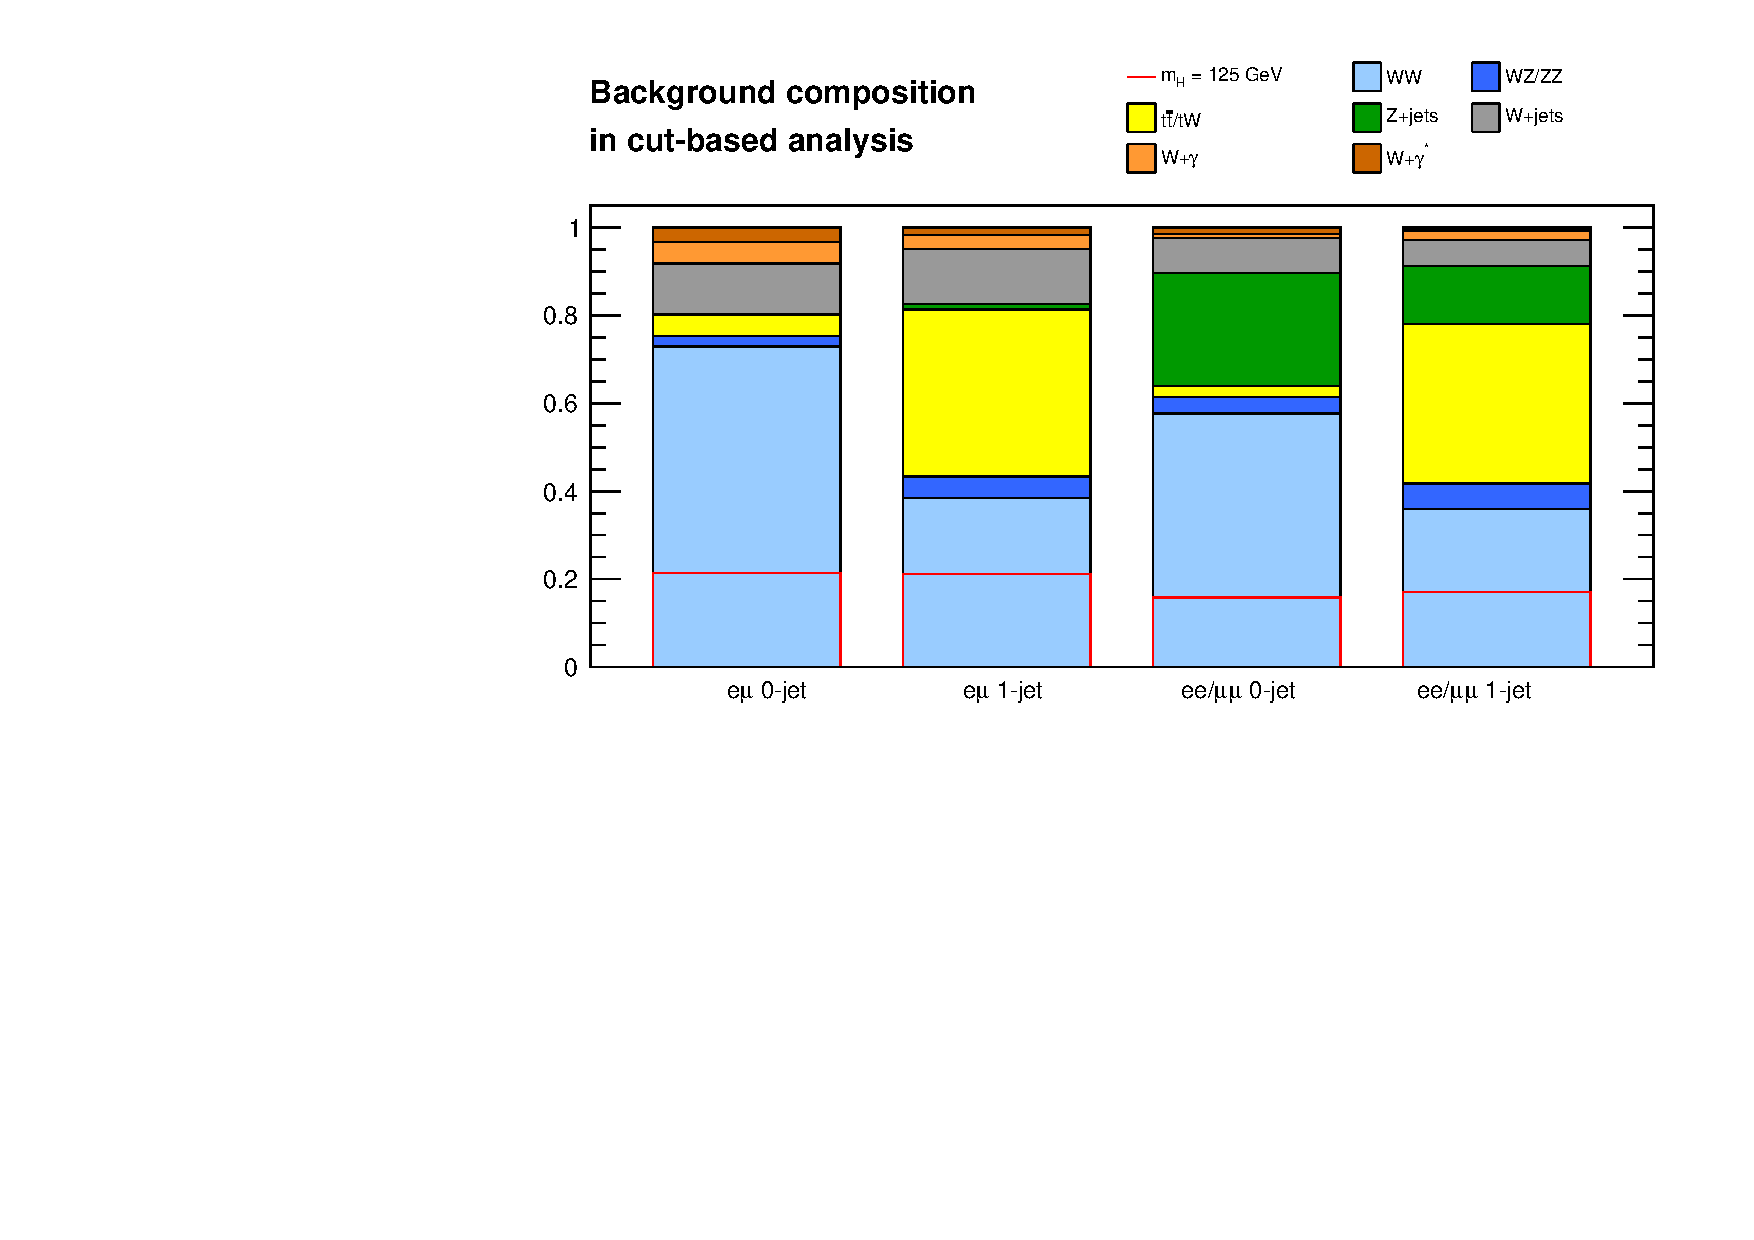
\includegraphics[width=0.99\textwidth]{figures/Bkgcomposition_cutbased.pdf} 
%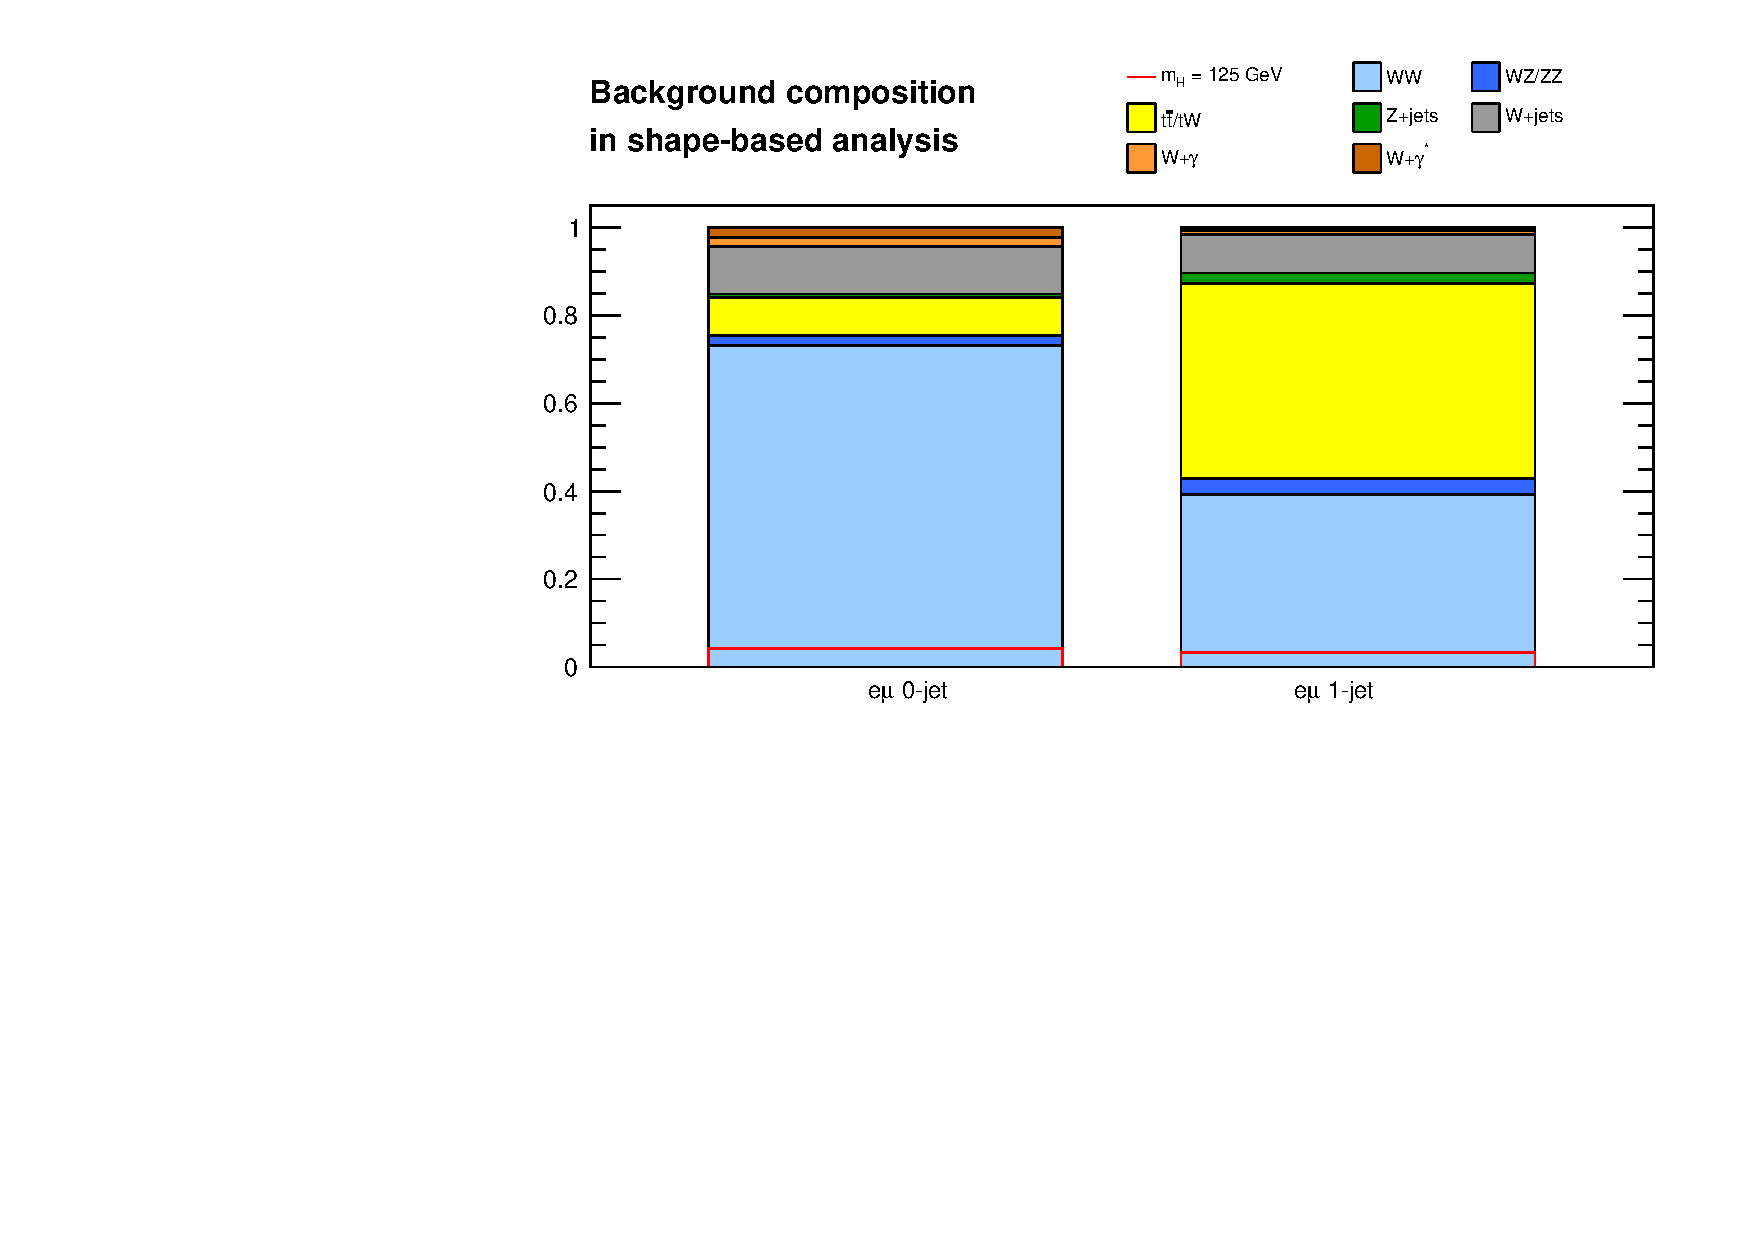
\includegraphics[width=0.9\textwidth]{figures/Bkgcomposition_2d.pdf} 
\end{tabular} 
\caption{Background composition in cut-based analysis for the \mHi=125 \GeV\ hypothesis
in the four categories. 
The Higgs selection in addition to WW selection is applied.  
The signal contribution is overlaid. 
} 
\label{fig:bkgcomposition} 
\end{figure} 

This analysis is dedicated to search for \ggH\ process, 
so the events with 2 or more jets are not considered 
because this region of phase space is used to study the \qqH\ process. 
We thus have two categories in the number of jets(0-jet or 1-jet) 
and two categories in the lepton flavors(\DF\ or \SF). 
Therefore, we have four categories and the dedicated analysis 
is performed in each category. This allows better constraints on the 
backgrounds and thus results in better sensitivity to the discovery.  

The extraction of signal component is done by two methods. 
The first method which is simpler but less sensitive to discovery 
is the ``cut-based" method. This method is a simple cut-and-count approach 
that uses a subset of the selected WW events with enhanced S/B at a given \mHi.
The selections are optimized for a given \mHi,
accounting for the kinematic difference between different \mHi\ hypotheses 
which was discussed in section~\ref{subsec:kinimetic_variables}, 
This method is applied to all lepton flavor final states. 
The other method which is more complicated and sophiscated but more sensitive to discovery 
is the ``shape-based" method which uses binned 2-dimensional templates of \mT\ and \mll. 
A binned maximum likelihood fit to the 2-dimensional templates is performed to extract 
the signal component. The shape-based method uses the difference in shape 
between signal and background, \textit{i.e.}, more information than just normalization, 
so can provide better separation between them. 
In addition, because the fit can constrain backgrounds further than the estimated 
uncertainties, the performance of this method is better than the cut-based method. 
In this method most of the templates are taken from simulation,
so it is important to ensure that the shapes taken from simulation 
are consistent with what is observed in data. 
In the \SF\ channel, the \dyll\ is one of the leading backgrounds, and
the shape of the \dyll\ taken from simulation is not reliable because of the
poor modeling of \met\ and the poor statistics in the sample. So, we apply 
this method to only \DF\ category. 


%%%%%%%%%%%%%%%%%%%%%%%%%%%%%%%%%%%%%%%
\section{Cut-based Method}

%\begin{itemize} 
%\item Motivation of \mHi-dependent cuts : event kinematics different by \mHi 
%\item Physics behind cuts : (1) helicity conservation and V-A nature of W decay (2) more massive Higgs gives harder leptons  
%\item list cut variables: \ptlmax, \ptlmin, \mll, \delphill, \mT 
%\item justify \mHi-dependent cut values : make plots of signal at \mHi=125, 160, 200, 400 GeV
%\item Show the table of \mHi-dependent cuts : make sure that numbers are up-to-date  
%\end{itemize} 

The "cut-based" method is a simple and robust cut-and-count analysis approach. 
In this method, for a given \mHi\ the expected signal and background yields are 
calculated in the region of phase space where S/B is enhanced. 
The yields and the uncertainties of each process are used to determine 
the signal component by a maximum likelihood fit. 
Because the estimated uncertainties are used, the precise estimation
of the uncertainties is very important.  
This method is simpler than the other method because it uses only 
yields(no worries about the shapes), 
and most of the backgrounds are estimated by data-driven methods. 
The issue is the accuracy(normalization) and the precision(uncertainty) of the measurements.  

As described in section~\ref{subsec:kinimetic_variables}, the kinematics of 
the signal events vary depending on \mHi. Therefore, 
in addition to the WW selection, a dedicated selection 
for each \mHi\ point is applied to enhance S/B at the given \mHi. 
We use the following five variables to improve S/B, 
\begin{itemize}
\item lepton transverse momentum : \ptlmax\ and \ptlmin
\item di-lepton mass : \mll 
\item the azimuthal angle difference between the leptons : \delphill
\item Higgs transverse mass : 
\begin{eqnarray} 
\mT = \sqrt{2\ptll\met(1-cos(\Delta\phi_{\ell\ell-\met}))}
\end{eqnarray} 
where \ptll\ is the transverse momentum of the di-lepton system,
\met\ is the missing transverse momentum and
$\Delta\phi_{\ell\ell-\met}$ is the angle between di-lepton
direction and \met\ in the transverse plane.
\end{itemize}

% WW-level mH = 125 GeV
\begin{figure}[htp]
\centering
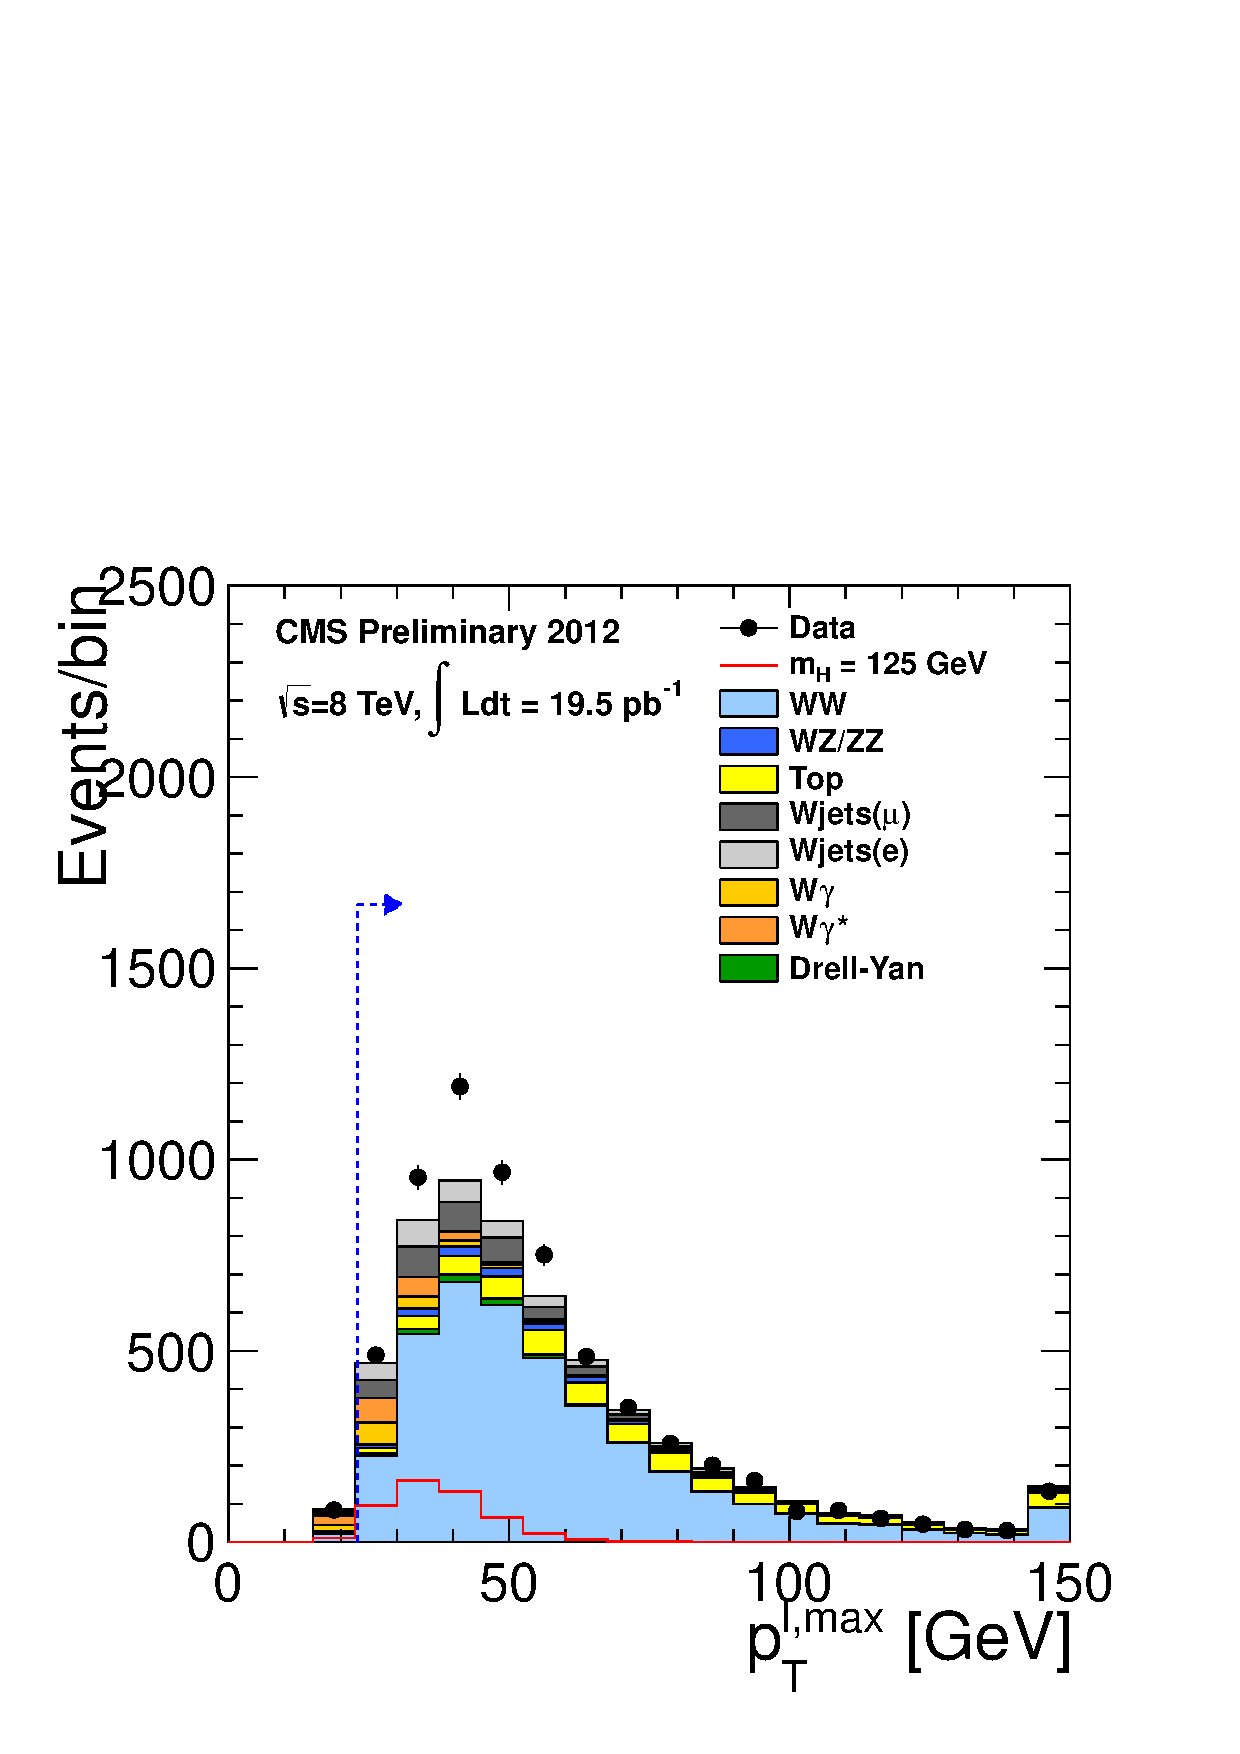
\includegraphics[width=0.45\textwidth]{figures/hww_analysis16_125_ALL_of_0j_pt1.pdf}
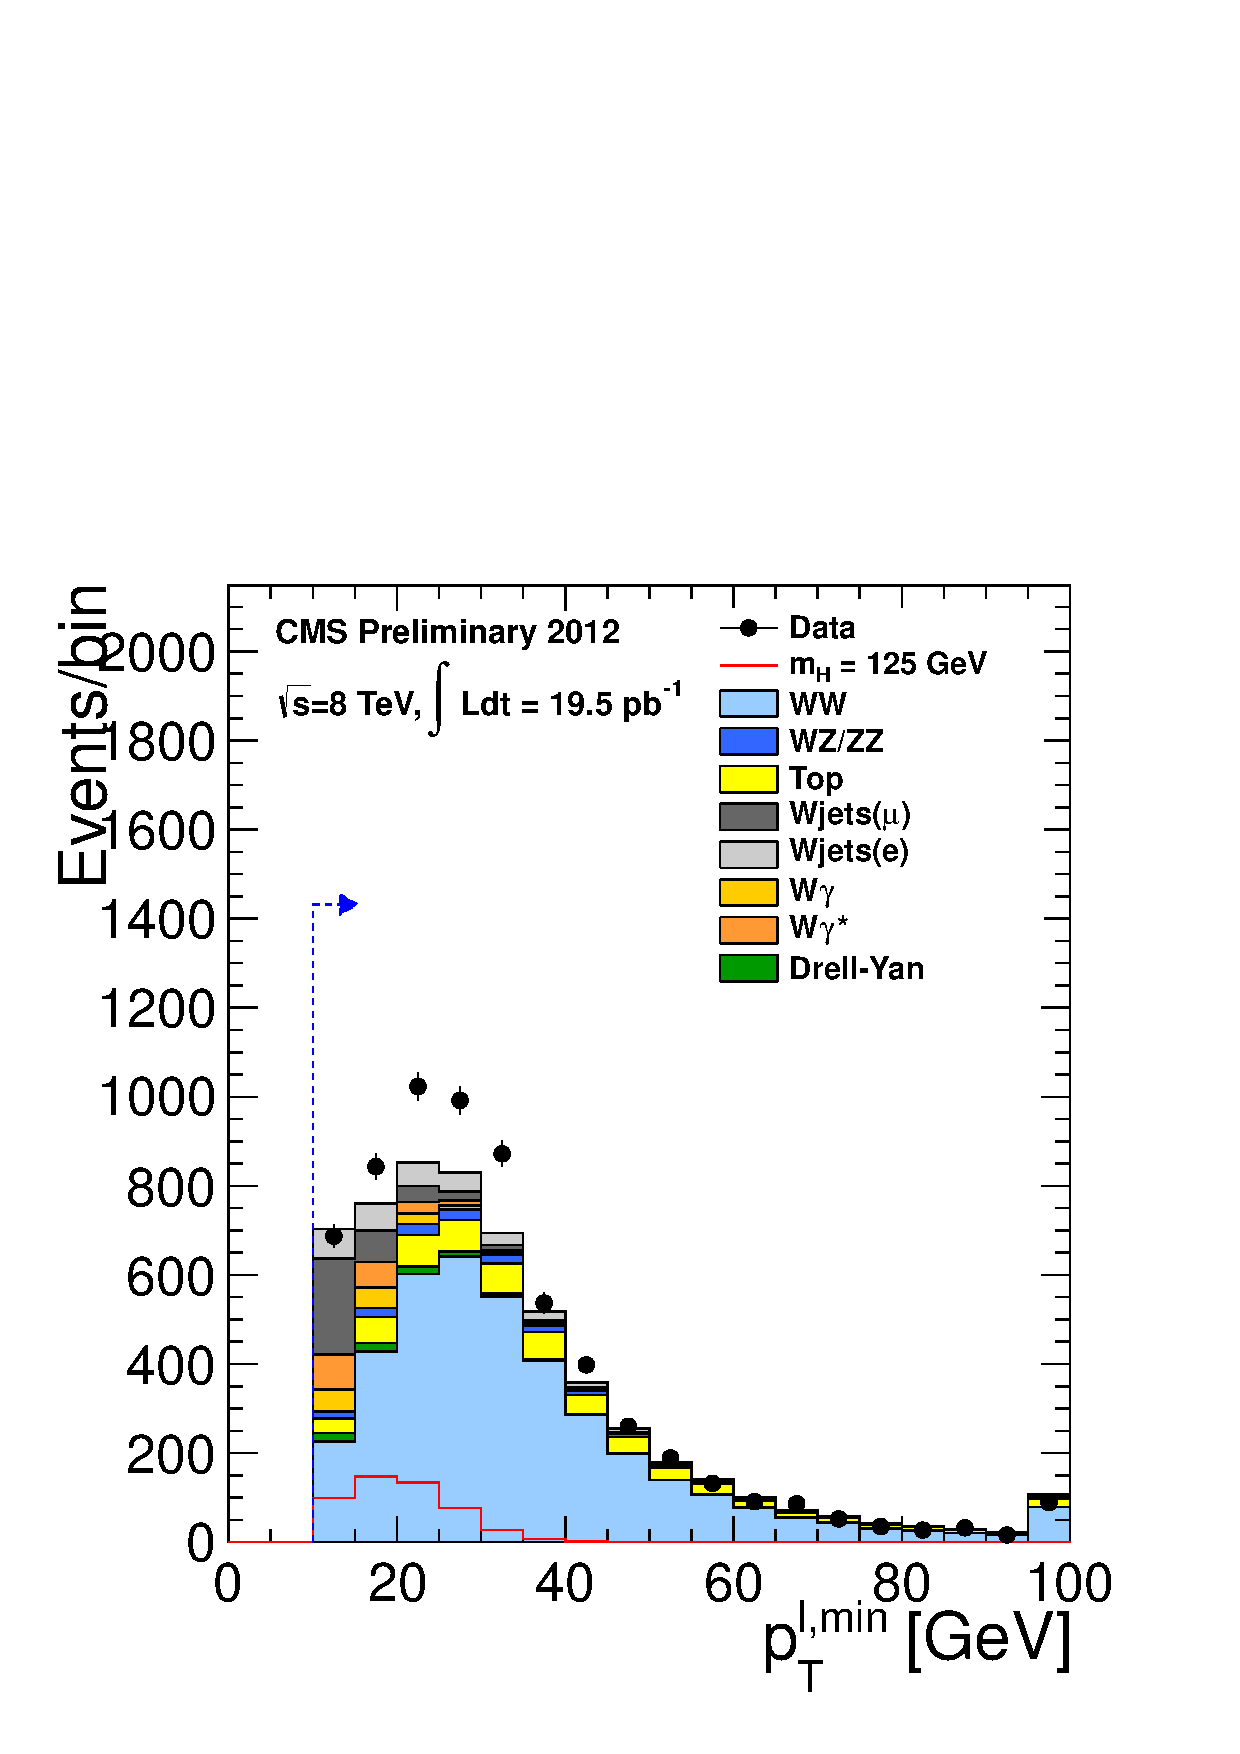
\includegraphics[width=0.45\textwidth]{figures/hww_analysis16_125_ALL_of_0j_pt2.pdf}
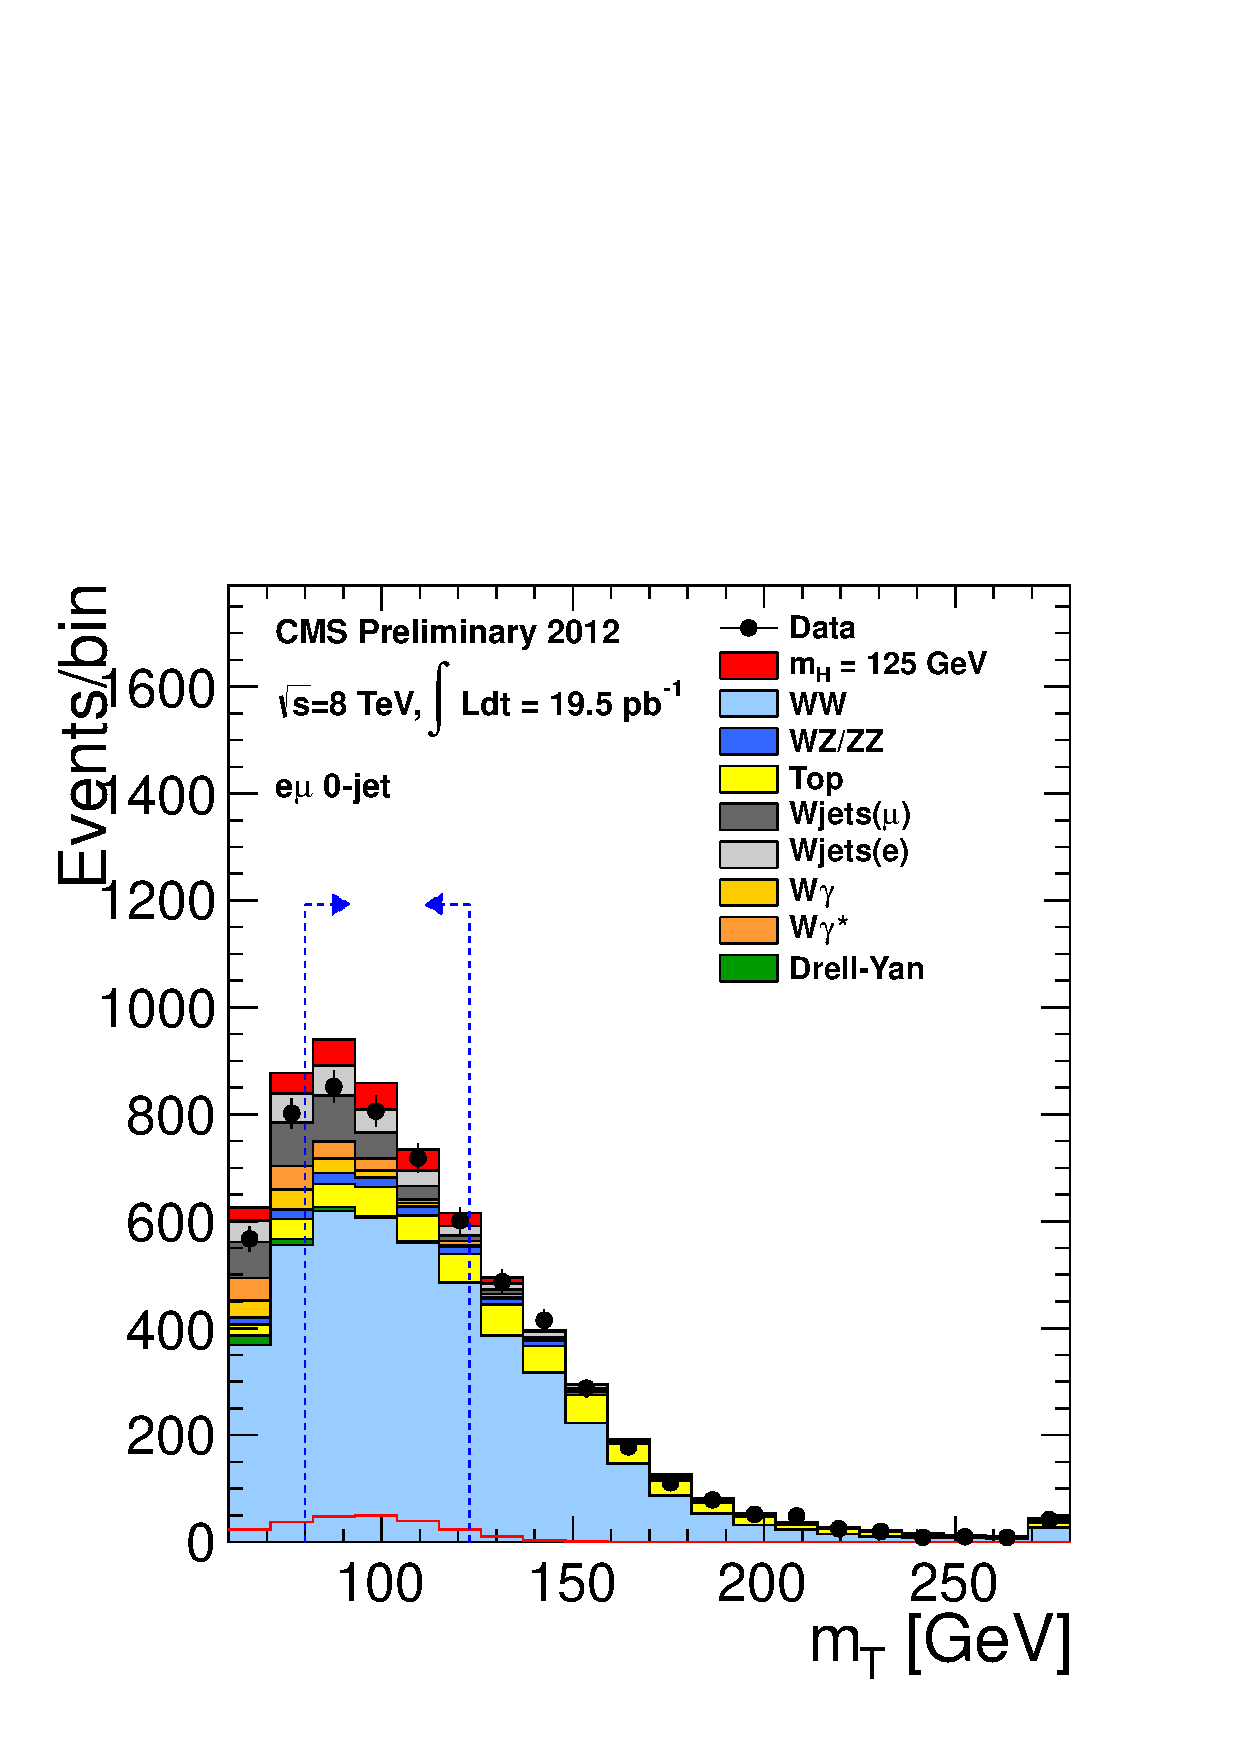
\includegraphics[width=0.45\textwidth]{figures/hww_analysis16_125_ALL_of_0j_mt.pdf}
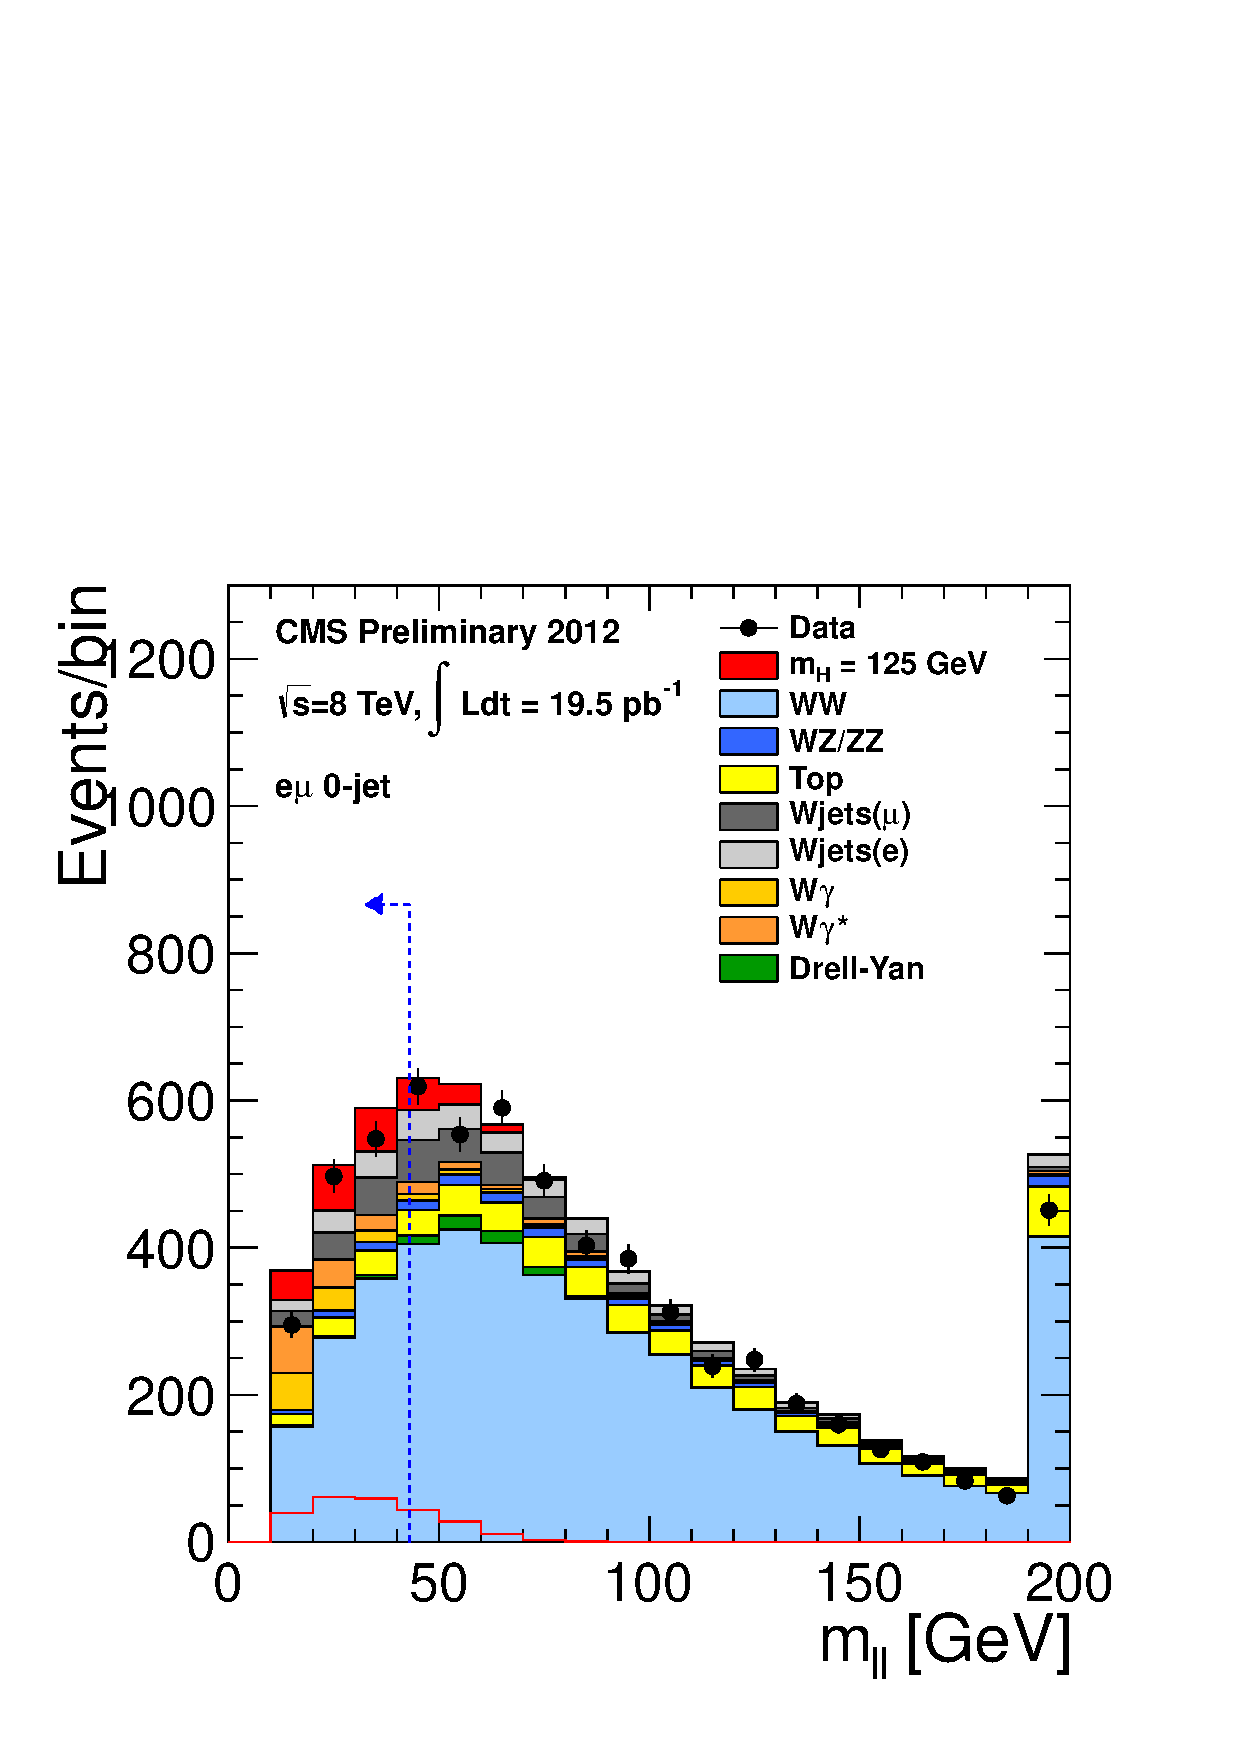
\includegraphics[width=0.45\textwidth]{figures/hww_analysis16_125_ALL_of_0j_mll.pdf}
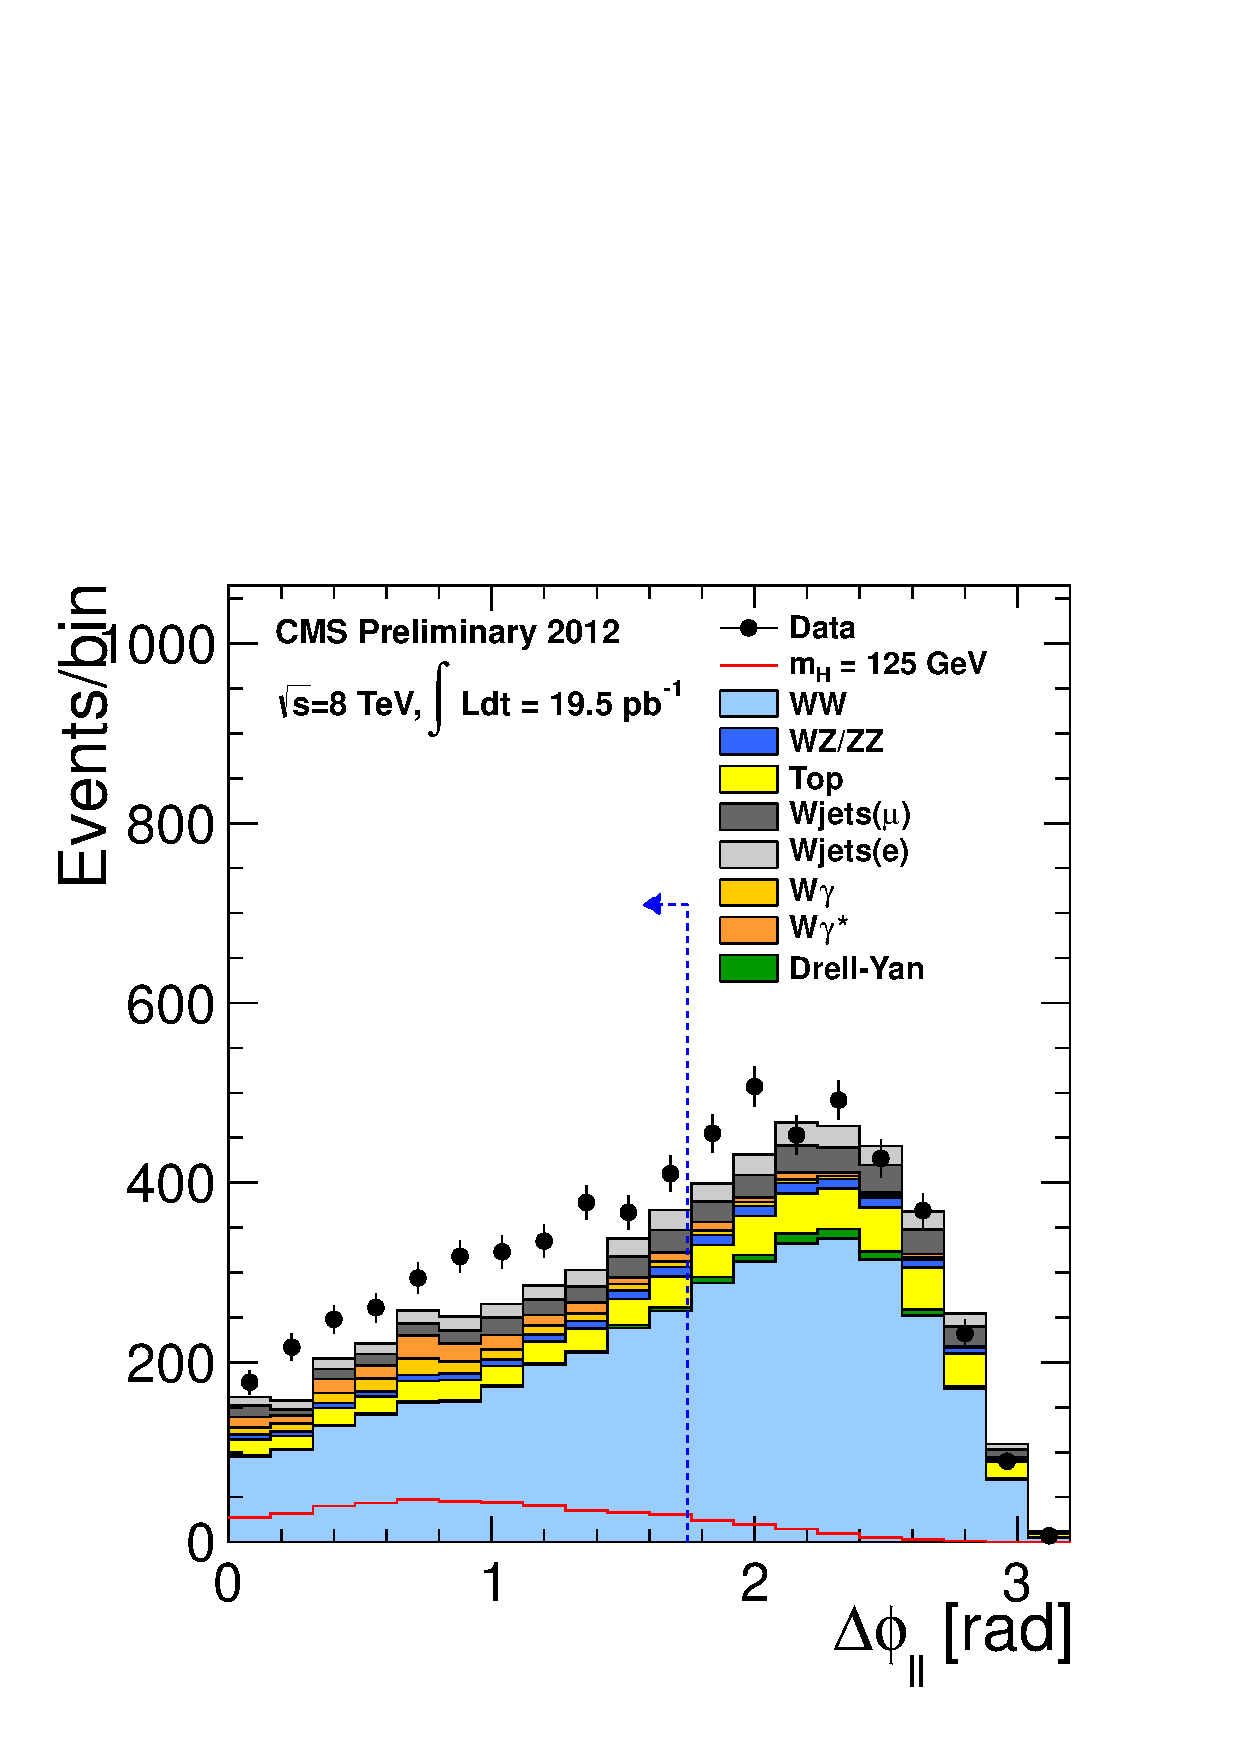
\includegraphics[width=0.45\textwidth]{figures/hww_analysis16_125_ALL_of_0j_dphi.pdf}
%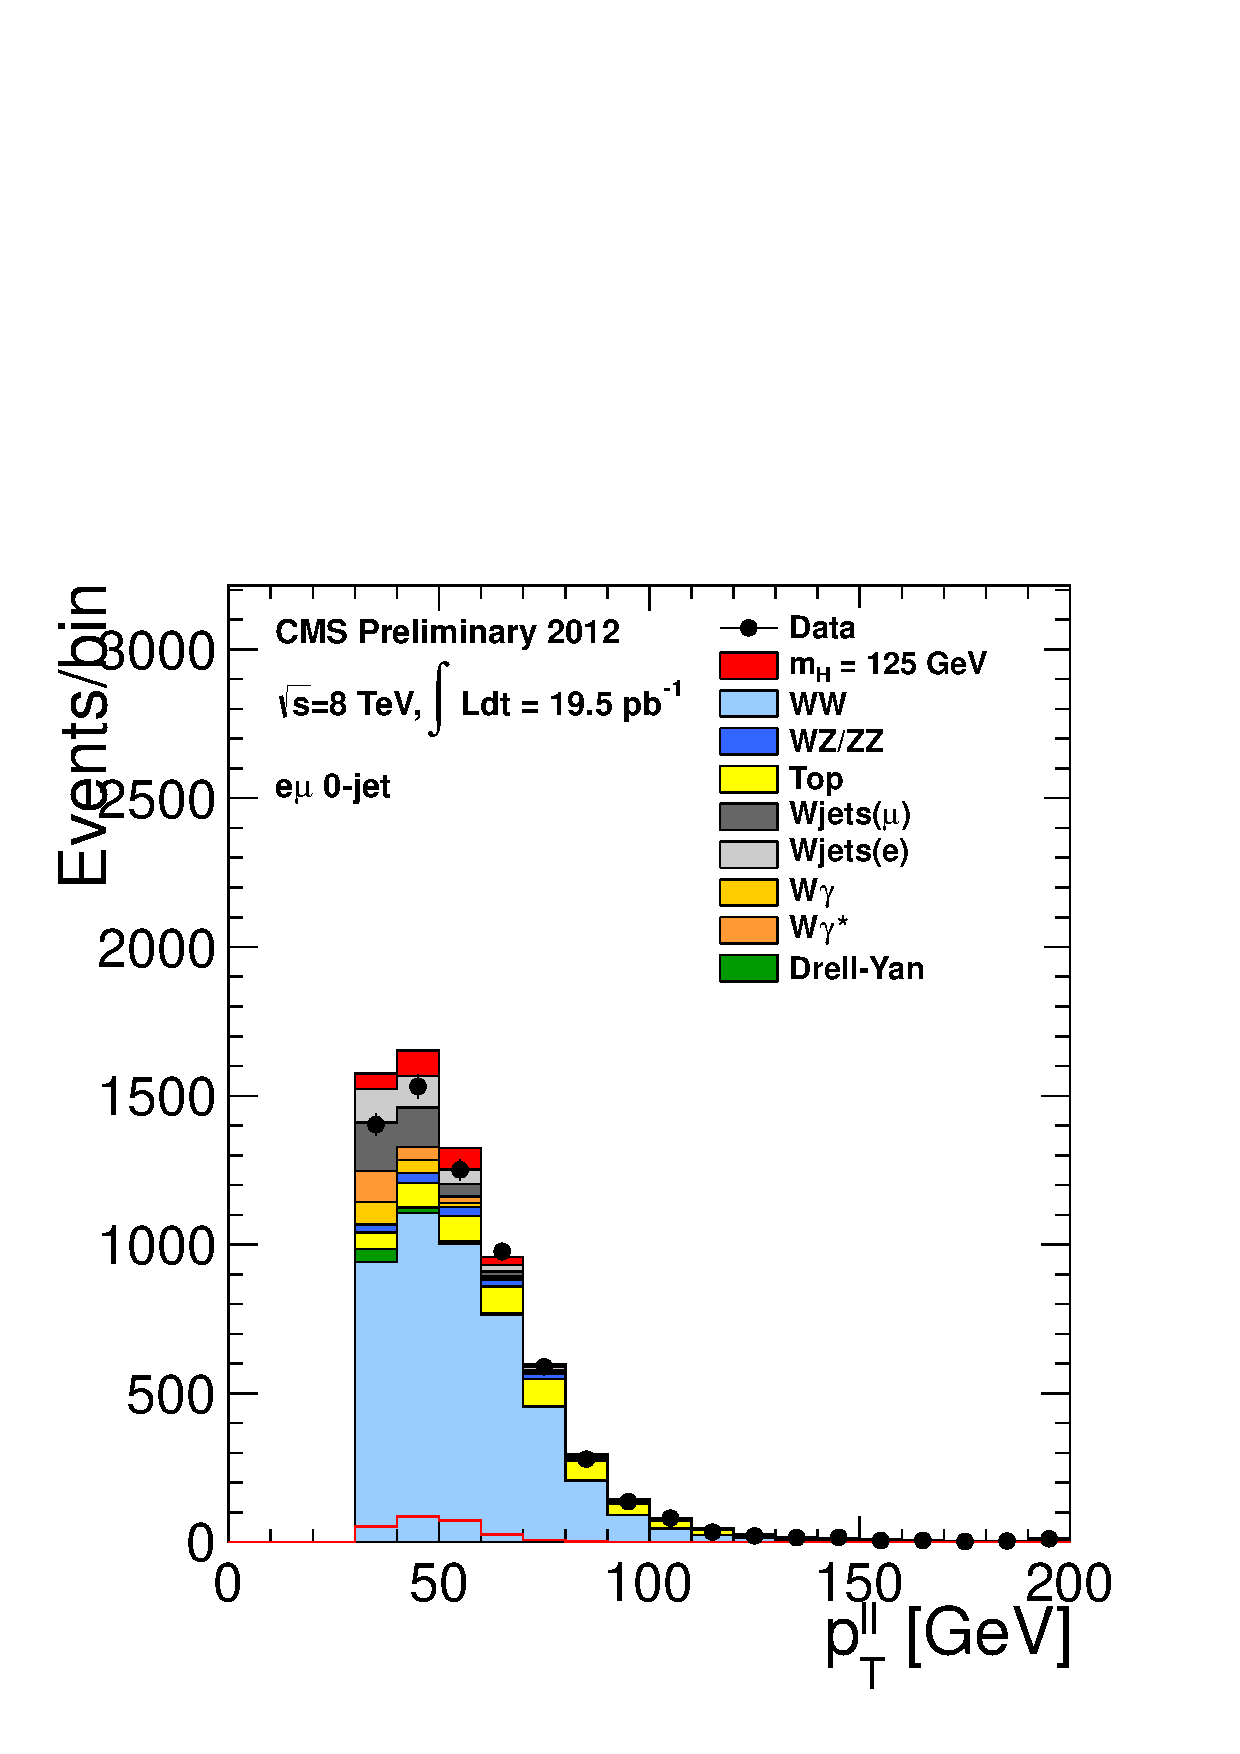
\includegraphics[width=0.45\textwidth]{figures/hww_analysis16_125_ALL_of_0j_ptll.pdf}
\caption{ WW-level plots in 0-jet \DF\ channel with \mHi=125~\GeV\ signal overlaid. 
Cuts for \mHi=125~\GeV\ is shown with blue dotted lines and arrows. 
}
\label{fig:wwlevelmh125}
\end{figure}

% WW-level mH = 160 GeV
\begin{figure}[htp]
\centering
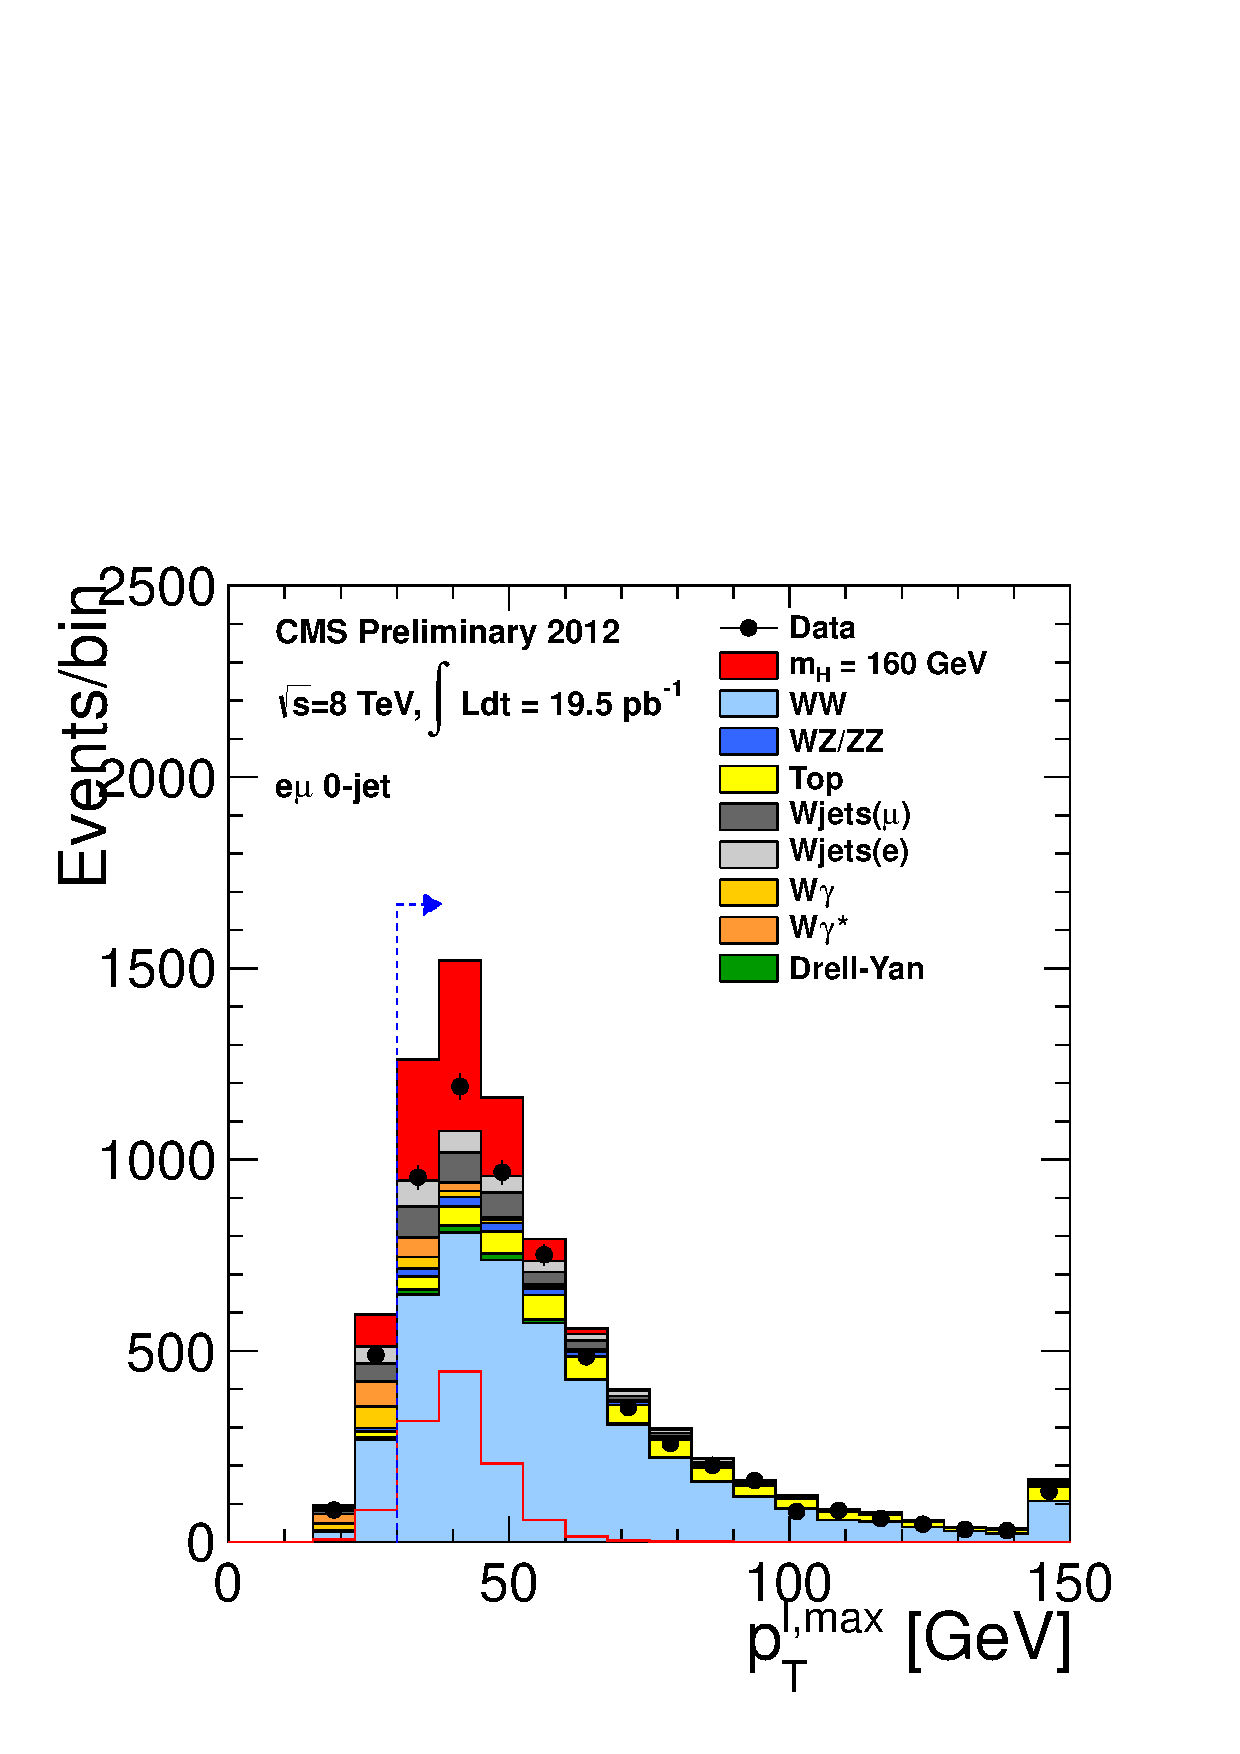
\includegraphics[width=0.45\textwidth]{figures/hww_analysis16_160_ALL_of_0j_pt1.pdf}
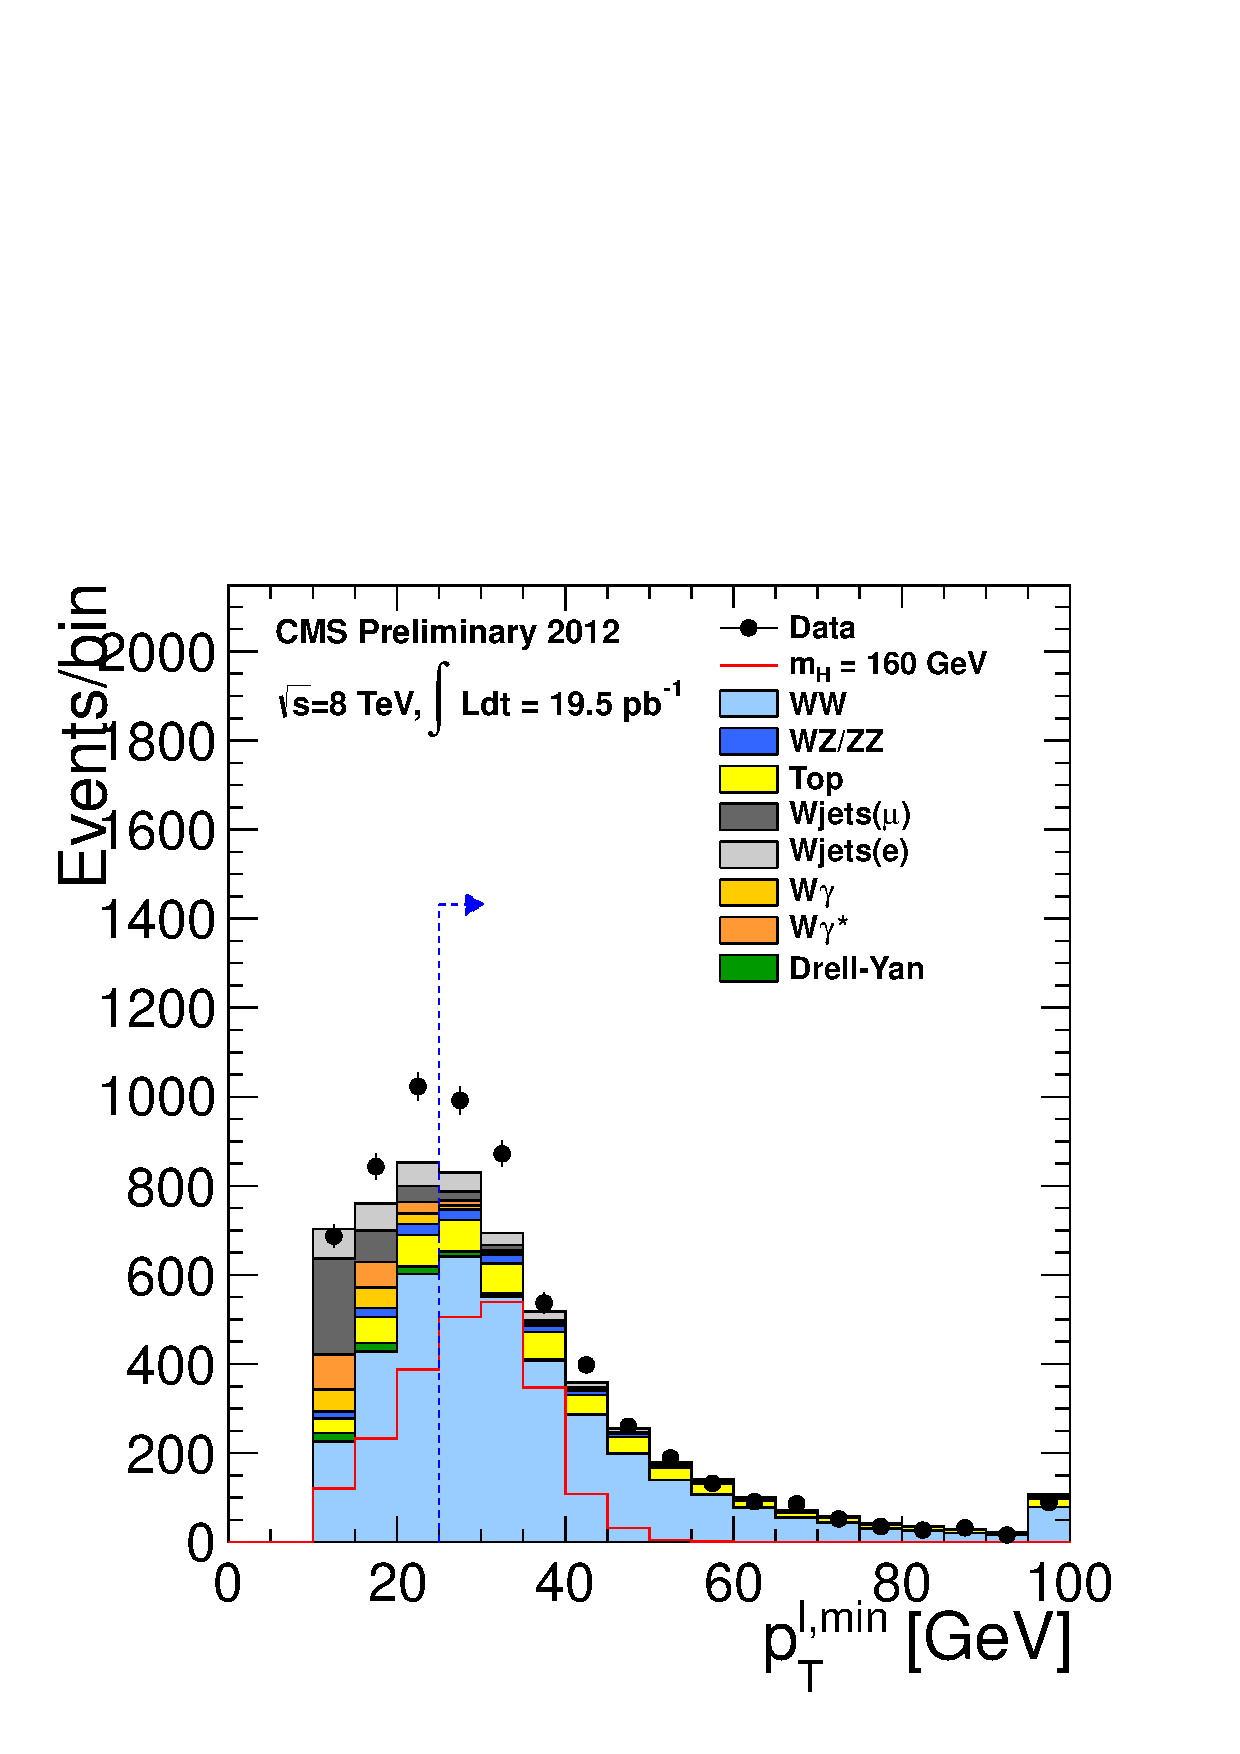
\includegraphics[width=0.45\textwidth]{figures/hww_analysis16_160_ALL_of_0j_pt2.pdf}
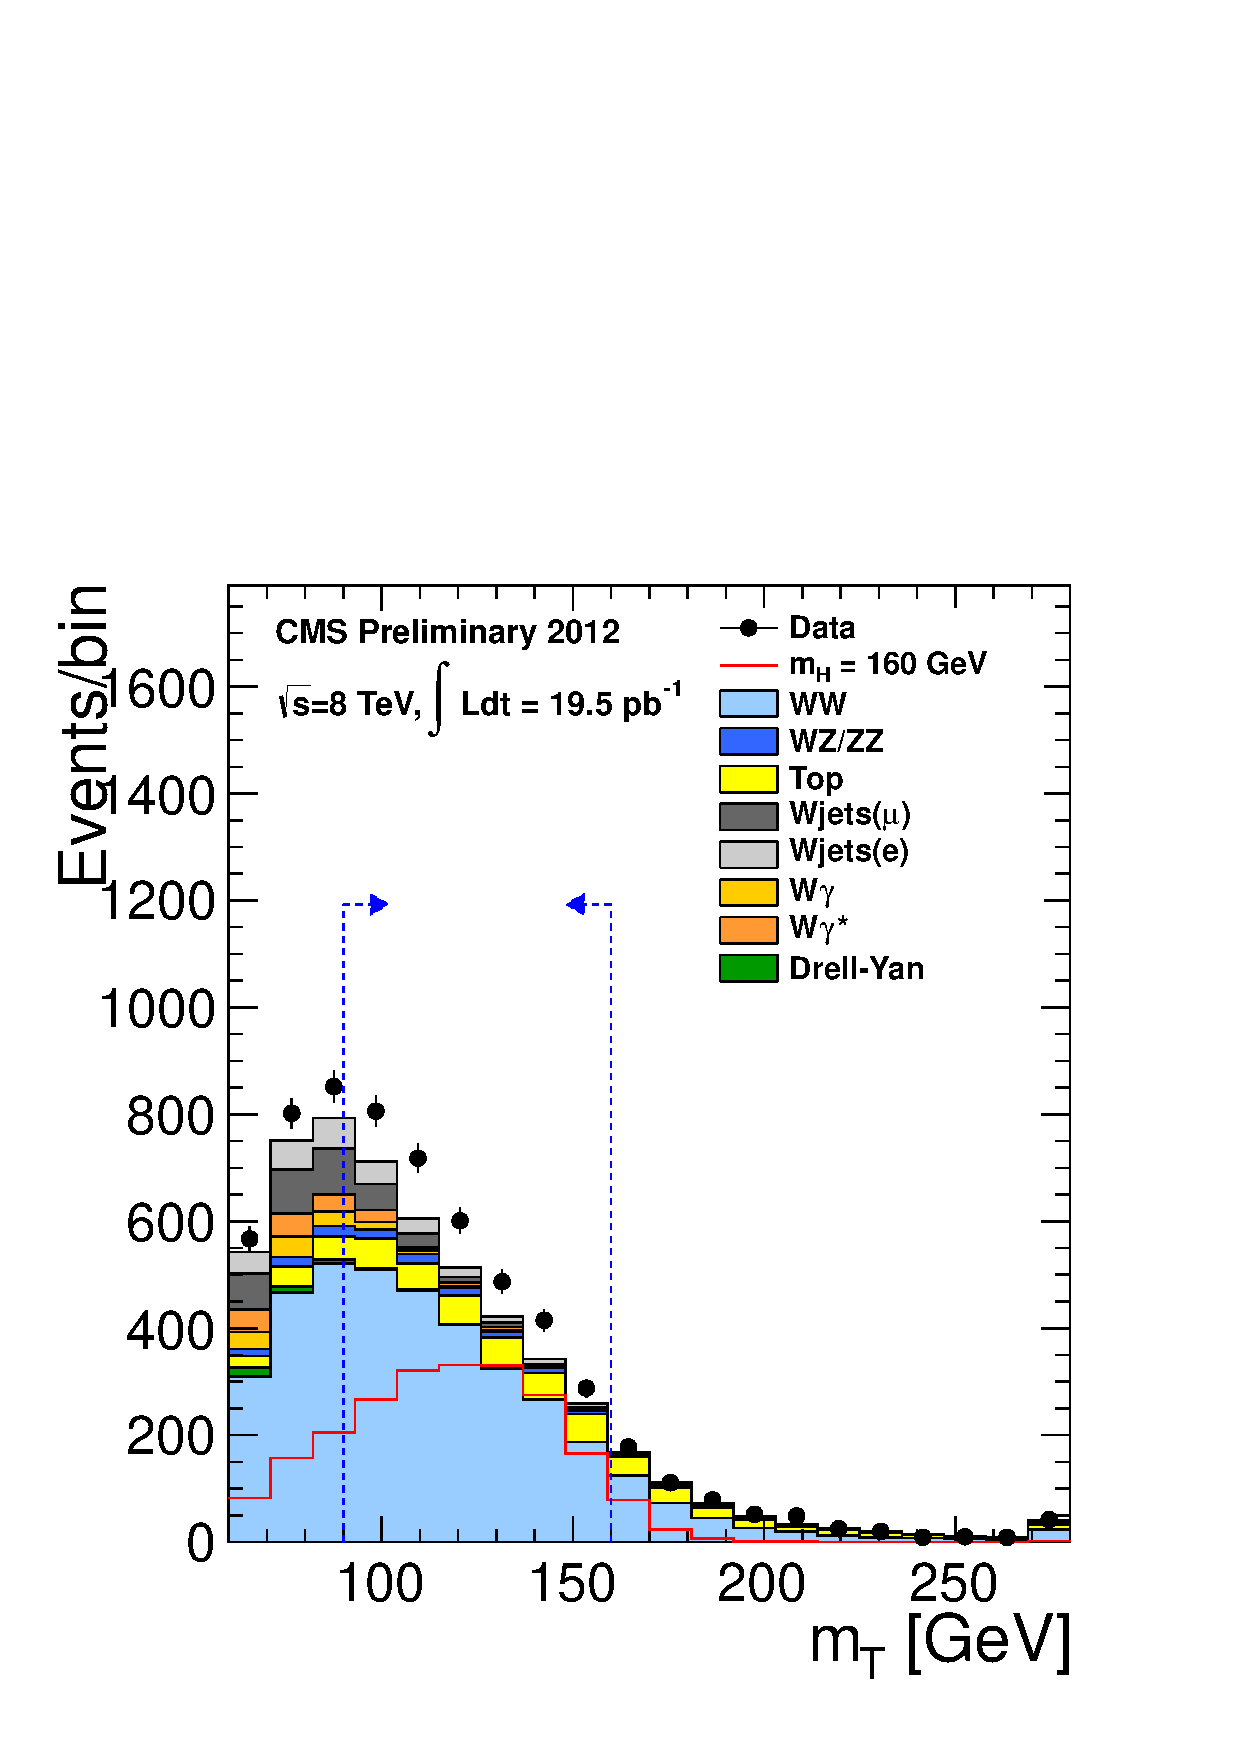
\includegraphics[width=0.45\textwidth]{figures/hww_analysis16_160_ALL_of_0j_mt.pdf}
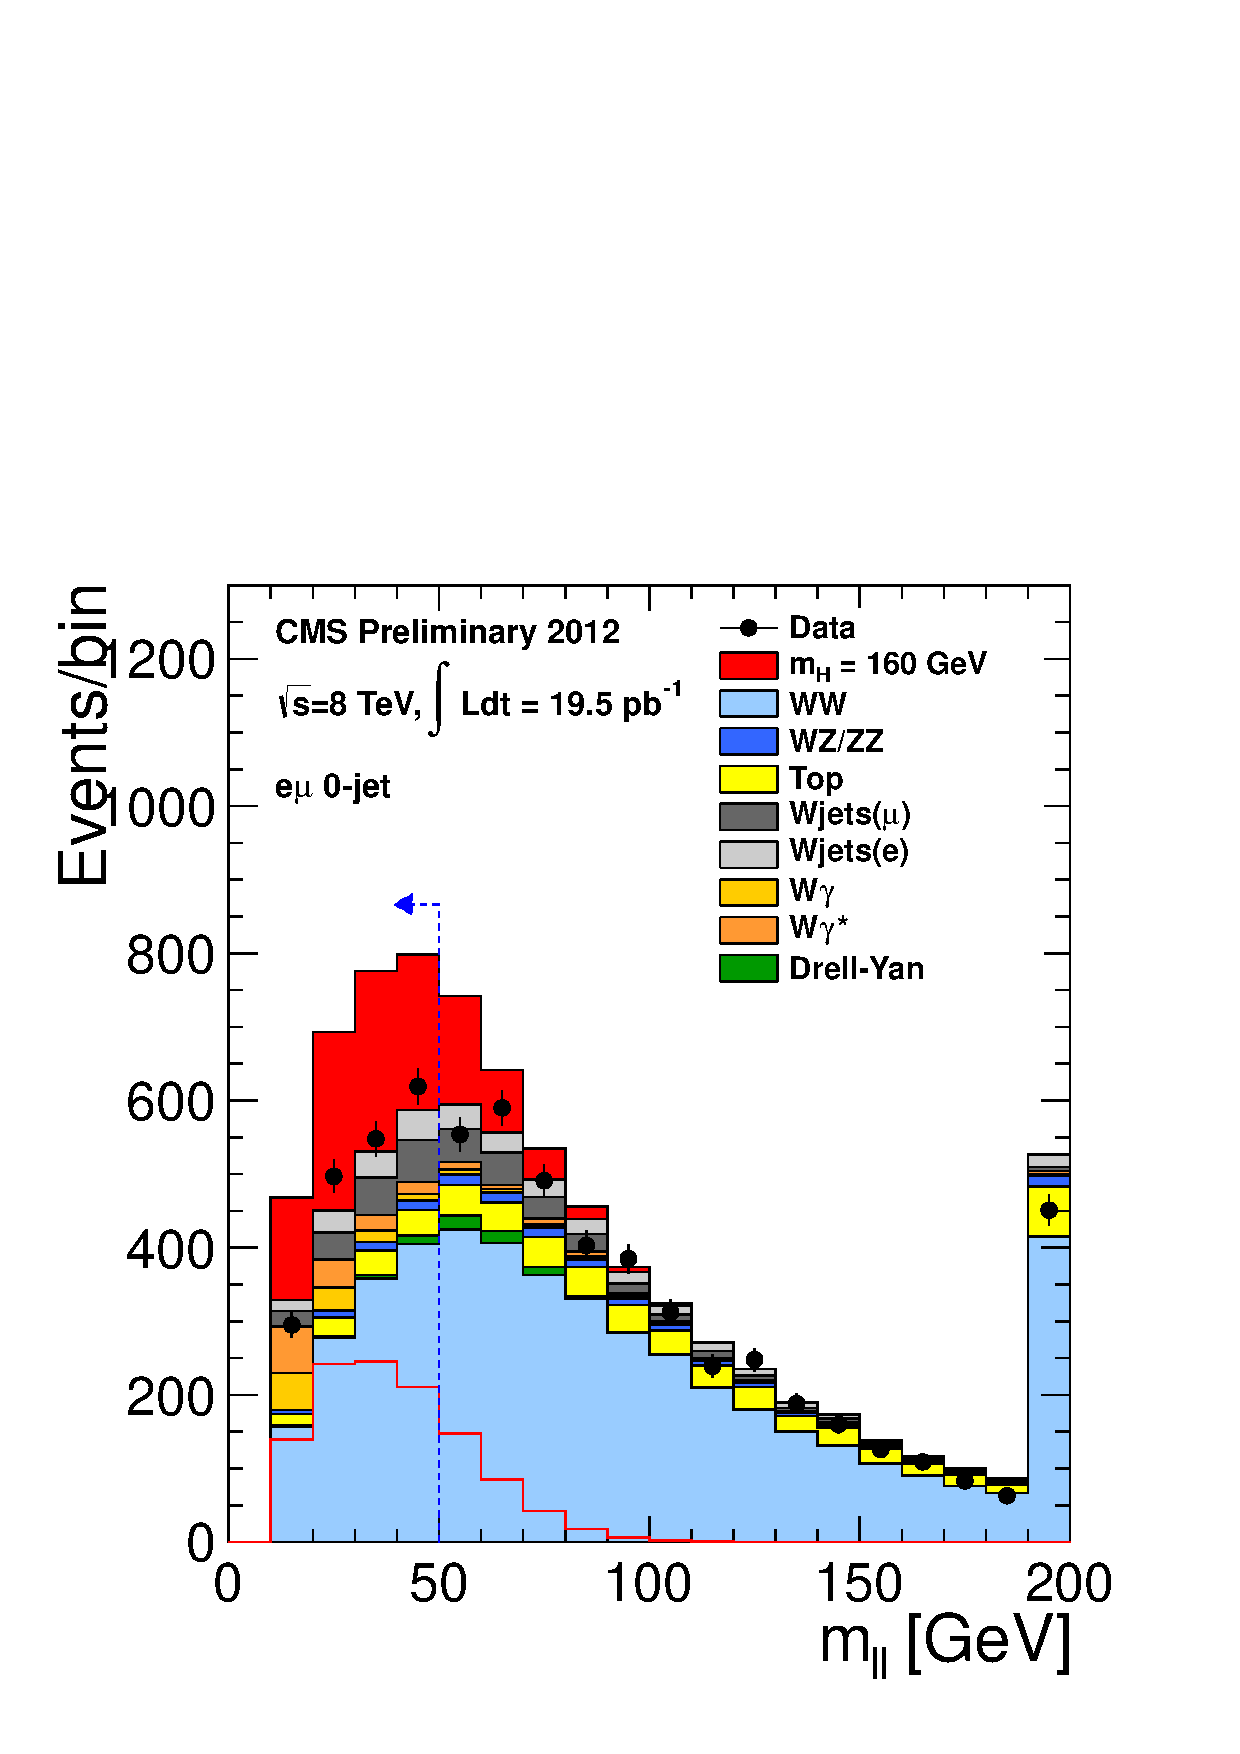
\includegraphics[width=0.45\textwidth]{figures/hww_analysis16_160_ALL_of_0j_mll.pdf}
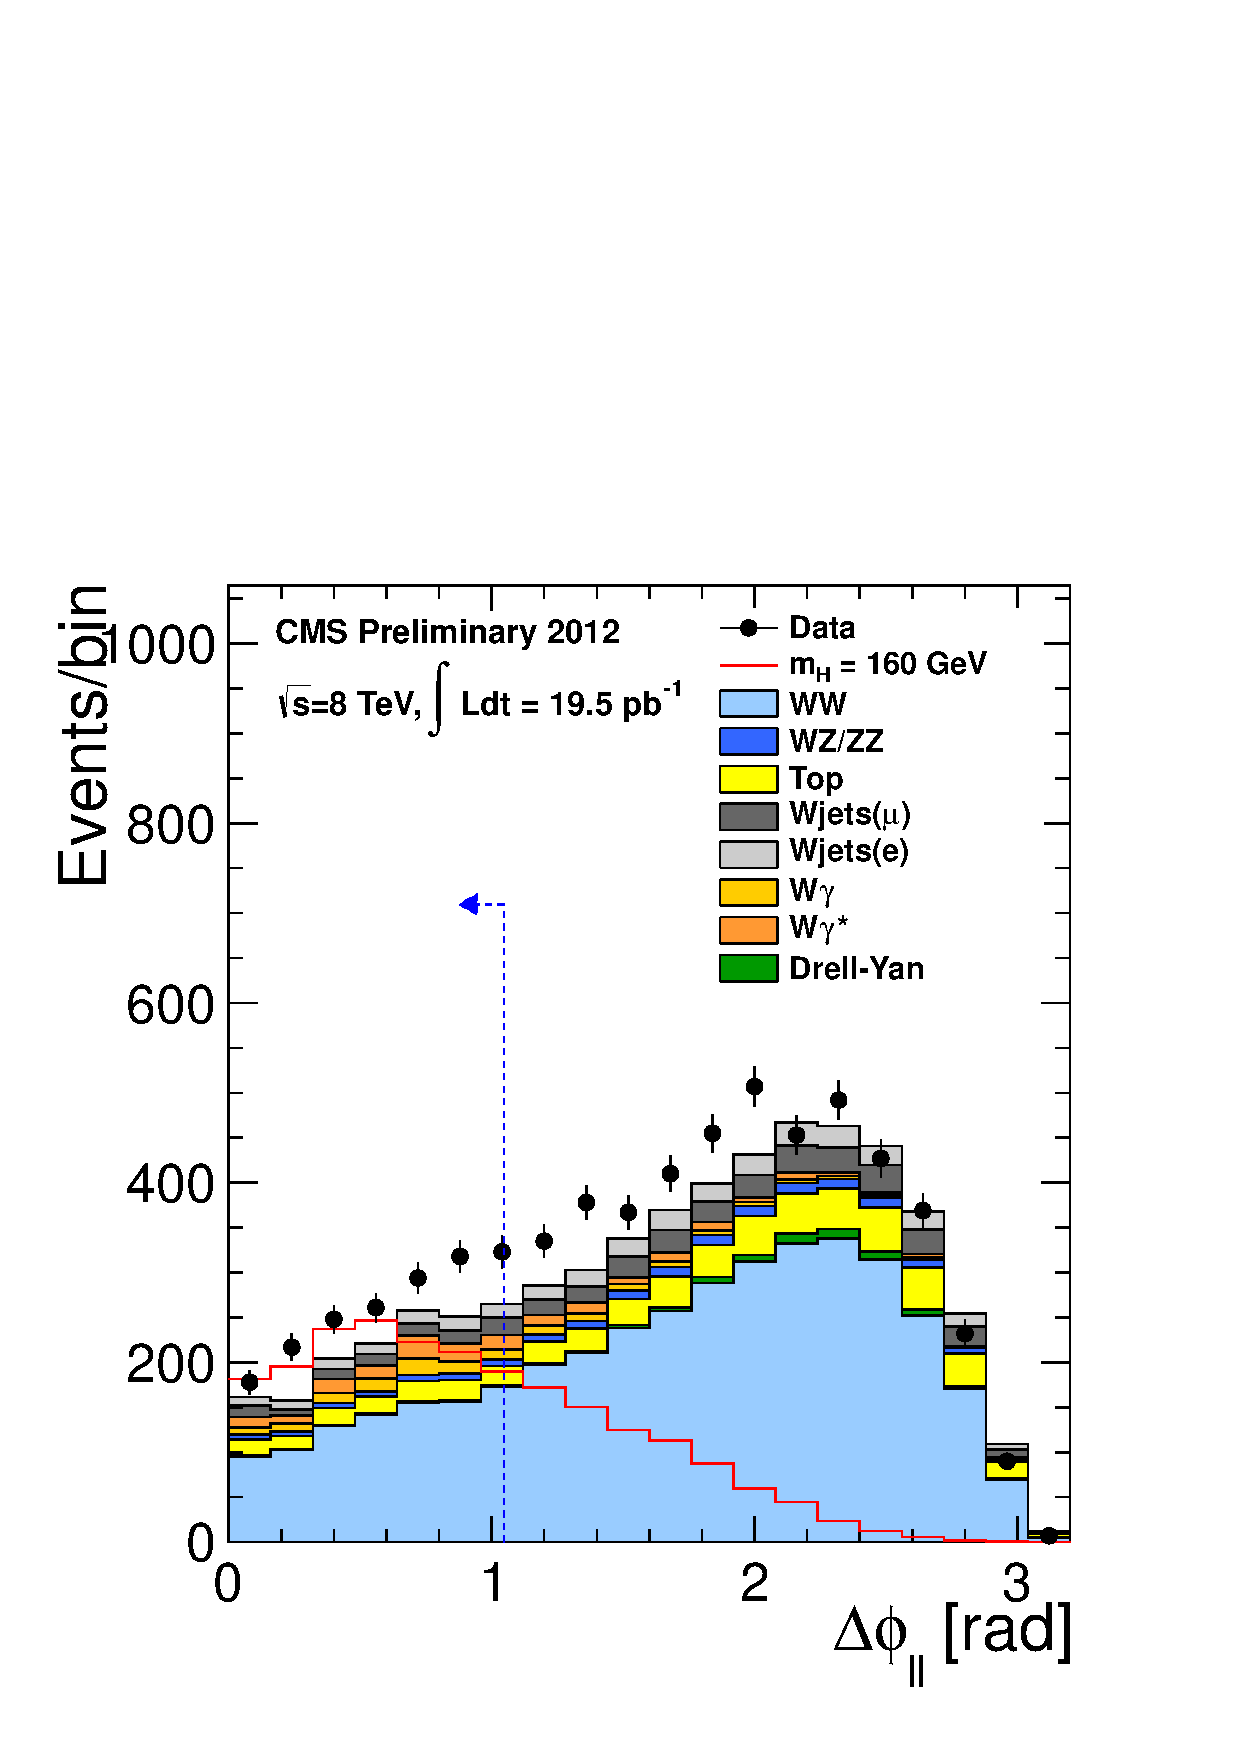
\includegraphics[width=0.45\textwidth]{figures/hww_analysis16_160_ALL_of_0j_dphi.pdf}
%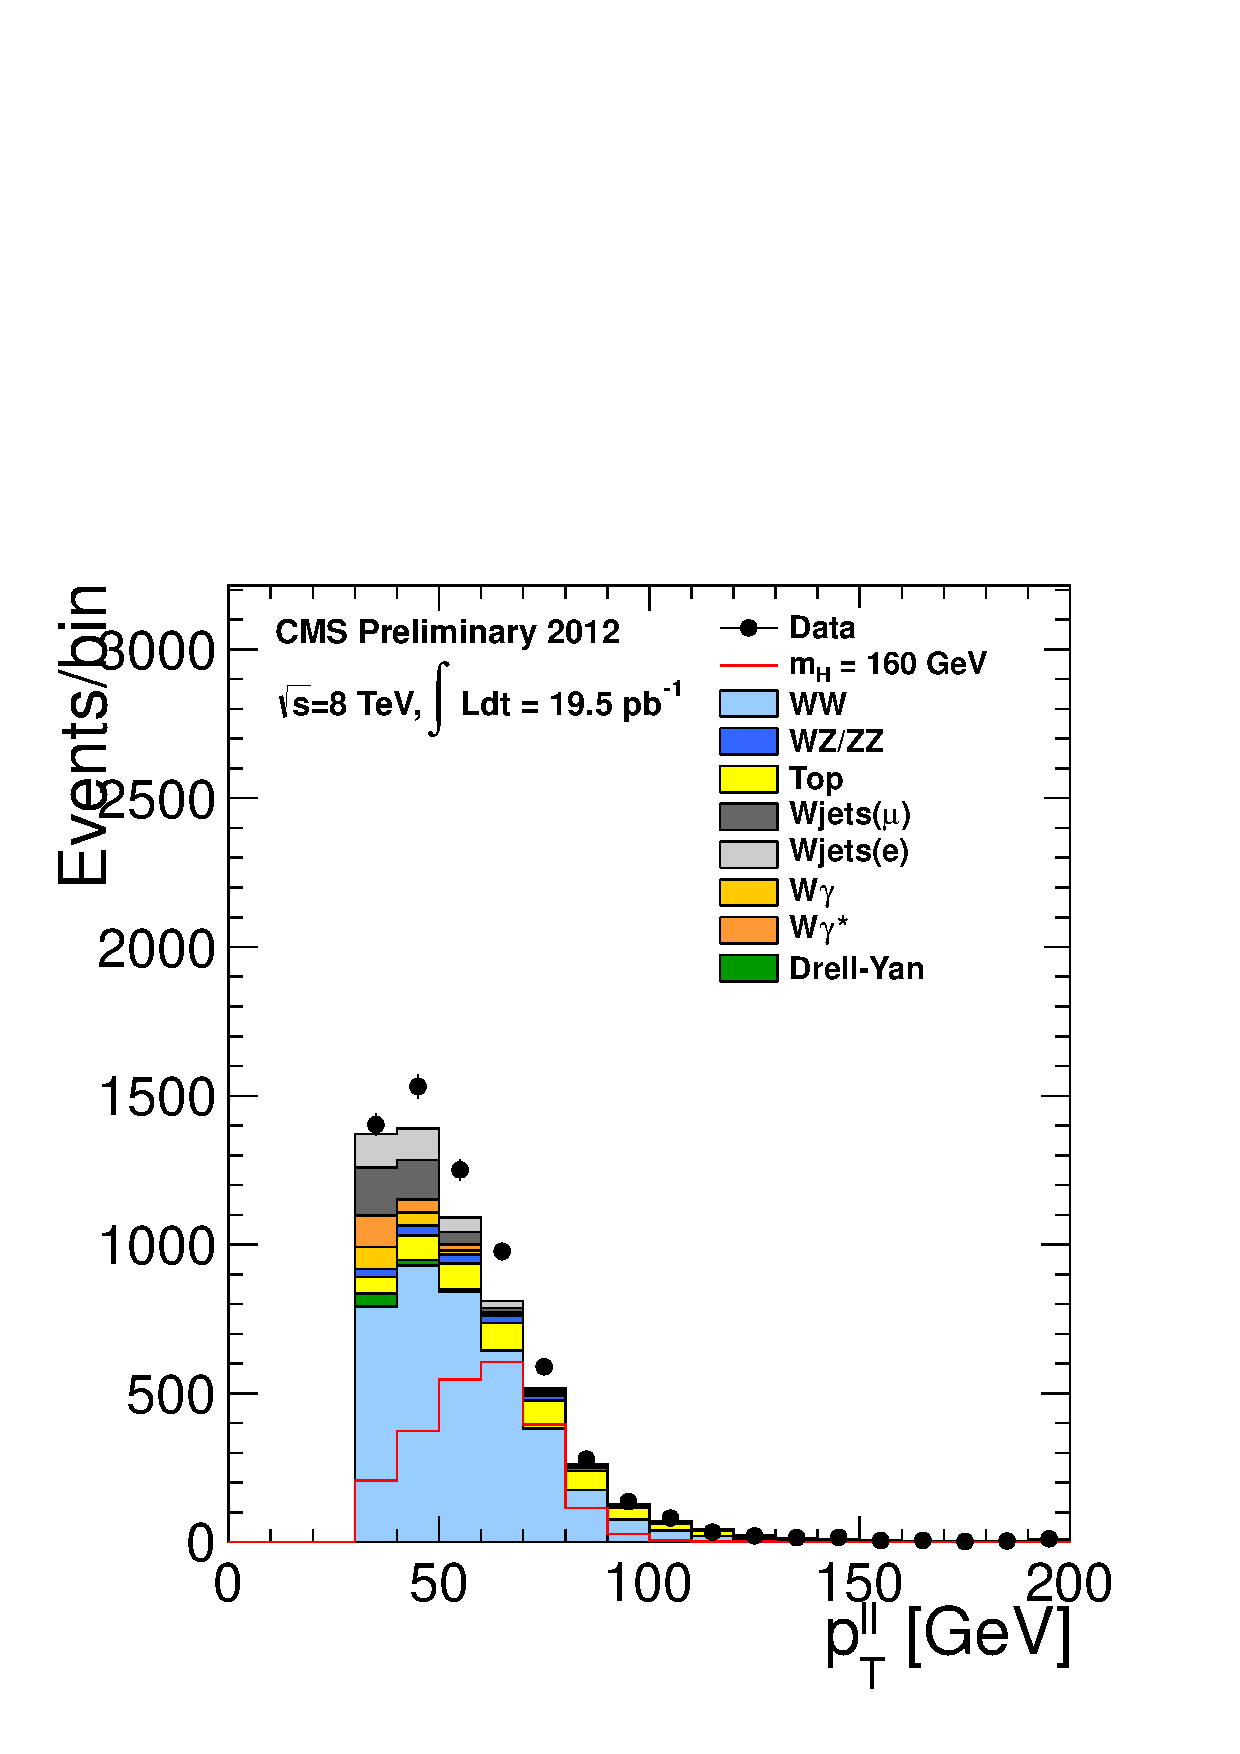
\includegraphics[width=0.45\textwidth]{figures/hww_analysis16_160_ALL_of_0j_ptll.pdf}
\caption{ WW-level plots in 0-jet \DF\ channel with \mHi=160~\GeV\ signal overlaid. 
Cuts for \mHi=160~\GeV\ is shown with blue dotted lines and arrows. 
}
\label{fig:wwlevelmh160}
\end{figure}

% WW-level mH = 200 GeV
\begin{figure}[htp]
\centering
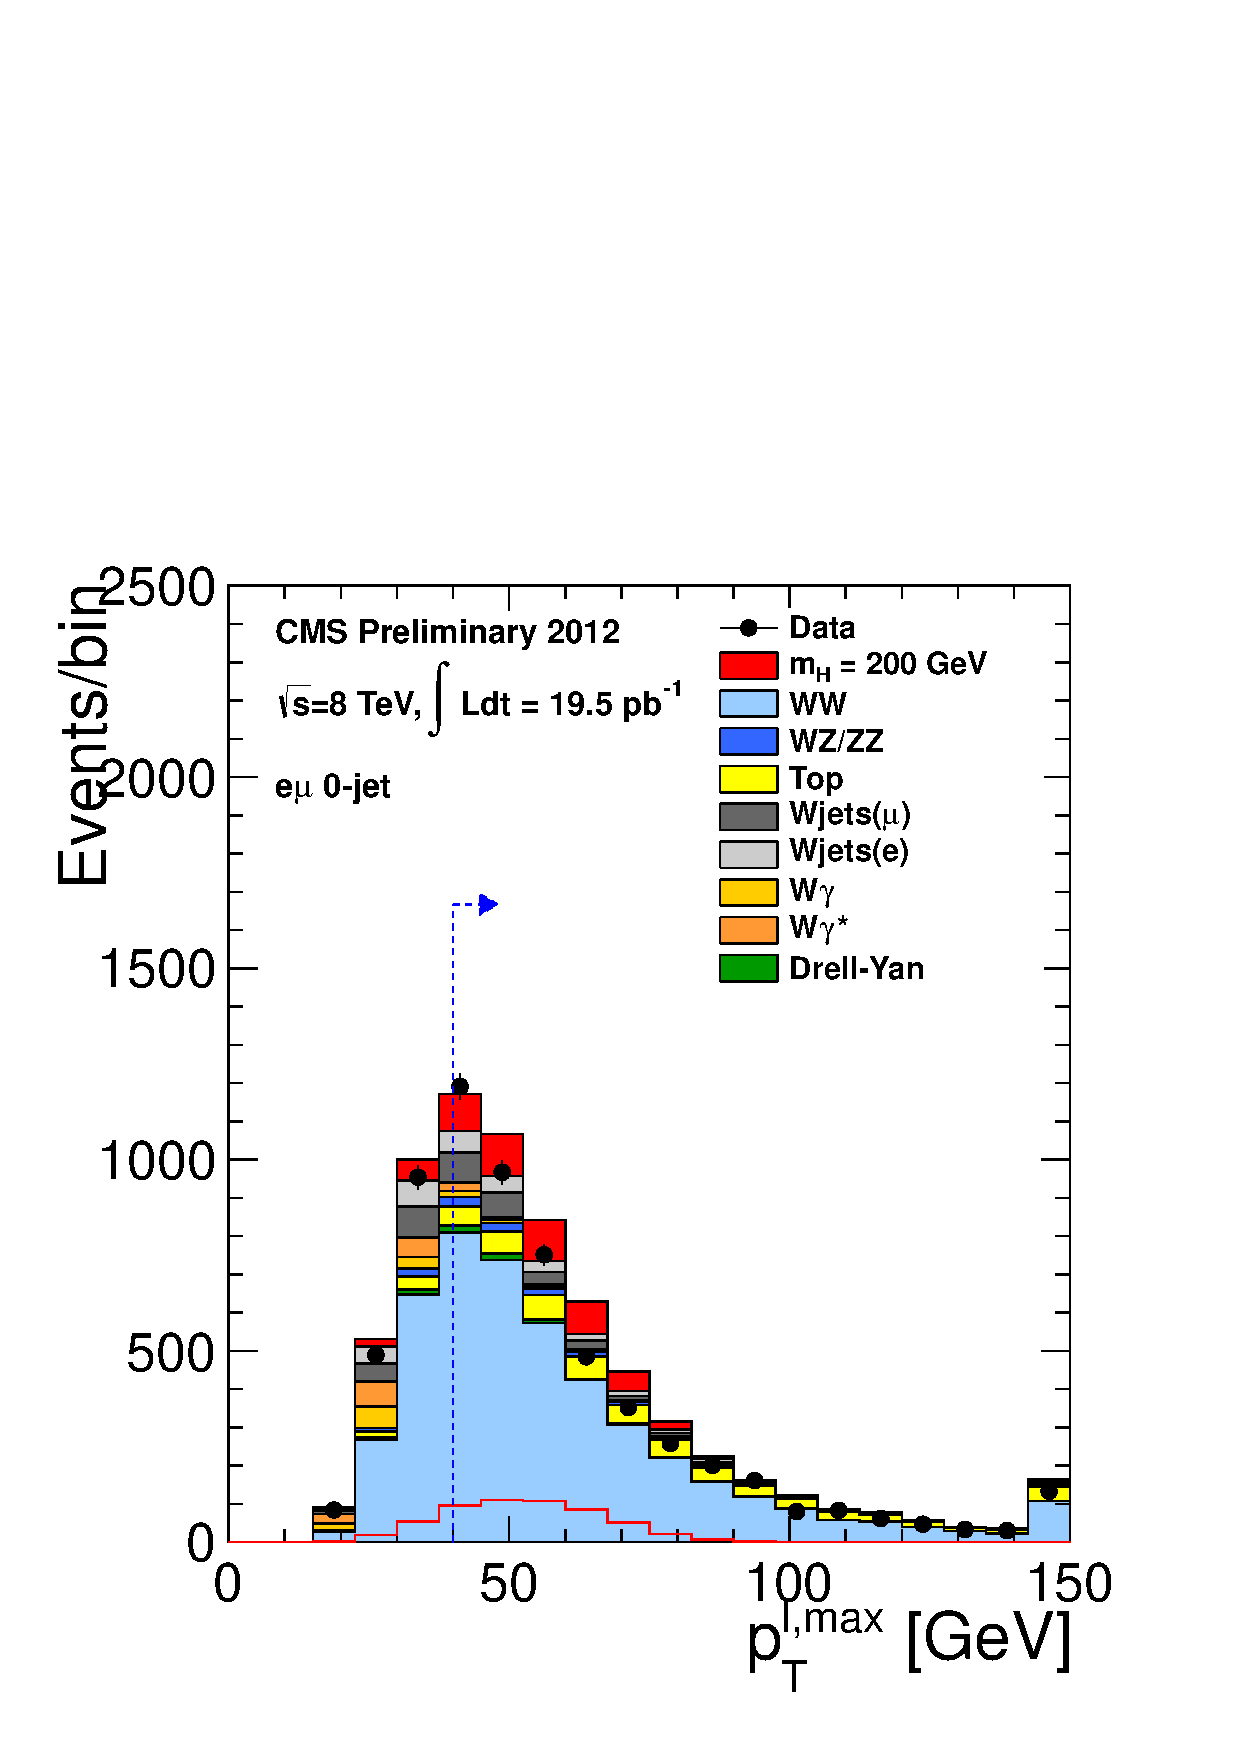
\includegraphics[width=0.45\textwidth]{figures/hww_analysis16_200_ALL_of_0j_pt1.pdf}
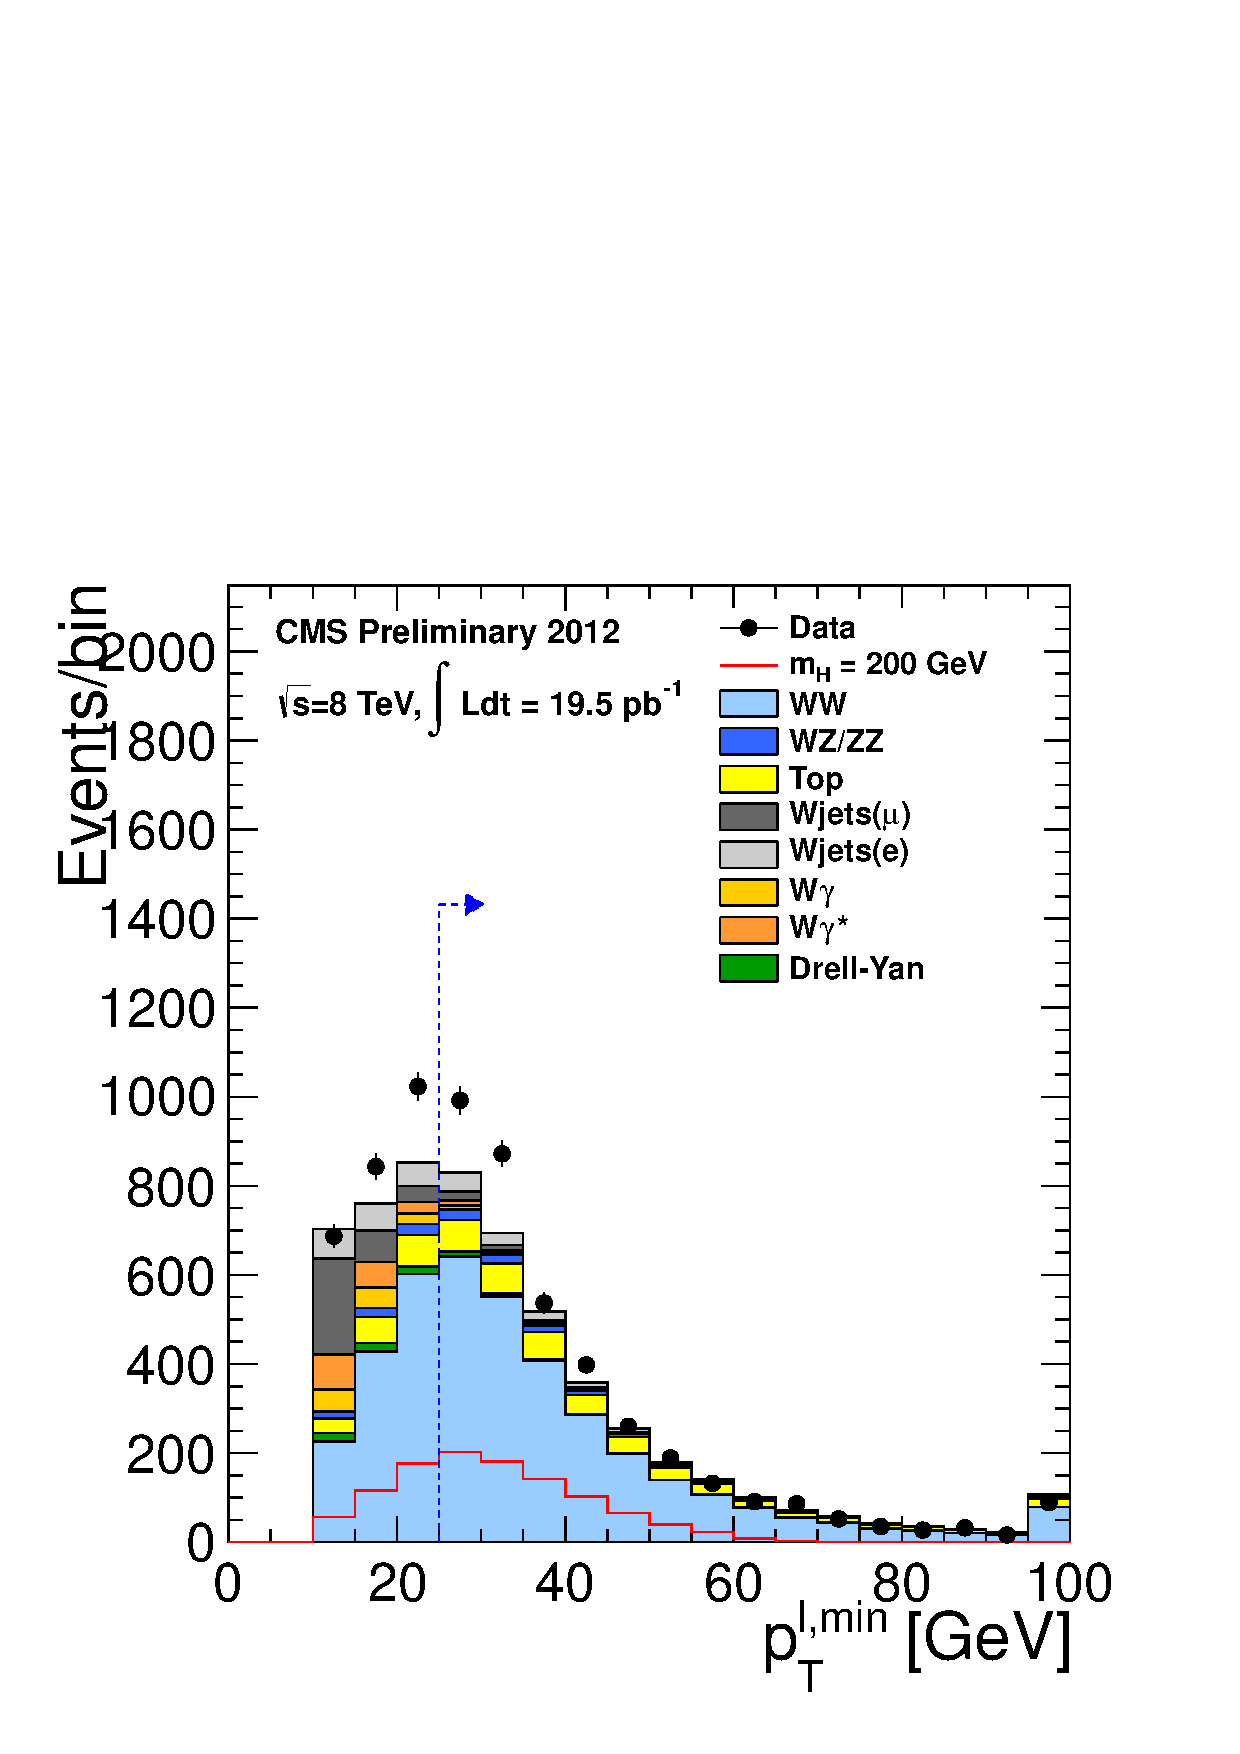
\includegraphics[width=0.45\textwidth]{figures/hww_analysis16_200_ALL_of_0j_pt2.pdf}
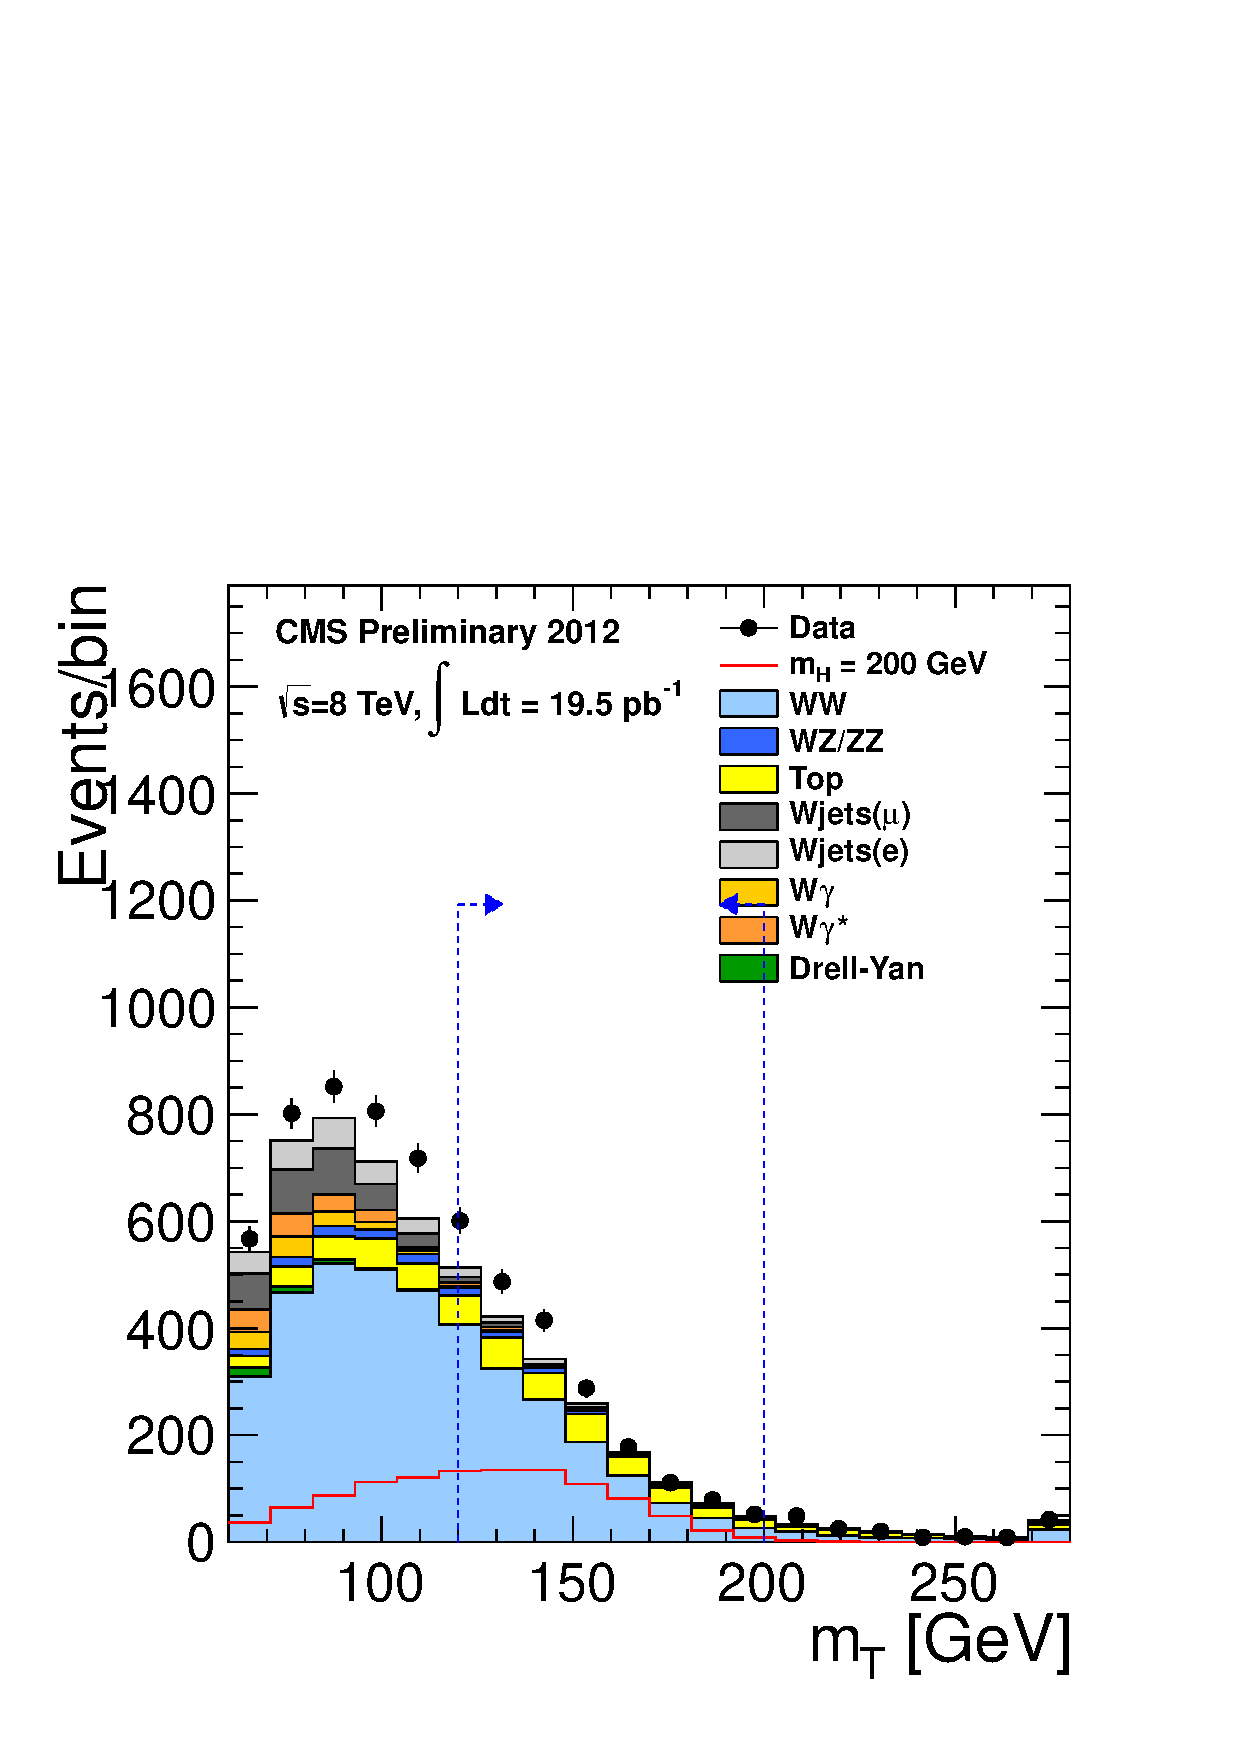
\includegraphics[width=0.45\textwidth]{figures/hww_analysis16_200_ALL_of_0j_mt.pdf}
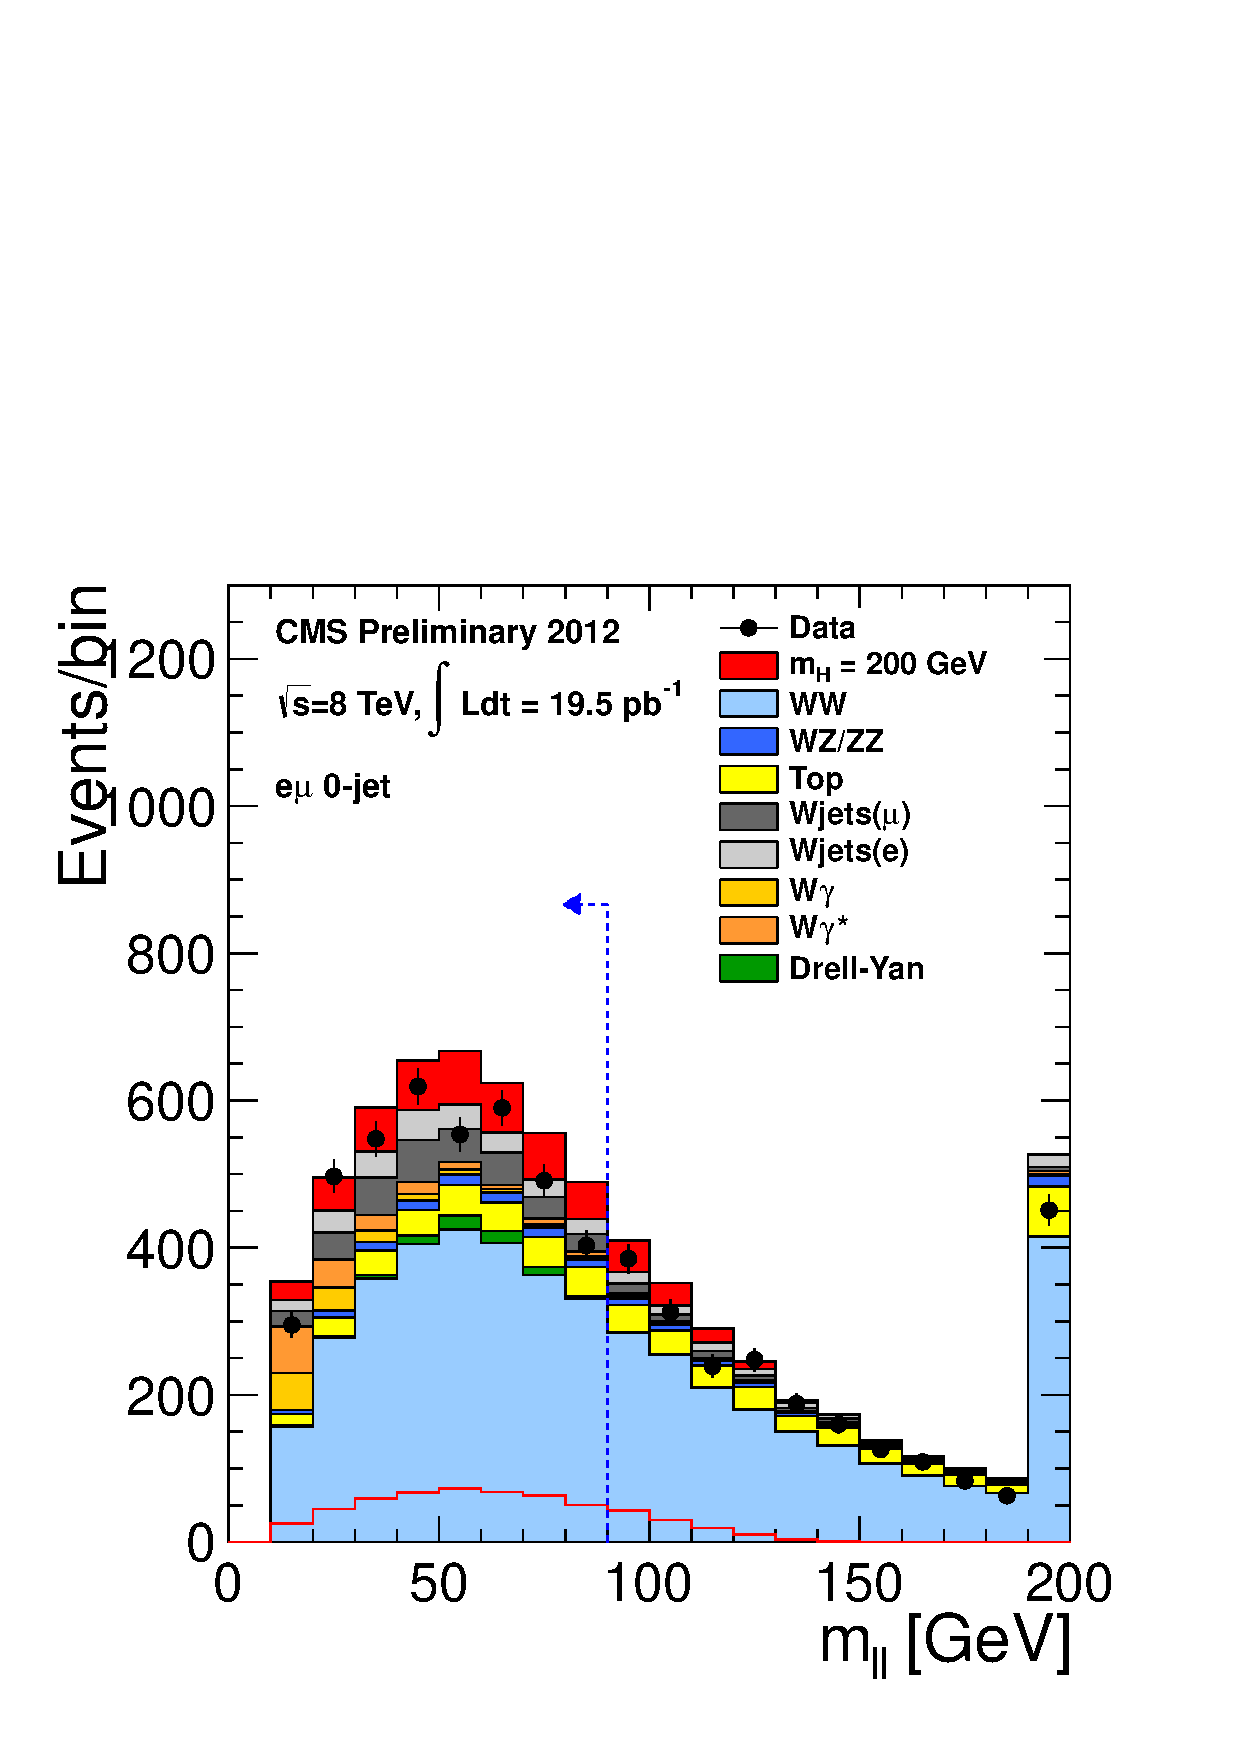
\includegraphics[width=0.45\textwidth]{figures/hww_analysis16_200_ALL_of_0j_mll.pdf}
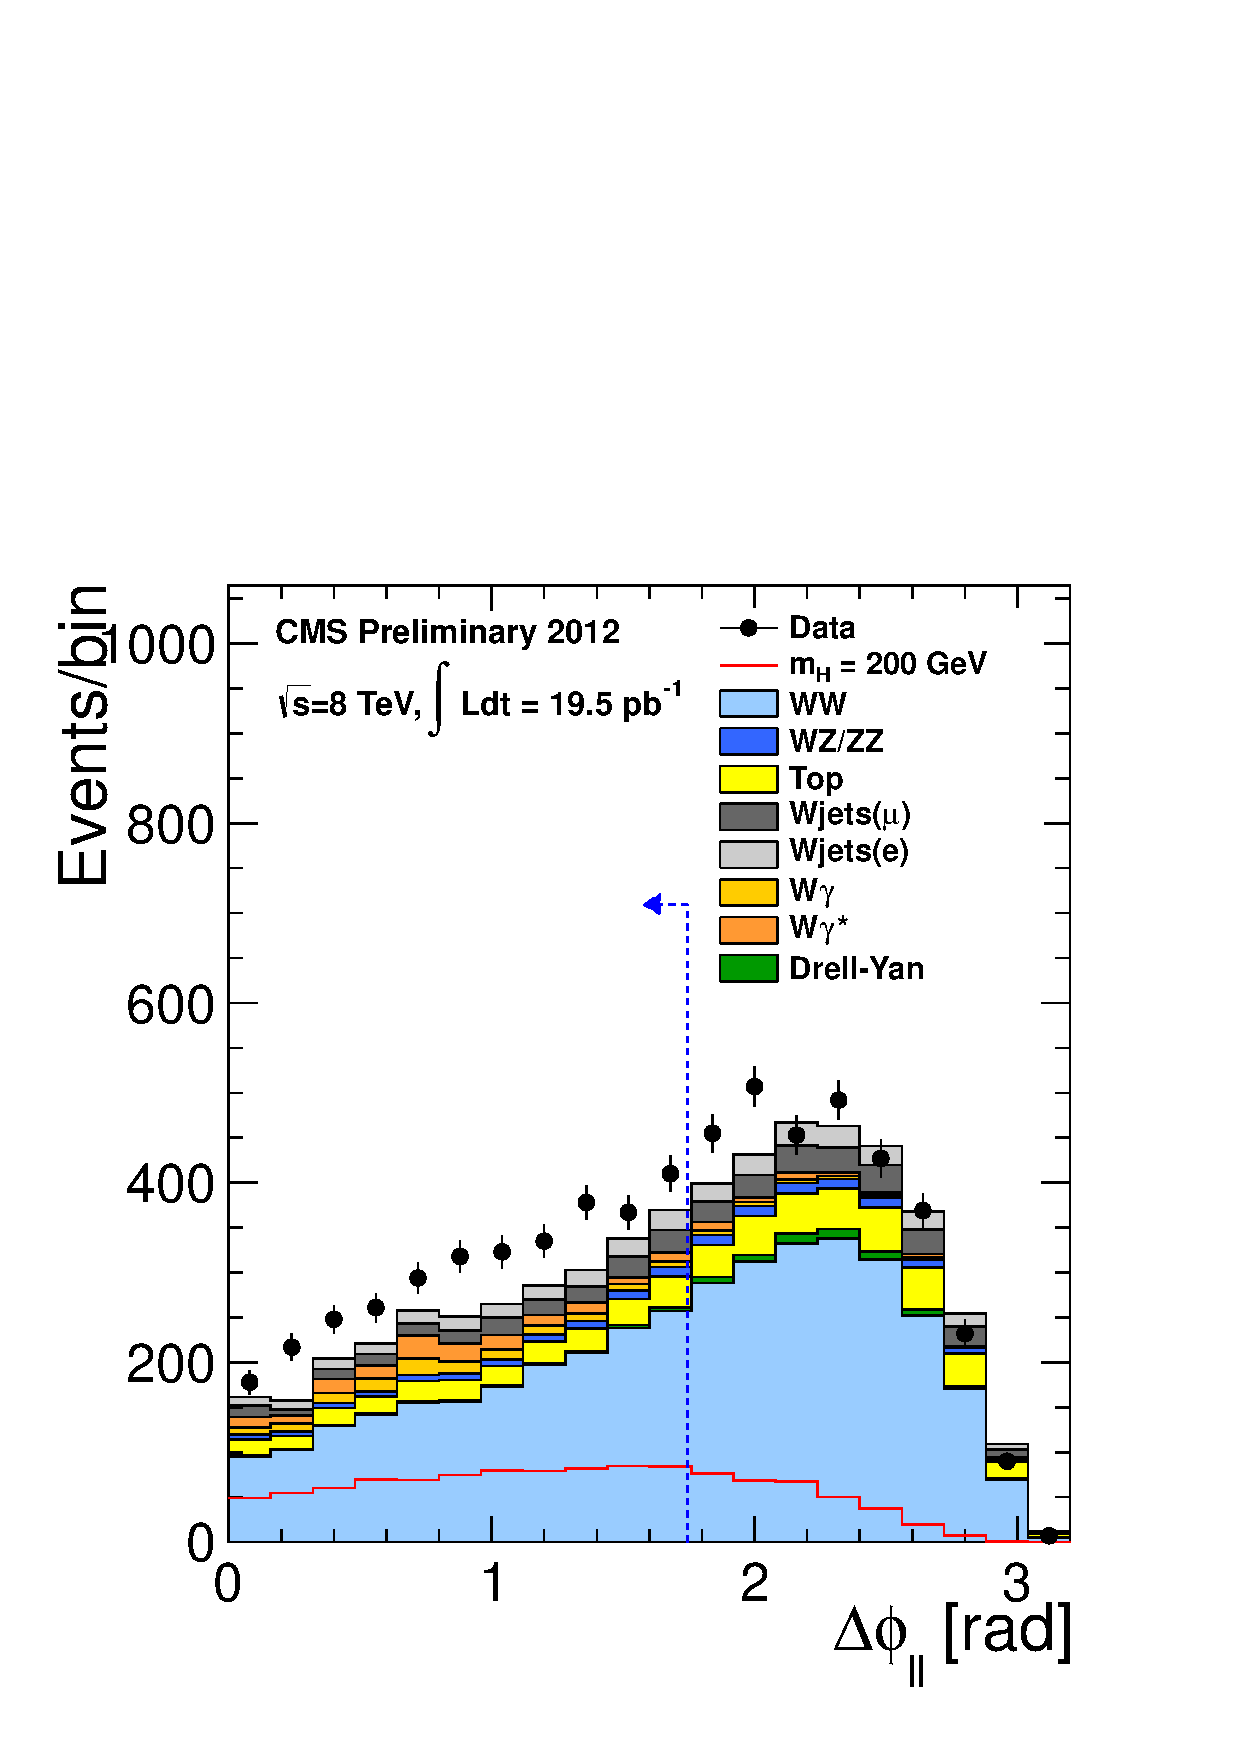
\includegraphics[width=0.45\textwidth]{figures/hww_analysis16_200_ALL_of_0j_dphi.pdf}
%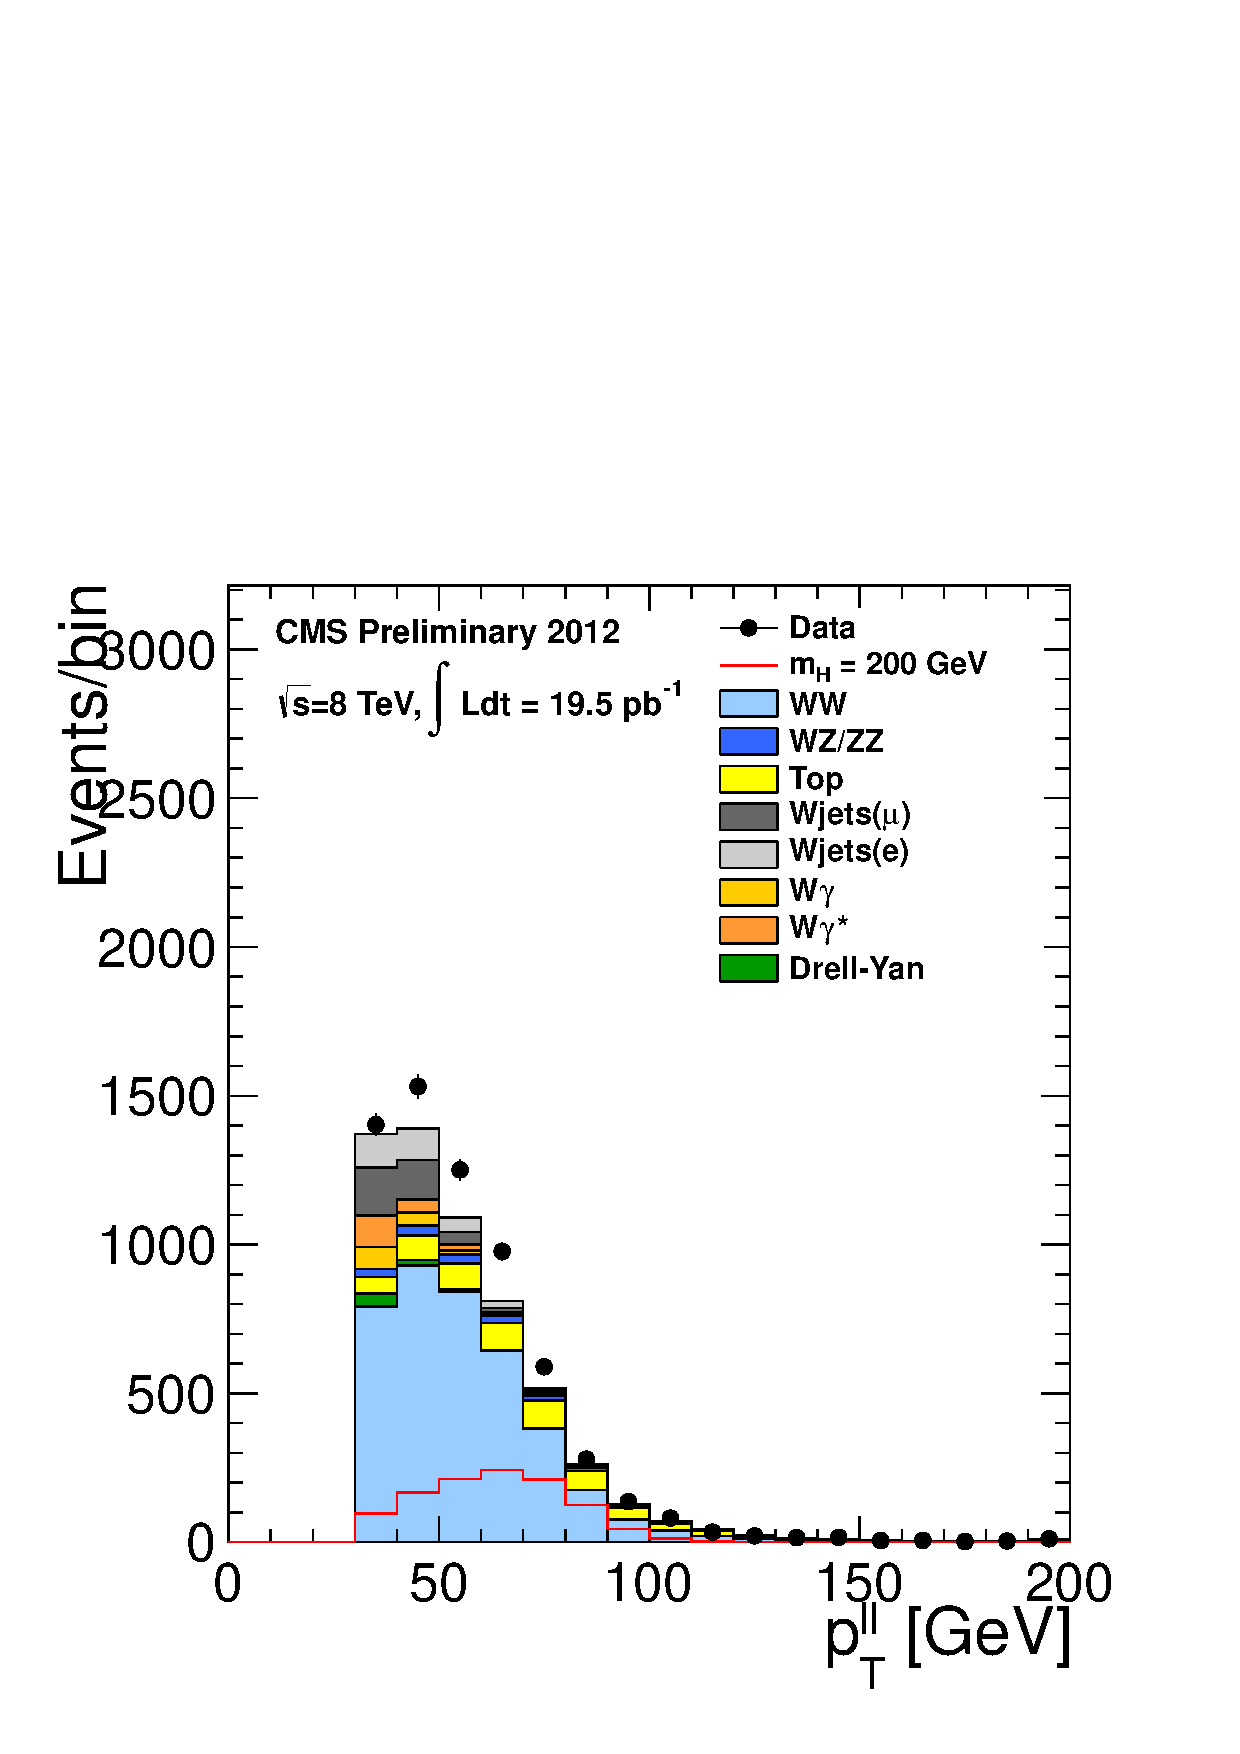
\includegraphics[width=0.45\textwidth]{figures/hww_analysis16_200_ALL_of_0j_ptll.pdf}
\caption{ WW-level plots in 0-jet \DF\ channel with \mHi=200~\GeV\ signal overlaid. 
Cuts for \mHi=200~\GeV\ is shown with blue dotted lines and arrows. 
}
\label{fig:wwlevelmh200}
\end{figure}

Figure~\ref{fig:wwlevelmh125}-\ref{fig:wwlevelmh200} show the signal and the background 
distributions of the five variables at WW-level for three \mHi\ hypotheses 
at 125, 160 and 200~\GeV. The signal is overlaid on the background, and   
the cut values are indicated on the plots.  
The cut values for all \mHi\ points studied by this analysis is 
shown in Table~\ref{tab:cutbasedtable}.
Applying these cuts, S/B is improved from 2 - 4~\% to 15 - 20~\%
depending on the categories. 

% --- WW 
% 0jet          1jet
% SF    DF      SF      DF
% 2676  6399    1465    3950    => bkg
% 84    237     26      95      => sig
% 3%    3.7%    1.8%    2.4%    => S/B

% --- cut-based 
% 0jet          1jet
% SF    DF      SF      DF
% 209   429     112     361 
% 37    88      16      55
% 18%   21%     14%     15%

%
\begin{table}[!ht]
  \begin{center}
  \small
  \vspace{0.5cm} 
  \caption{\mHi-dependent event selection for the cut-based analysis 
           in the 0-jet and 1-jet categories. }
  \vspace{0.5cm} 
  \begin{tabular} {|c|c|c|c|c|c|c|}
  \hline
\mHi~[\GeV] & \ptlmax~[\GeV] & \ptlmin~[\GeV] & \mll~[\GeV]   & \delphill~[$\cdot$] 
            & \mT~[\GeV] \\  
  \hline 
            &   $>$          &   $>$          &   $<$         &  $<$             
            &            \\  
  \hline \hline
    115 & 20  &  10     & 40  & 115 & 80 - 110  \\
    120 & 20  &  10     & 40  & 115 & 80 - 120  \\
    125 & 23  &  10     & 43  & 100 & 80 - 123  \\
    130 & 25  &  10     & 45  & 90  & 80 - 125  \\
    135 & 25  &  12     & 45  & 90  & 80 - 128  \\
    140 & 25  &  15   	& 45  & 90  & 80 - 130  \\
    145 & 25  &  15   	& 45  & 90  & 80 - 130  \\
    150 & 27  &  25   	& 50  & 90  & 80 - 150  \\
    160 & 30  &  25   	& 50  & 60  & 90 - 160  \\
    170 & 34  &  25   	& 50  & 60  & 110 - 170 \\
    180 & 36  &  25   	& 60  & 70  & 120 - 180 \\
    190 & 38  &  25   	& 80  & 90  & 120 - 190 \\
    200 & 40  &  25   	& 90  & 100 & 120 - 200 \\
    250 & 55  &  25   	& 150 & 140 & 120 - 250 \\
    300 & 70  &  25   	& 200 & 175 & 120 - 300 \\
    350 & 80  &  25   	& 250 & 175 & 120 - 350 \\
    400 & 90  &  25   	& 300 & 175 & 120 - 400 \\
    450 & 110 &  25   	& 350 & 175 & 120 - 450 \\
    500 & 120 &  25   	& 400 & 175 & 120 - 500 \\
    550 & 130 &  25   	& 450 & 175 & 120 - 550 \\
    600 & 140 &  25   	& 500 & 175 & 120 - 600 \\
  \hline
  \end{tabular}
  \label{tab:cutbasedtable}
  \end{center}
\end{table}






%%%%%%%%%%%%%%%%%%%%%%%%%%%%%%%%%%%%%%%
\section{Shape-based Method}
\label{sec:shape}
%\begin{itemize} 
%\item Motivation : easier interpretation, simpler implementation  
%\item applied to only $e\mu$ channel due to poor modeling of DY shape in $ee/\mu\mu$   
%\item Choice of variables : mass-like ones
%\item Binning: avoid poor stat, empty bins in bkgd templates. 
%      show relative statistics uncertainty of each bkgd. 
%      show S/B with different binning. 
%\item Range : show expected significance expanding range from signal region to the full 
%      [\mT, \mll] range $\rightarrow$ these are basically what's already in the 2D note 
%\item mention that there are two templates for low/high \mHi. 
%      additional selection($\ptlmax>50\GeV$) for high \mHi~templates
%\item now show 2D templates for selective \mHi~points(125,160,200,400) and each background process
%      (Show 8TeV 0jet only. The rest will be in the appendix)
%\item Technicality : unrolling  procedure. show some unrolled templates and mention that 
%      these are what's actually used by Stat machineries. mention correlation is still there. 
%\end{itemize}  

The ``shape-based method" uses binned 2-dimensional templates of \mT\ and \mll. 
This method is more complicated than the cut-based method
because it uses the shape and the additional uncertainties to the shape 
on top of normalization should be taken into account. 
To extract the signal component, the 2-dimensional binned shape is fitted to data. 
The shapes for most of the background are taken from simulation except 
the \Wjets\ which is taken from data subtracted by simulation. 
Therefore, it is critical to make sure that the fit model correctly describes 
what is observed in data. There was a huge effort to validate this using 
pseudo-data and data-control region. Chapter~\ref{ch:fit_validation} describes 
the details. 

There are two main motivations for developing this analysis method. 
Before this method was employed as the main analysis method for the 
public result of this analysis at CMS, the BDT-based multivariate method 
had been the main analysis method~\cite{CMS-PAS-HIG-12-038}. However, because of 
the non-trivial dependence of the discriminator(BDT score)
on the input variables, it was very difficult to have a
physical interpretation of the observed result with this method. 
For example, if there is a fluctuation in data, we do not know where this comes from, 
\textit{i.e.} which input variable is responsible for this unexpected 
behavior. In addition, because a single template definition is used for multiple 
\mHi\ hypotheses, it avoids unnecessary statistical fluctuations between data selected 
for adjacent hypotheses.
On the practical side, the implementation of the 
analysis became much simpler compared to the BDT method because of using 
the same background template across different \mHi\ hypotheses
while the BDT method used \mHi-dependent selection similar to the cut-based 
method. This not only simplified the work flow but also allowed to draw 
the 2-dimensional log likelihood scan in the plane of 
signal strength and \mHi, which was not possible with the \mHi-dependent 
selections for some technical reasons. 

The modeling of \met\ in \dyll\ background is quite poor in the tail of high \met. 
This is because high \met\ in this process can be obtained when jet energy is 
poorly measured. This corresponds to the tail of jet energy response distribution 
which is not well modelled by a Gaussian function which is used to estimate the 
resolution in the bulk of the distribution. Given that the Monte Carlo simulation 
is based on random sampling, this part is not particularly well modelled. 
In addition, the statistics of the available MC sample is limited resulting in huge weights
per event. Therefore, we can not rely on \dyll\ simulation, and  
the shape-based method is applied to only \DF\ channels. 

The choice of the variables is motivated by the fact that the best 
variable that discriminates signal from background is the Higgs mass. 
But, due to the neutrinos in the final state, the Higgs mass can not be 
reconstructed. Therefore, we use the two \mHi-like variables, 
the Higgs transverse mass(\mT) and the di-lepton mass(\mll)
to construct the 2-dimensional templates. These two variables are 
weakly correlated in the main background processes.
%\textcolor{red}{why strong correlation for \wgamma, \wgammastar?} 
%allowing maximum advantage of using two variables.  
%\textcolor{blue}{show bin-normalized templates for 125/160/250 and qqww 
%and mention that signal vs. qqww, signal vs. signal(data should be able to 
%distinguish different hypotheses) comparison}
\begin{figure}[htp]
\centering
\subfigure[$\mHi=125~\GeV$]{
\centering
\label{subfig:2dNormBin_mH125}
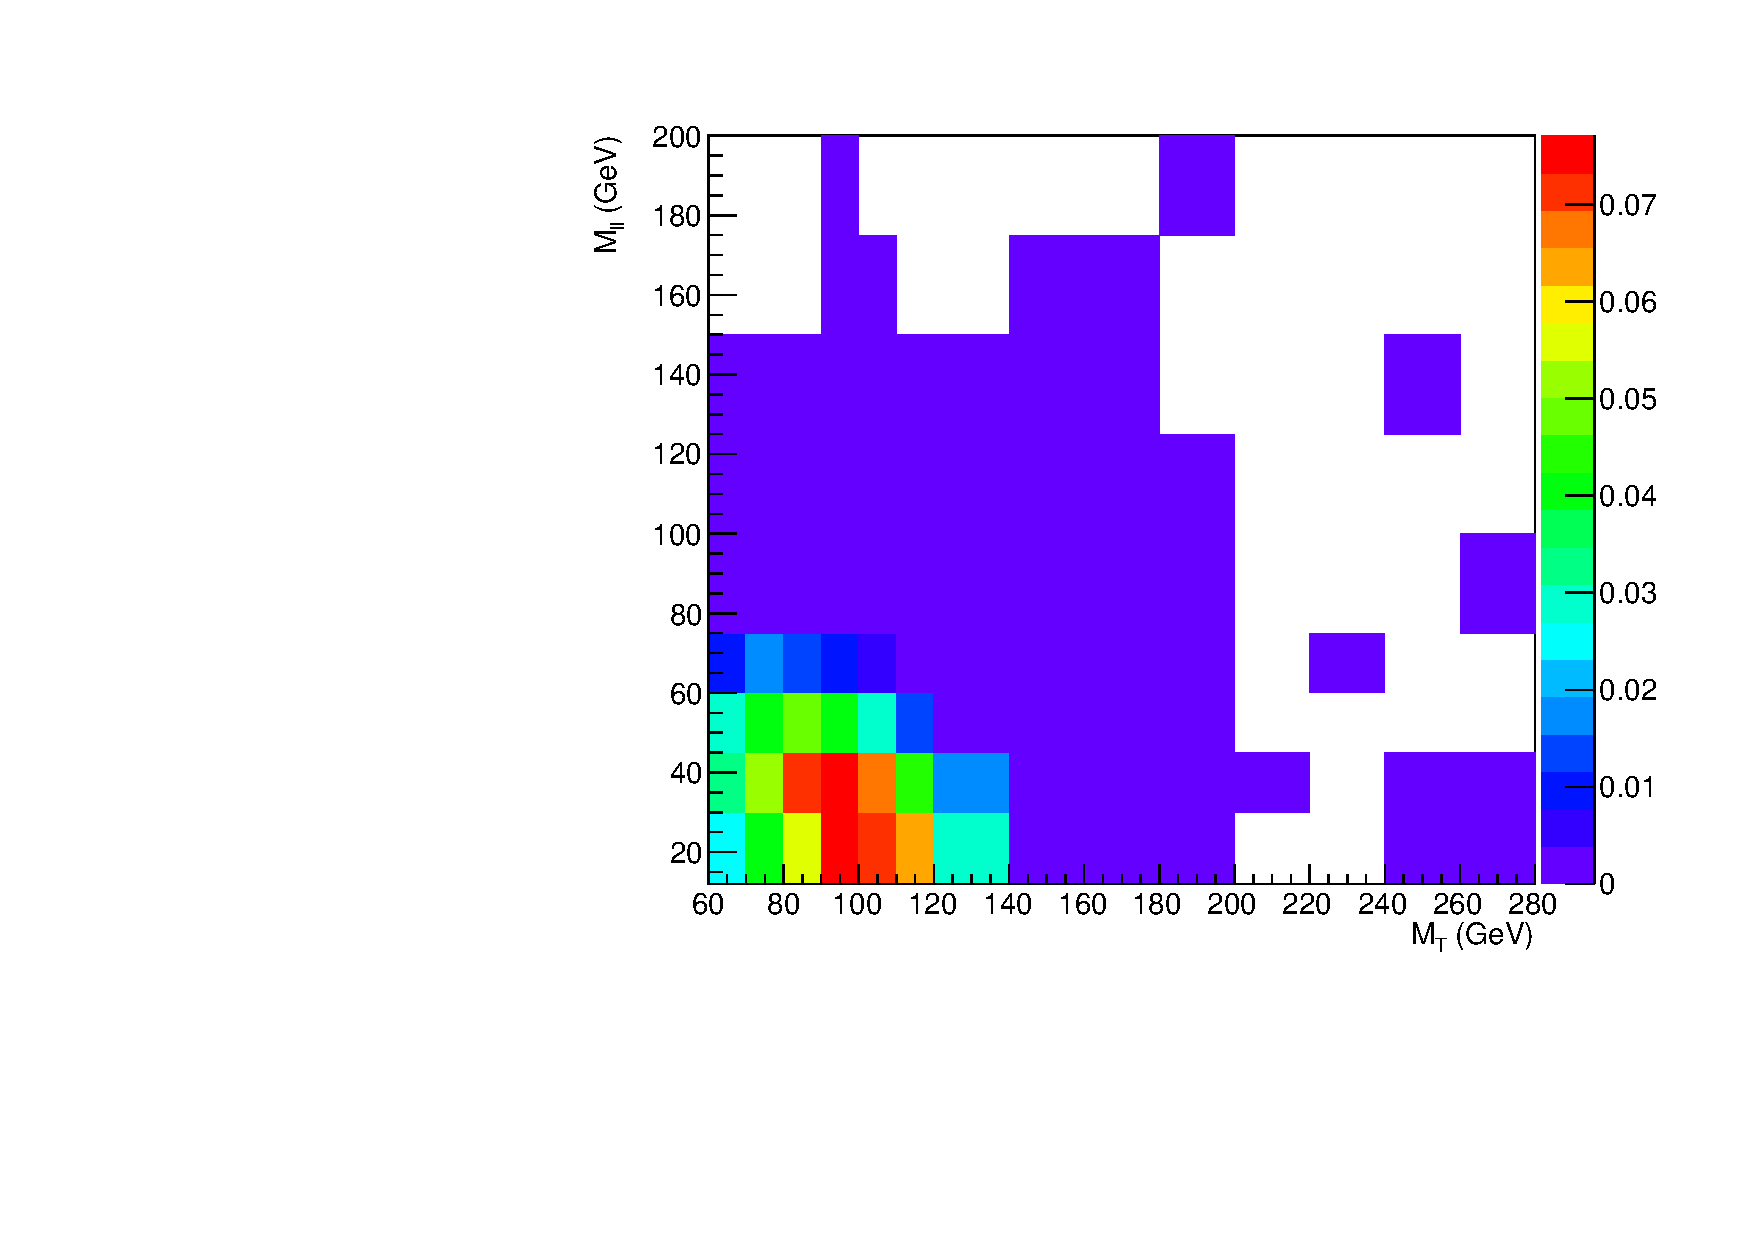
\includegraphics[width=0.45\textwidth]{figures/2dNormBin_mH125.pdf}
}
\subfigure[$\mHi=160~\GeV$]{
\centering
\label{subfig:2dNormBin_mH160}
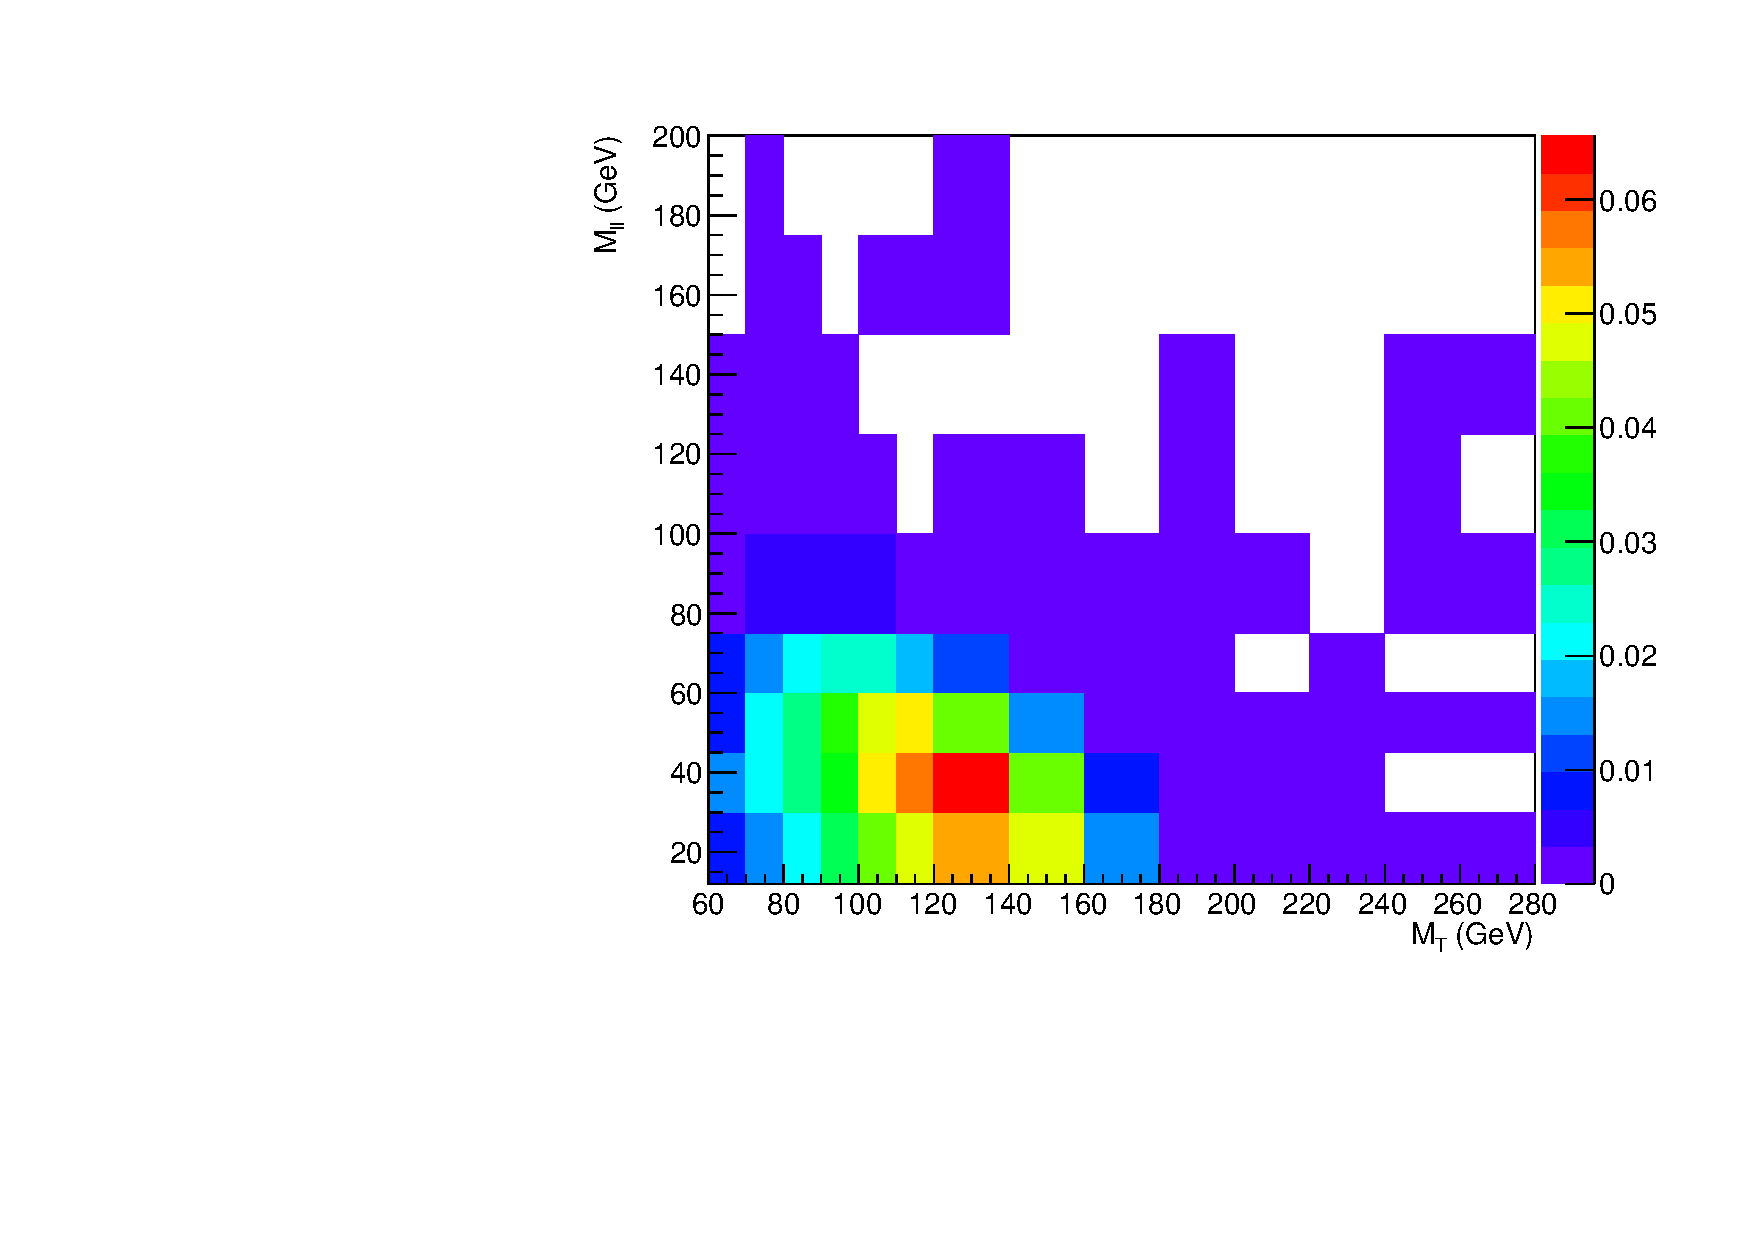
\includegraphics[width=0.45\textwidth]{figures/2dNormBin_mH160.pdf}
}
\subfigure[$\mHi=200~\GeV$]{
\centering
\label{subfig:2dNormBin_mH200}
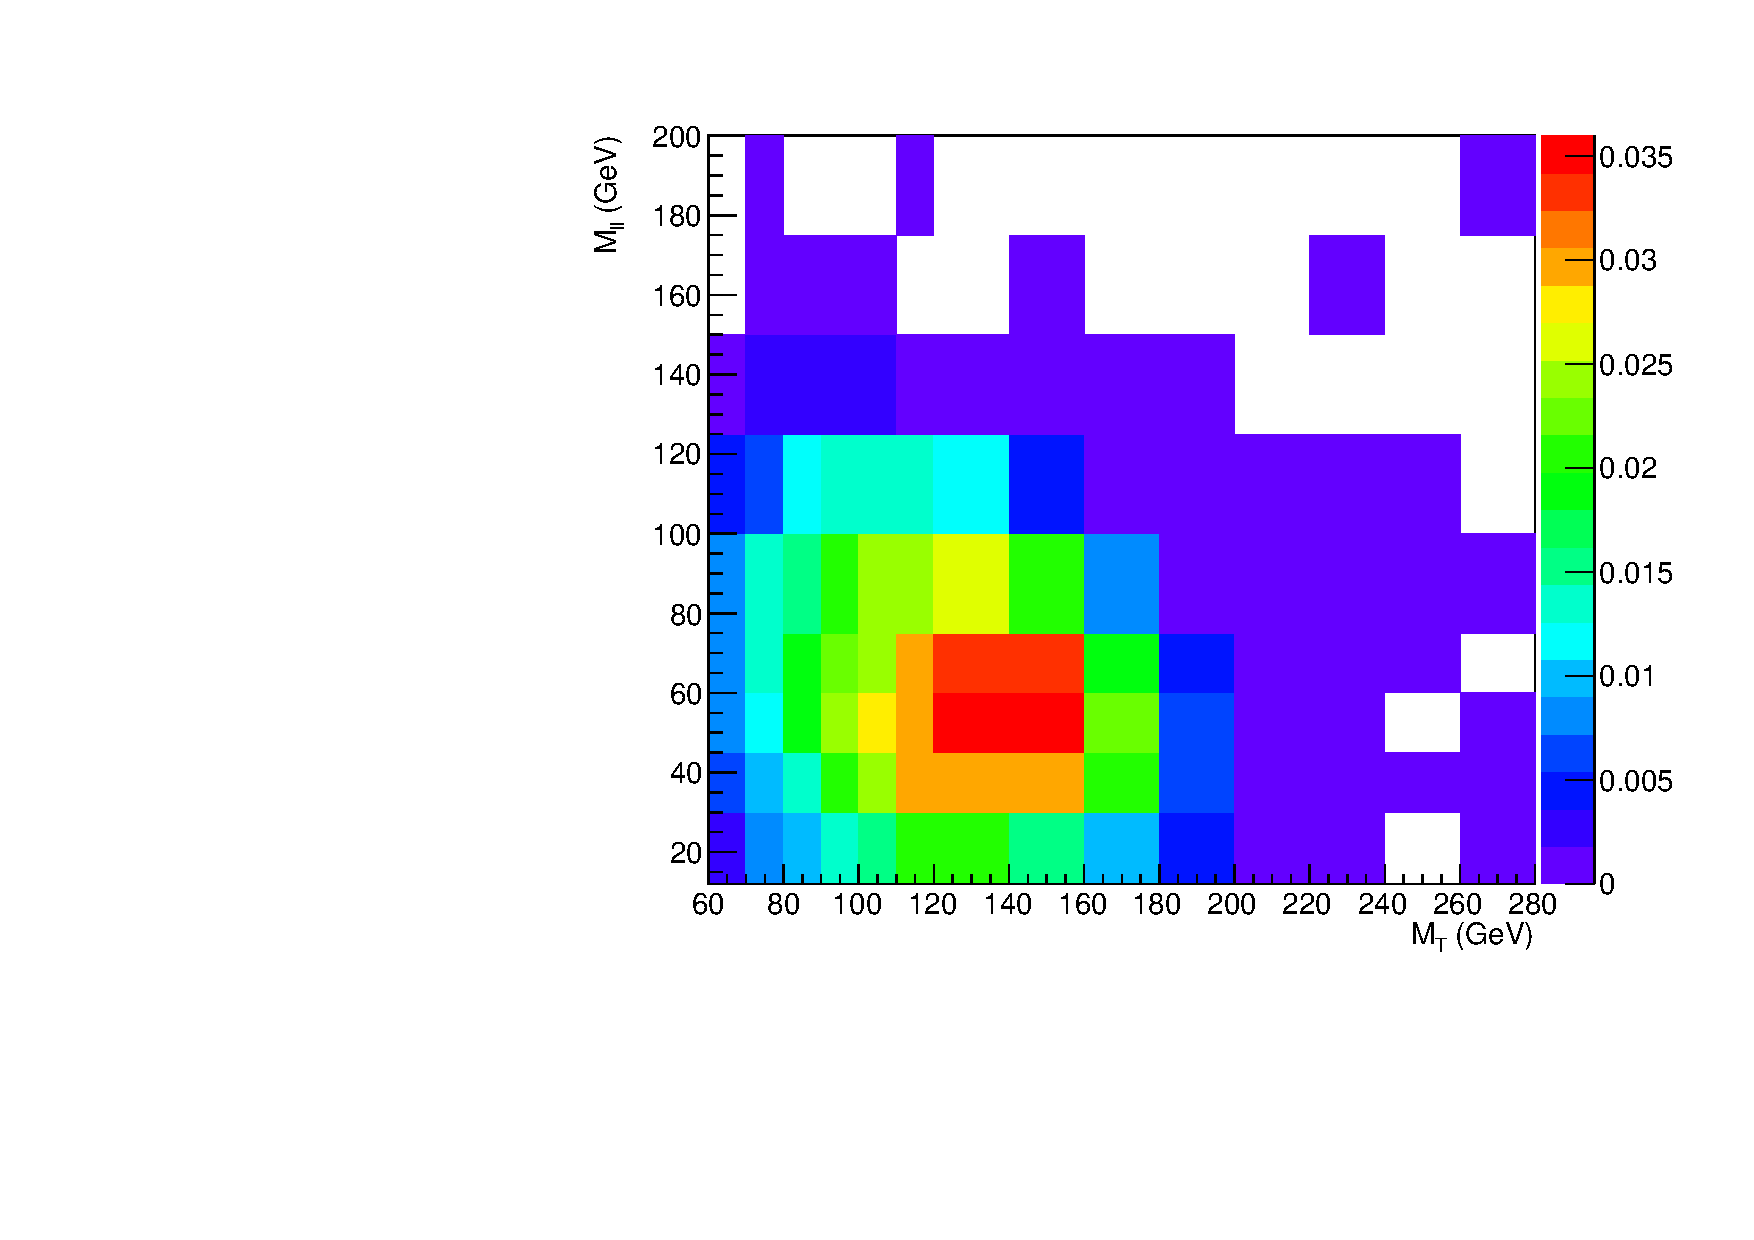
\includegraphics[width=0.45\textwidth]{figures/2dNormBin_mH200.pdf}
}
\subfigure[\qqww]{
\centering
\label{subfig:2dNormBin_qqWW}
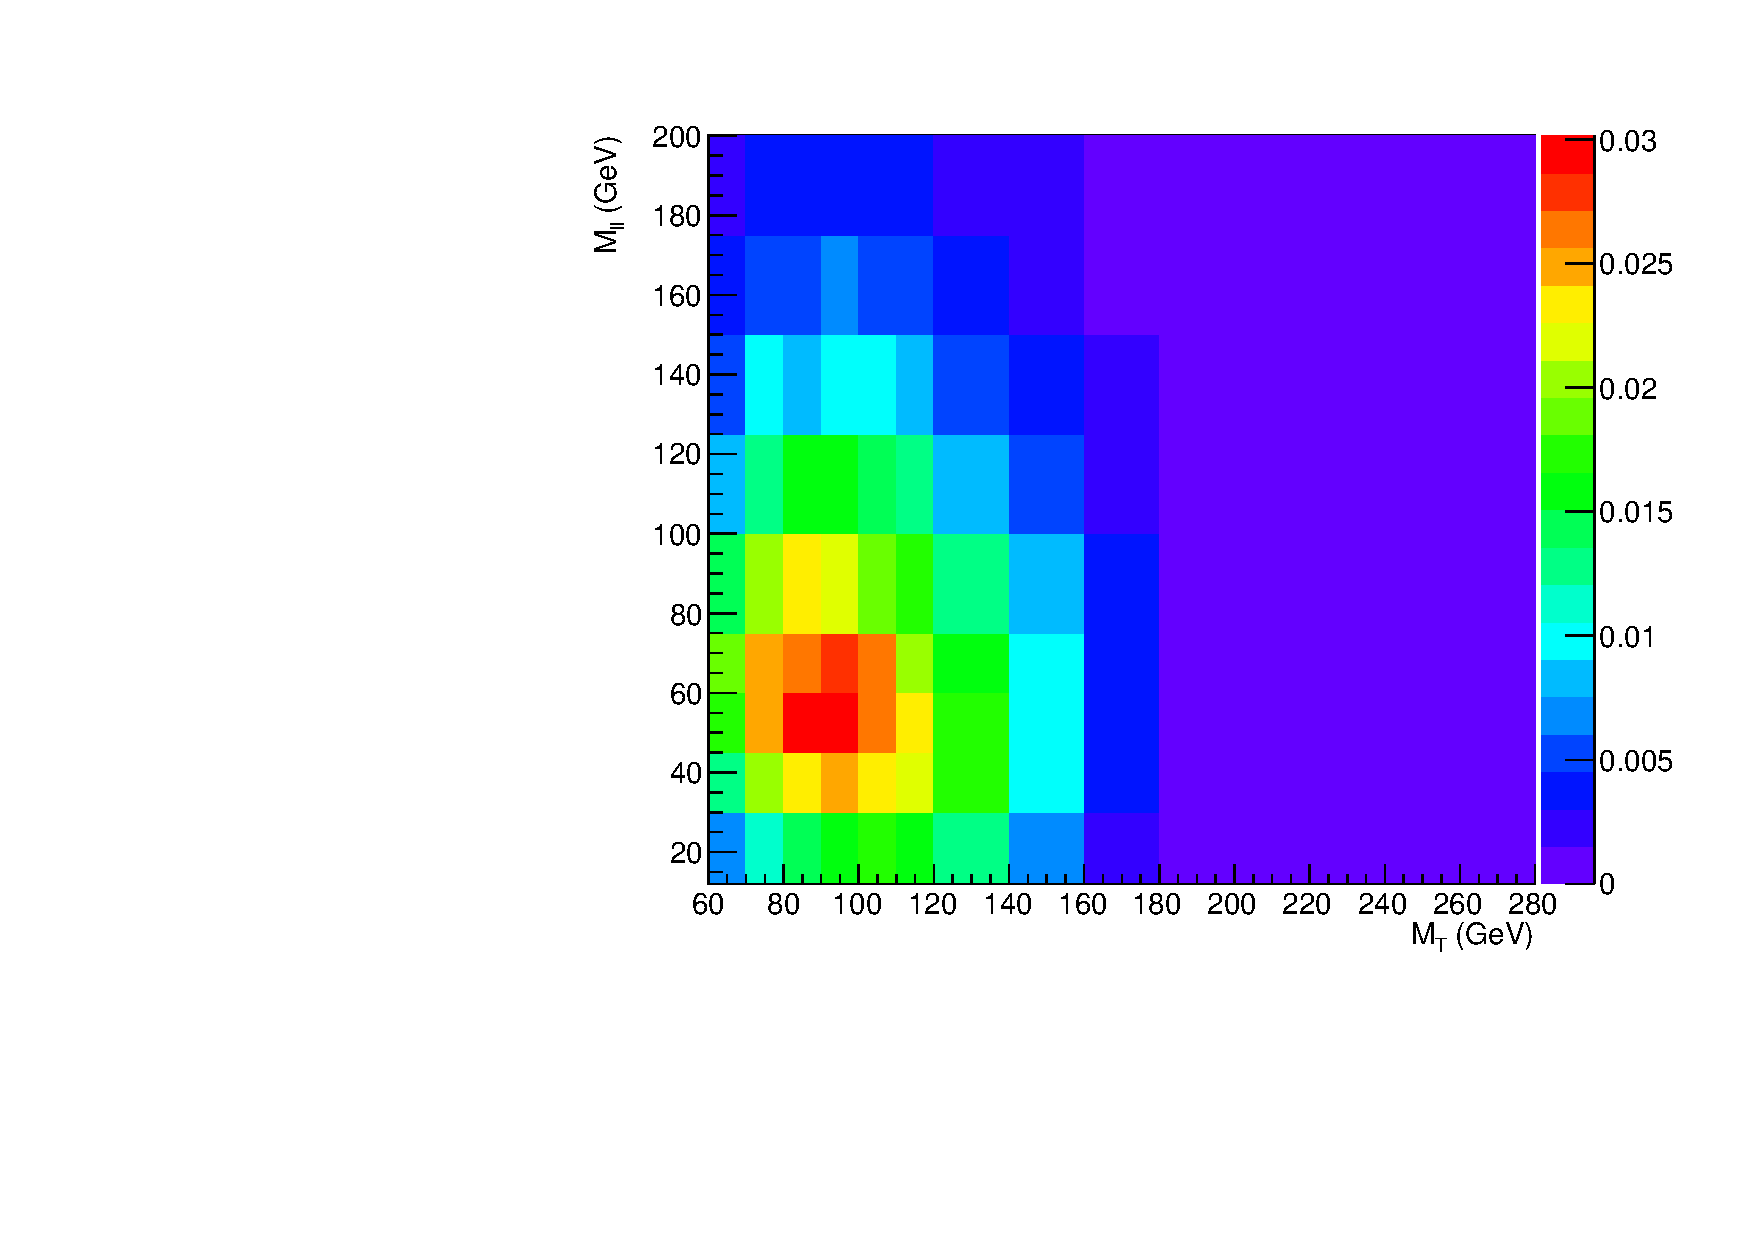
\includegraphics[width=0.45\textwidth]{figures/2dNormBin_qqWW.pdf}
}
\caption{ 2D templates for $\mHi=125, 160, 200~\GeV$ and \qqww. 
For visualization, each bin is divided by 
the area of the bin in order to avoid random peaks due to difference in the bin size.  
}
\label{fig:2dNormBin}
\end{figure}


For the determination of the range and the binning, following points were considered : 
\begin{itemize}
\item Range should cover multiple \mHi
\item Binning should allow enough granularity to distinguish the signal from the background 
      in the region where signal is populated : sideband region can have coarser binning 
      in case of low statistics in that region
\item statistical uncertainty of the templates should be small with respect to the 
      total background : otherwise the templates will not be reliable  
\item There should not be any empty bin when all backgrounds are summed : otherwise any excess 
      in data will claim infinite significance, \textit{i.e.} something is observed when nothing 
      expected
\item The data events in the bins should be reasonably populated so that the nuisances 
      can be constrained by data
\end{itemize}

Due to large difference in the kinematics of signal events between high and low \mHi, 
we decided to use two template definitions, one for the low Higgs masses, 
\mHi = 110 - 250~\GeV, and the other for the high Higgs masses, \mHi = 300 - 600~\GeV. 
In order to further enhance S/B, $\ptlmax>50~\GeV$ is applied for the 
high \mHi\ templates. 
So, for the low(high) \mHi\ hypotheses, we use 
$60 < \mT < 280~\GeV$($60 < \mT < 380~\GeV$)
and 
$0 < \mll < 280~\GeV$($0 < \mll < 450~\GeV$).
The events with high \mHi\ hypothesis tend to have high \mT\ and high \mll\, 
but this is the phase space where background processes are not populated. 
Thus, for the high \mHi\ templates, the top and the right bins are overflow bins 
allowing events up to $\mll<600~\GeV$ and $\mT<600~\GeV$, 
which covers \mHi\ hypothesis up to 600~\GeV.

The width of the \mT\ and \mll\ distribution in signal events 
is 20 - 25 \GeV\ for low \mHi\ events,
%\footnote{At WW level, \mT\ resolution in the 0-jet(1-jet) category is 20(25)~\GeV\ 
%for \mHi = 125~\GeV. The \mll\ resolution is 20~\GeV\ in both 0-jet(1-jet) category.}, 
so we take 20-25~\GeV as a maximum size of a bin for low \mHi\ templates.   
\begin{figure}[htp]
\centering
\subfigure[$\mT=10~\GeV, \mll=10~\GeV$]{
\centering
\label{subfig:SoverB_2d_10_10}
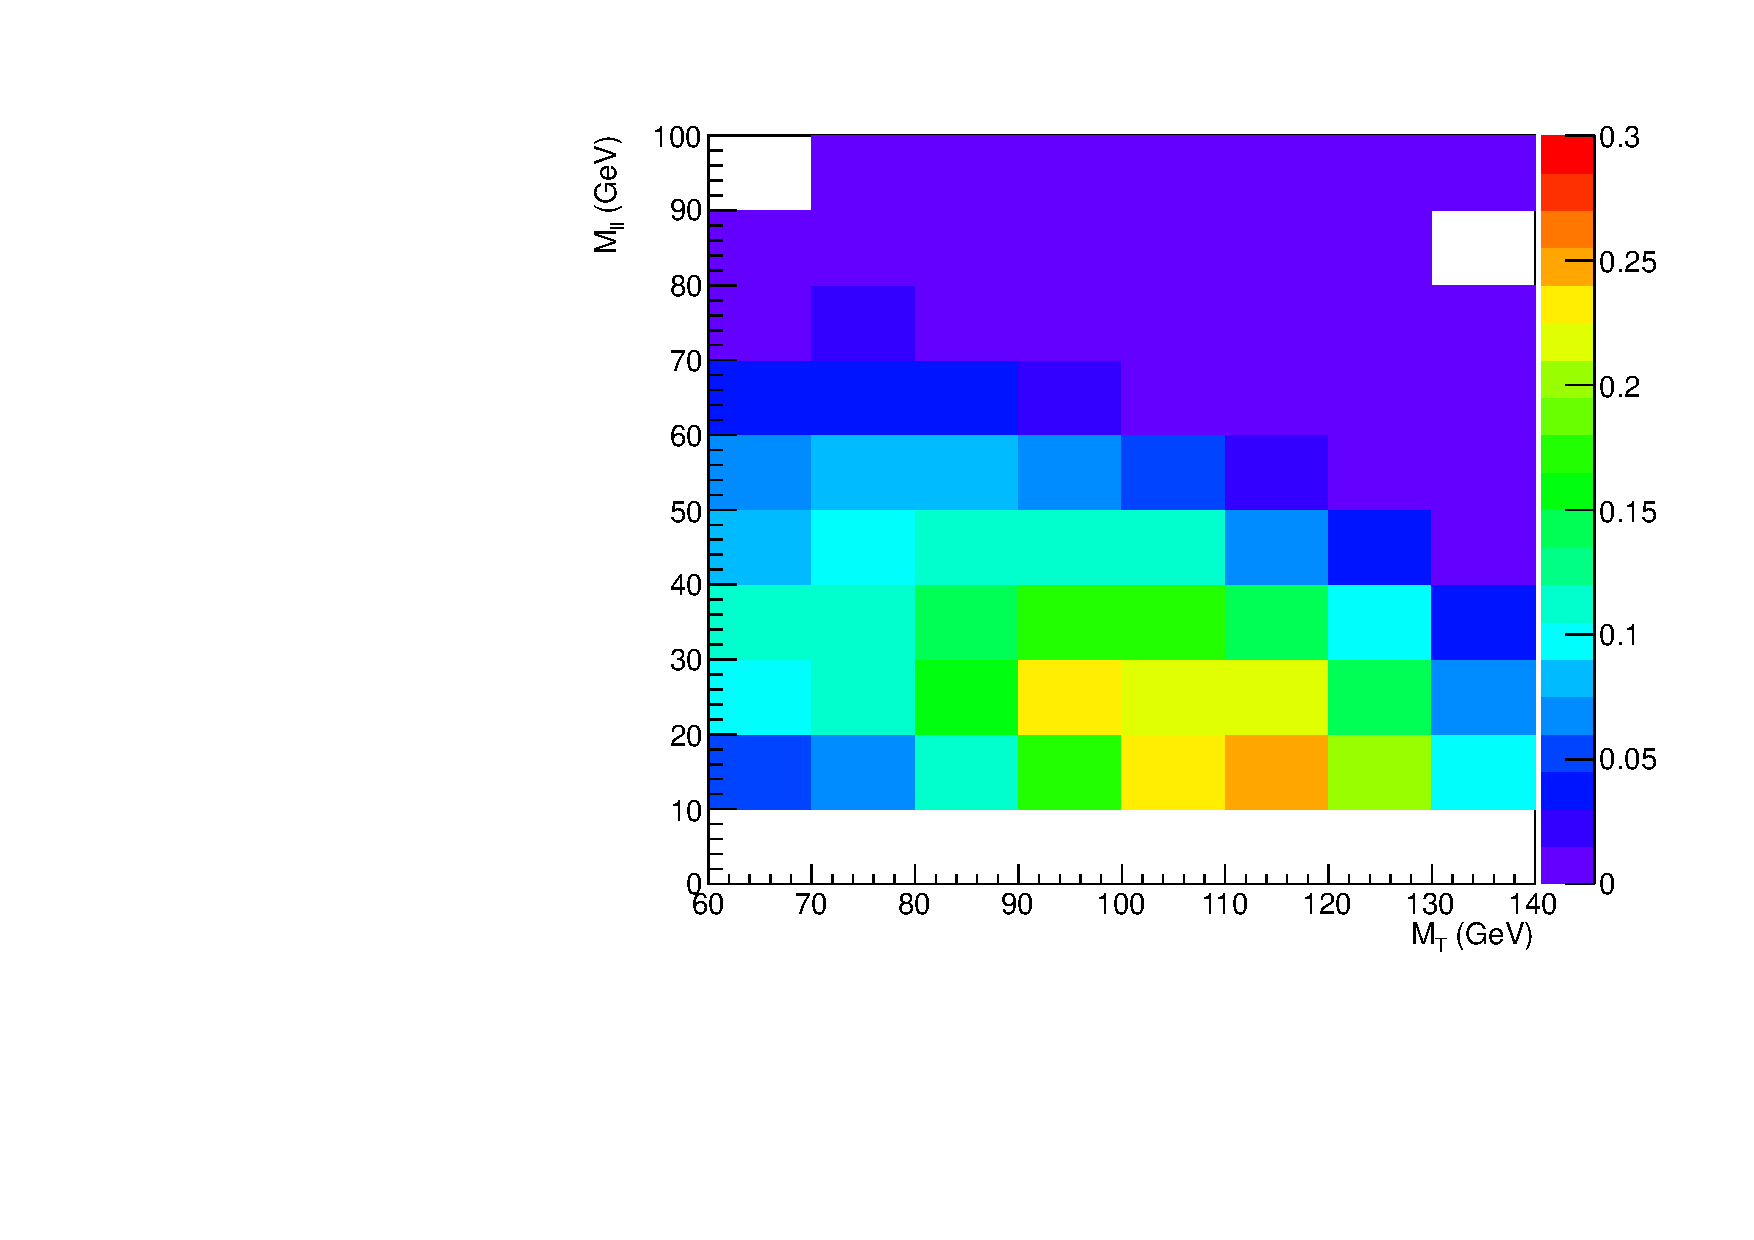
\includegraphics[width=0.45\textwidth]{figures/SoverB_2d_10_10.pdf}
}
\subfigure[$\mT=20~\GeV, \mll=10~\GeV$]{
\centering
\label{subfig:SoverB_2d_20_10}
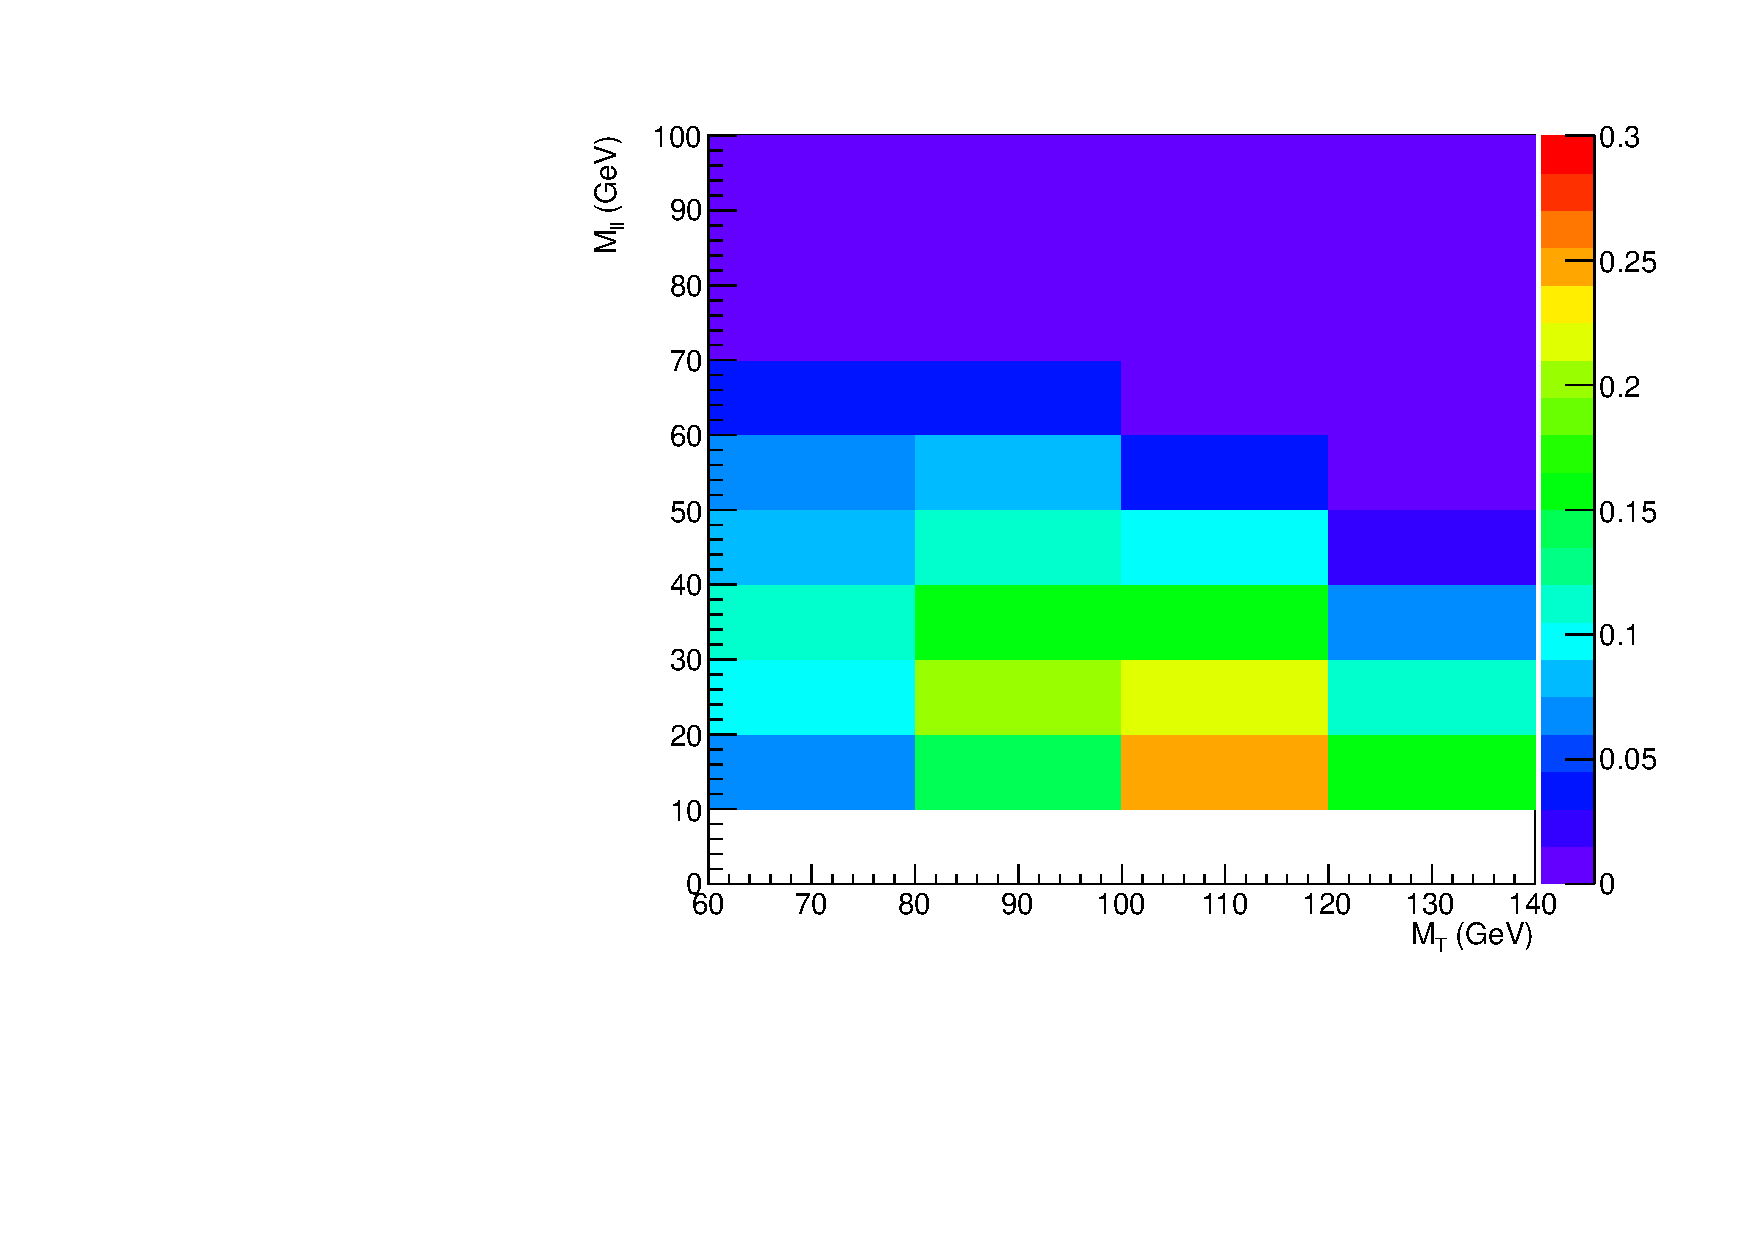
\includegraphics[width=0.45\textwidth]{figures/SoverB_2d_20_10.pdf}
}
\subfigure[$\mT=10~\GeV, \mll=20~\GeV$]{
\centering
\label{subfig:SoverB_2d_10_25}
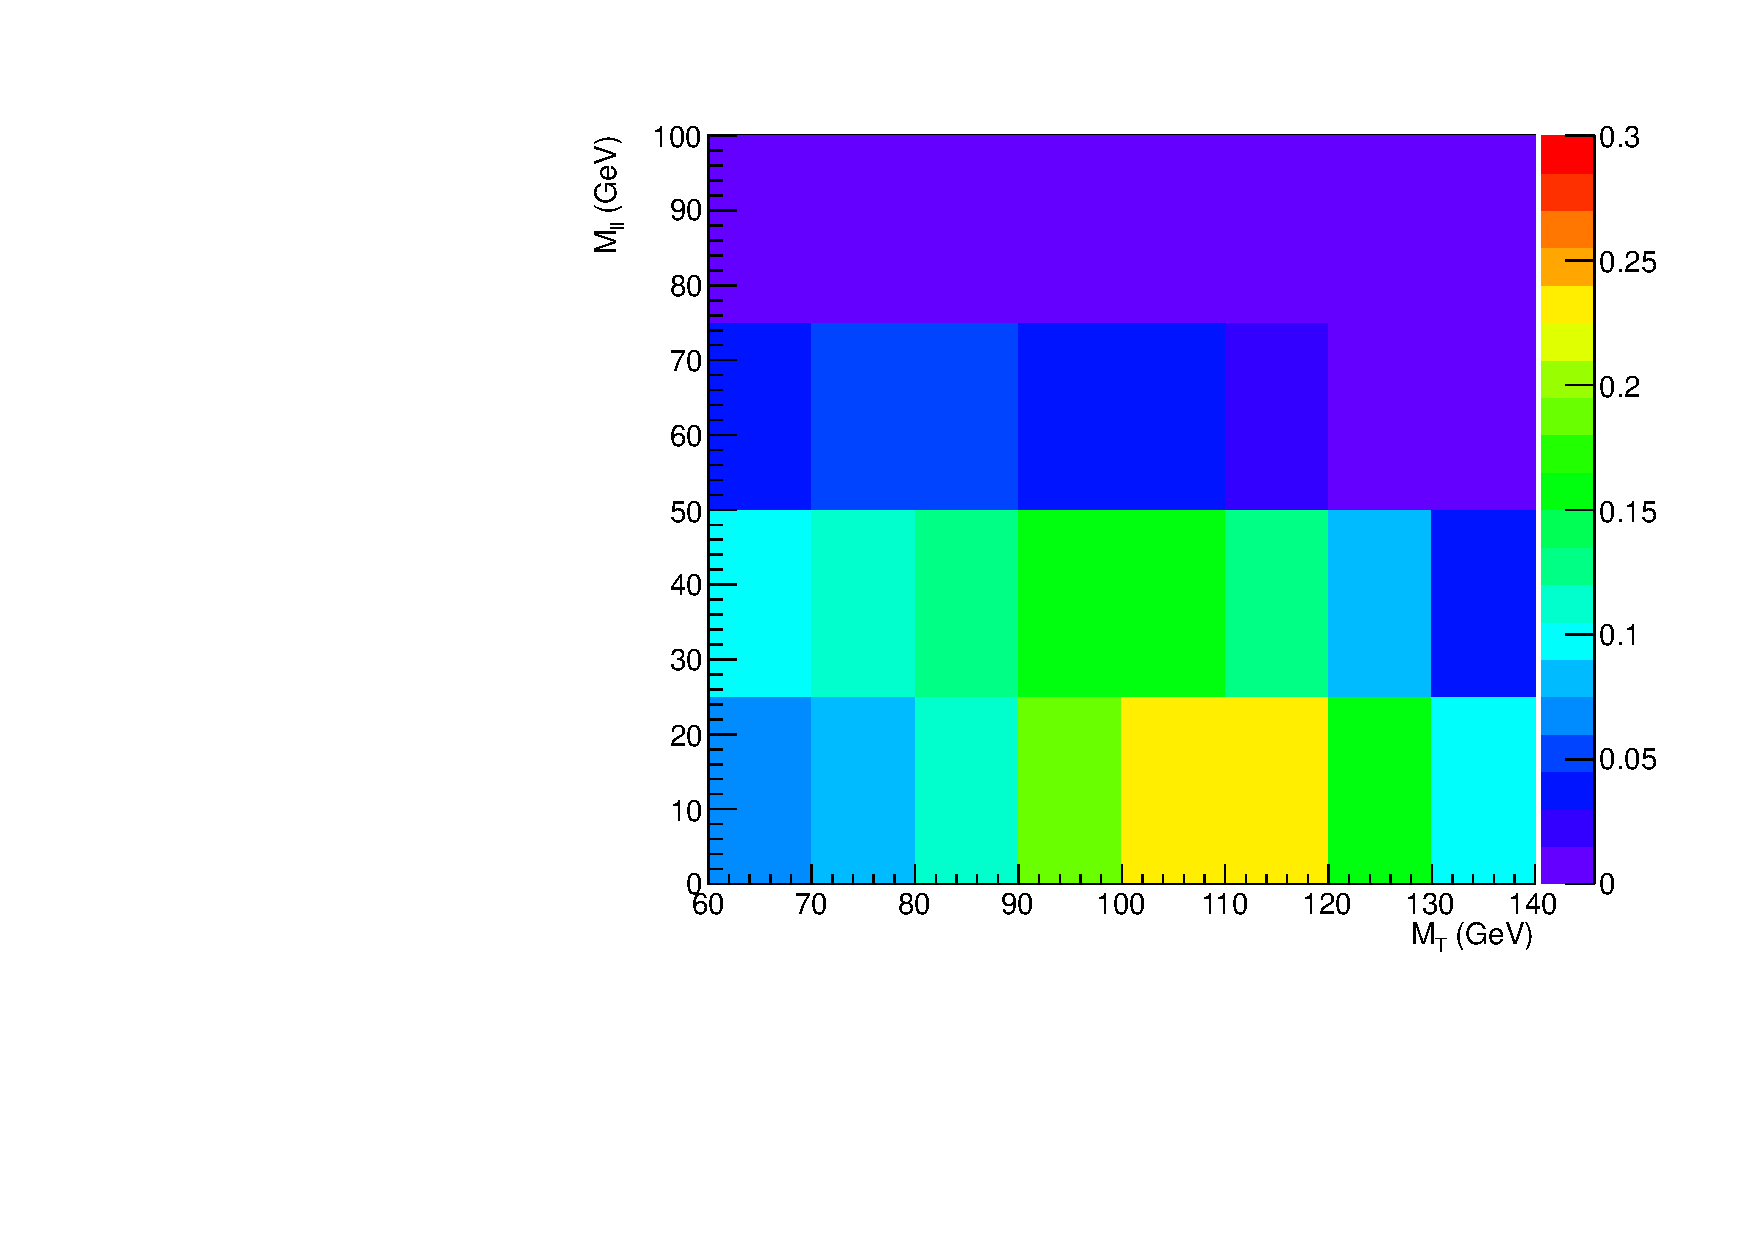
\includegraphics[width=0.45\textwidth]{figures/SoverB_2d_10_25.pdf}
}
\subfigure[$\mT=20~\GeV, \mll=25~\GeV$]{
\centering
\label{subfig:SoverB_2d_20_25}
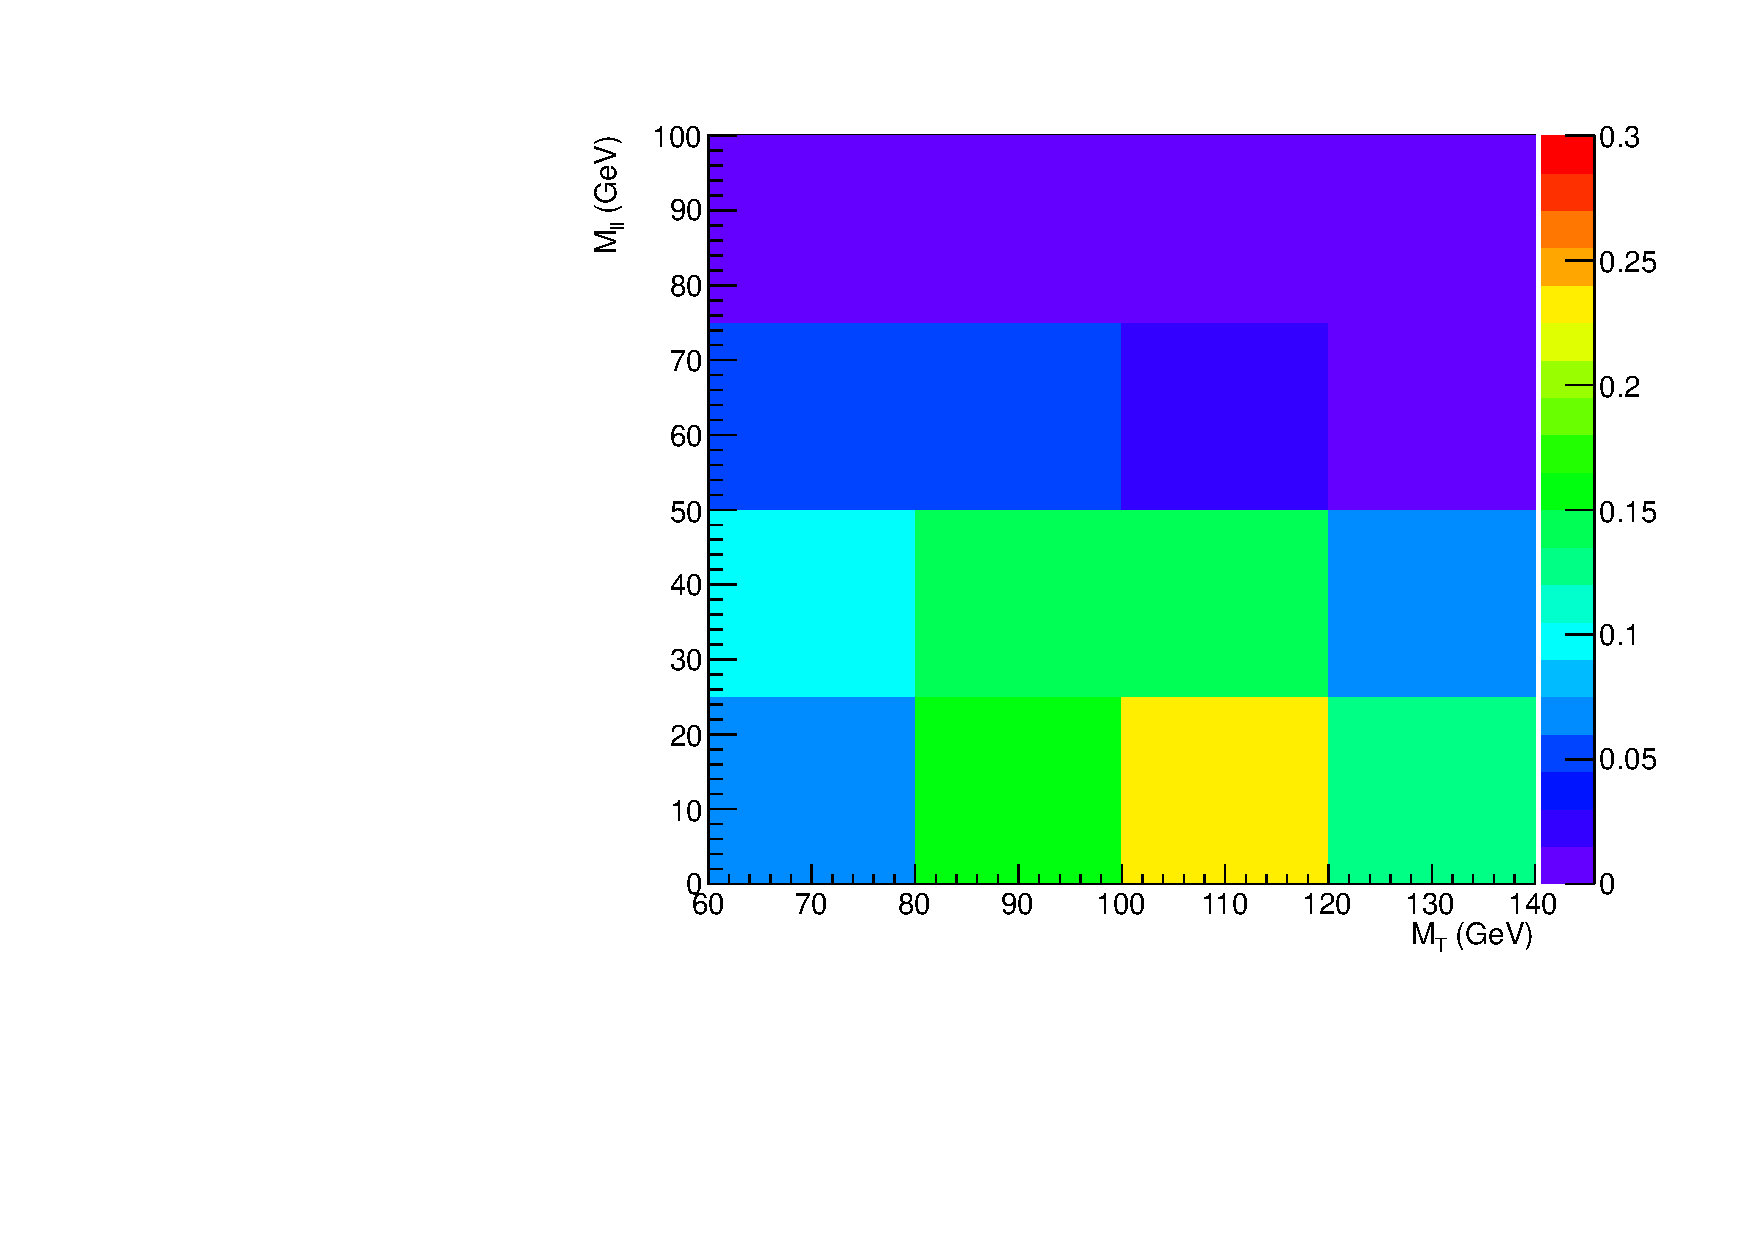
\includegraphics[width=0.45\textwidth]{figures/SoverB_2d_20_25.pdf}
}
\caption{ S/B using different binnings.   
The region($60<\mT<120~\GeV$, $0<\mll<100~\GeV$) is shown.}
\label{fig:SoverBdiffbinning}
\end{figure}
Figure~\ref{fig:SoverBdiffbinning} shows the S/B with 4 different binnings
in the region where \mHi=125~\GeV\ signal is populated($60<\mT<120~\GeV$, $0<\mll<100~\GeV$)
in the 0-jet \DF category ;
bin size of [\mT, \mll]  = [10~\GeV, 10~\GeV], [20~\GeV, 10~\GeV], 
[10~\GeV, 20~\GeV], and [20~\GeV, 20~\GeV]. 
The S/B with the bin size of 10 - 20~\GeV\ does not change S/B, 
so we can use any bin size in that range as long as each bin
contains enough statistics. 

\begin{table}[htp] 
\begin{center} 
\small
\vspace{0.5cm}
\caption{Expected significance with different binnings and range combinations. 
The result is from 0-jet \DF\ with 12.1 \ifb of data. As a reference, the expected 
significance from the BDT method is 1.80.} 
\vspace{0.5cm}
\begin{tabular}{c|c|c||c|c|c} 
\hline
binning & range & expected & binning & range & expected  \\
$\mT \times \mll$ & [\GeV]  & significance & $\mT \times \mll$ & [\GeV] & significance  \\
\hline \hline
\multirow{2}{*}{$2\times2$} & \mT\ : 80 - 125 & \multirow{2}{*}{1.76} &  
\multirow{2}{*}{$2\times4$} & \mT\ : 80 - 120 & \multirow{2}{*}{1.89}  \\
                            & \mll\ : 12 - 80 &  &  
                            & \mll\ : 0 - 100 &   \\
\hline
\multirow{2}{*}{$3\times3$} & \mT\ : 80 - 125 & \multirow{2}{*}{1.85} &  
\multirow{2}{*}{$5\times4$} & \mT\ : 80 - 180 & \multirow{2}{*}{2.06}  \\
                            & \mll\ : 12 - 80 &  &  
                            & \mll\ : 0 - 100 &   \\
\hline
\multirow{2}{*}{$4\times4$} & \mT\ : 80 - 125 & \multirow{2}{*}{1.88} &  
\multirow{2}{*}{$8\times6$} & \mT\ : 80 - 240 & \multirow{2}{*}{2.19}  \\
                            & \mll\ : 12 - 80 &  &  
                            & \mll\ : 0 - 150 &   \\
\hline
\end{tabular} 
\label{tab:2dbinningrangetest} 
\end{center} 
\end{table} 

This method gives about 25~\% better sensitivity at \mHi=125~\GeV\ 
in terms of expected significance compared to the state-of-the-art 
analysis method(BDT method)~\cite{CMS-PAS-HIG-12-038} when this method was developed. 
The improvement comes from using expanded phase space 
which can be used to constrain backgrounds further. 
Table~\ref{tab:2dbinningrangetest} shows the expected significance in the 0-jet 
\DF\ category varying the bin size and the range. 
The left part of the table shows the result when the bin size is varied 
while the range is fixed to the selection that BDT method used.
The expected significance is consistent in all cases.   
The right part of the table shows the result when the bin size is fixed 
while the range is gradually expanded to high \mt\ and \mll\ region.  
The expected significance increases significantly as the range is expanded. 

Considering all these as well as a necessity of fine bins 
in the signal region for the spin-parity hypothesis separation test
which will be discussed in chapter~\ref{ch:spin}, 
we use the binning and the ranges as shown in Table~\ref{tab:binning}. 
\begin{table}[!htb]
\begin{center}
\footnotesize
\vspace{0.5cm}
\caption{Summary of template parameters. For the high-\mHi\ templates, 
         overflow up to \mll=600~\GeV\ and \mT=600~\GeV\ is included
         in the last bin.}
\vspace{0.5cm}
%\begin{tabular}{ cm{2cm} | cm{2cm} | lm{10cm} } % needs array package
\begin{tabular}{c | c | c}
\hline 
\mHi(\GeV) & Variable & Binning \\ [1ex]
\hline \hline 
\multirow{4}{*}{110 - 250} 
    & \mT 
    & \multirow{2}{*}{60, 70, 80, 90, 100, 110, 120, 140, 160, 180, 200, 220, 240, 260, 280} \\ 
    & 14 bins & \\
    & \mll  
    & \multirow{2}{*}{12, 30, 45, 60, 75, 100, 125, 150, 175, 200} \\
    & 9 bins & \\
\hline \hline 
\multirow{4}{*}{300 - 600} 
    & \mT   
    & \multirow{2}{*}{80, 110, 140, 170, 200, 230, 260, 290, 320, 350, 380} \\ 
    & 10 bins & \\
    & \mll  
    & \multirow{2}{*}{0, 56.25, 112.5, 168.75, 225, 281.25, 337.5, 393.75, 450} \\
    & 8 bins & \\
\hline 
\end{tabular}
\label{tab:binning}
\end{center}
\end{table}

The Figure~\ref{fig:2dtemplate_125_0j_1} - \ref{fig:2dtemplate_125_0j_4} show the templates 
in the \DF\ 0-jet category at 8 \TeV\
and the relative statistical uncertainty of the template with respect to the total background 
for each process. 
There is not any background process that has large statistical uncertainty.
More templates can be found in the Appendix~\ref{app:more_templates}.

\begin{figure}[htp]
\centering
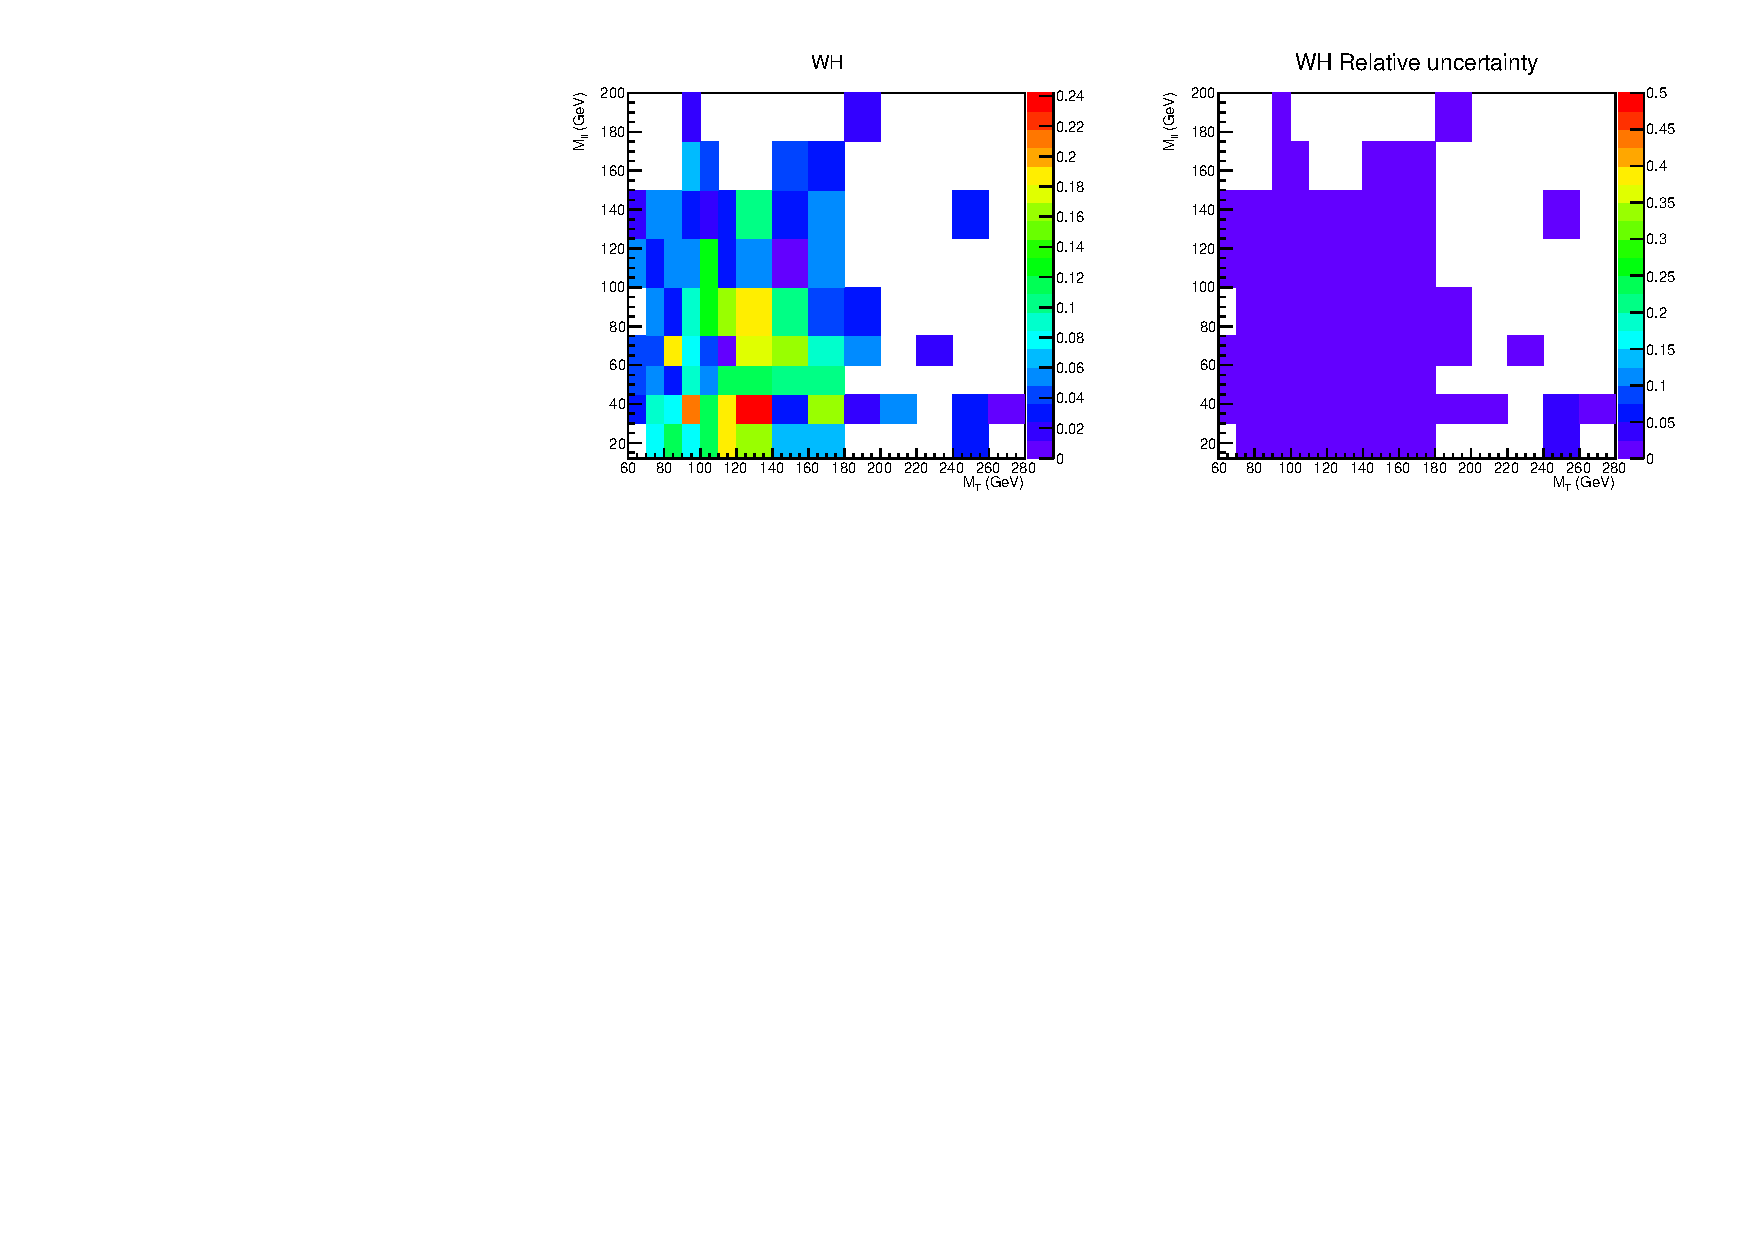
\includegraphics[width=0.8\textwidth]{figures/2dtemplate_WH_mH125_0j.pdf}
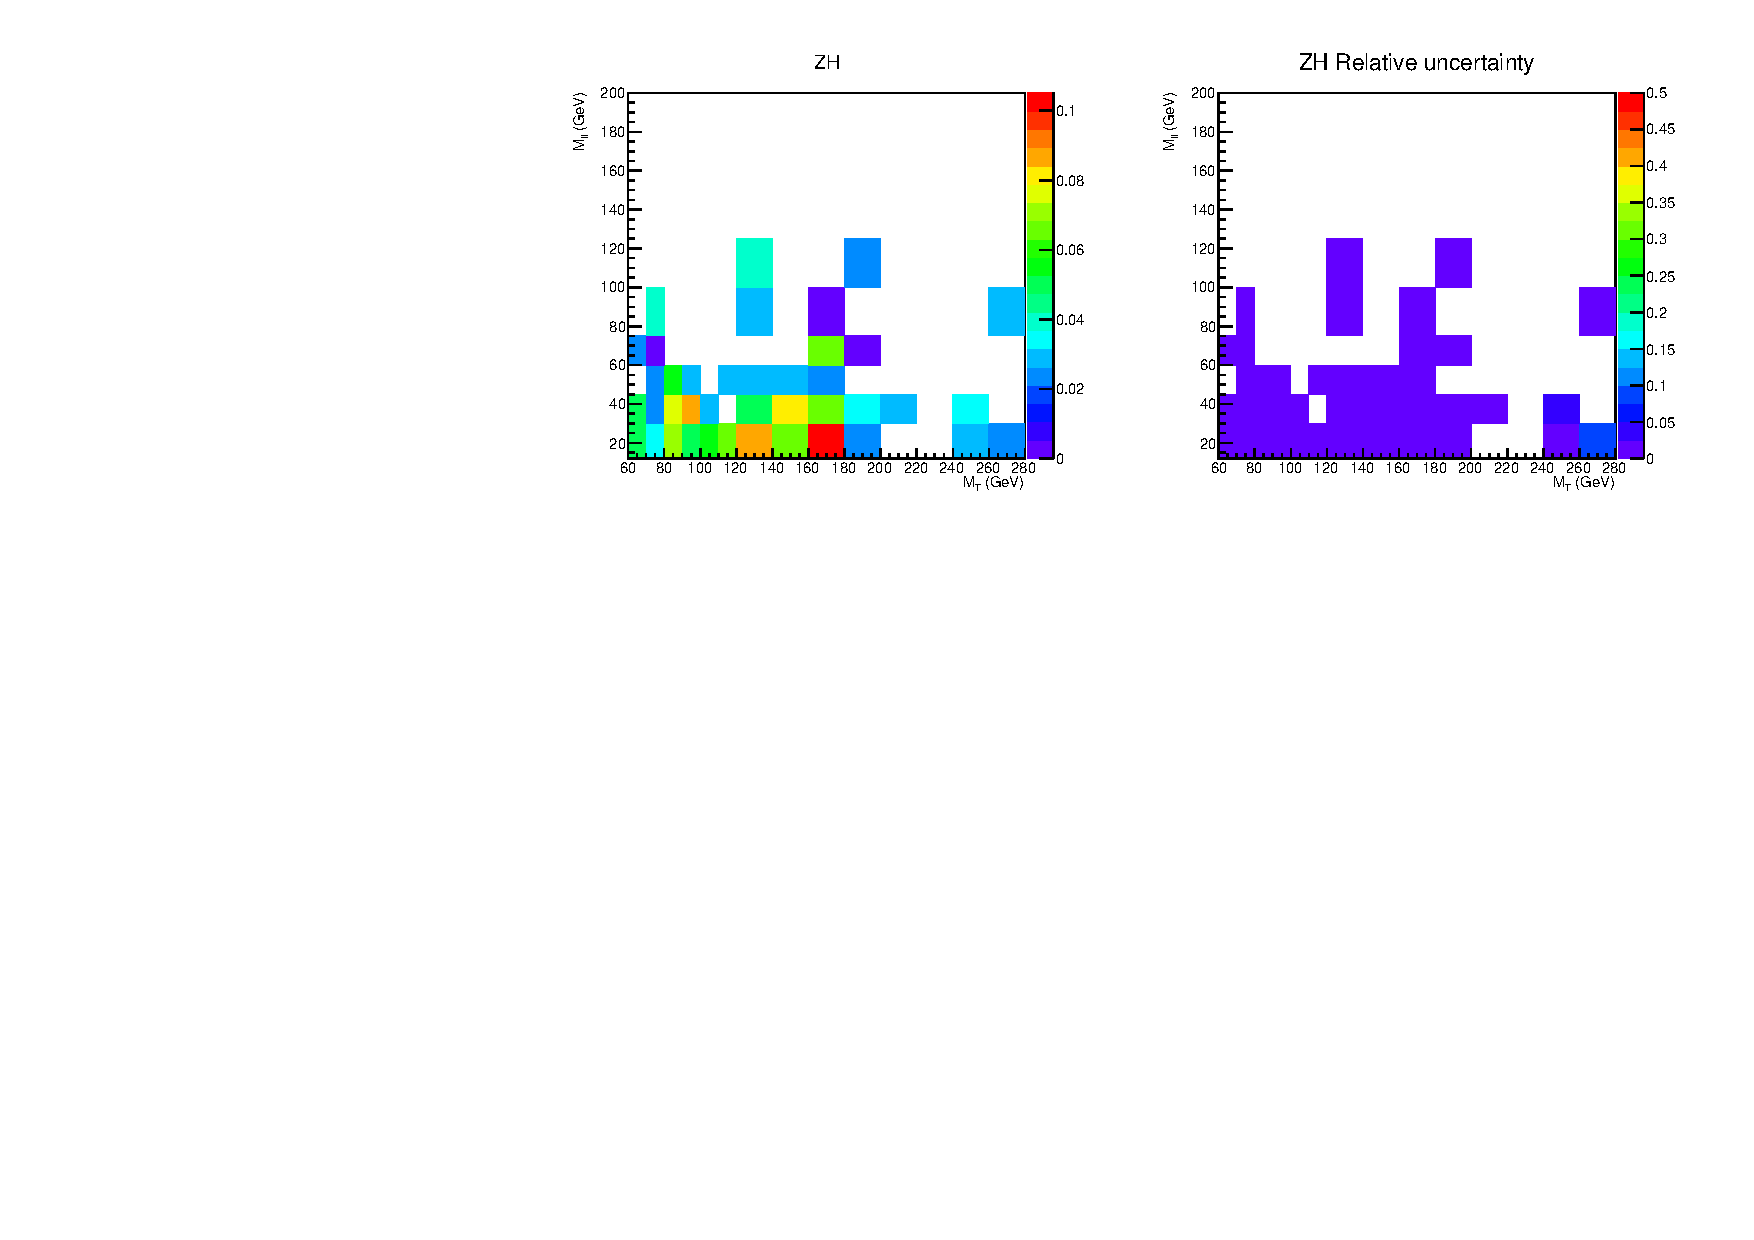
\includegraphics[width=0.8\textwidth]{figures/2dtemplate_ZH_mH125_0j.pdf}
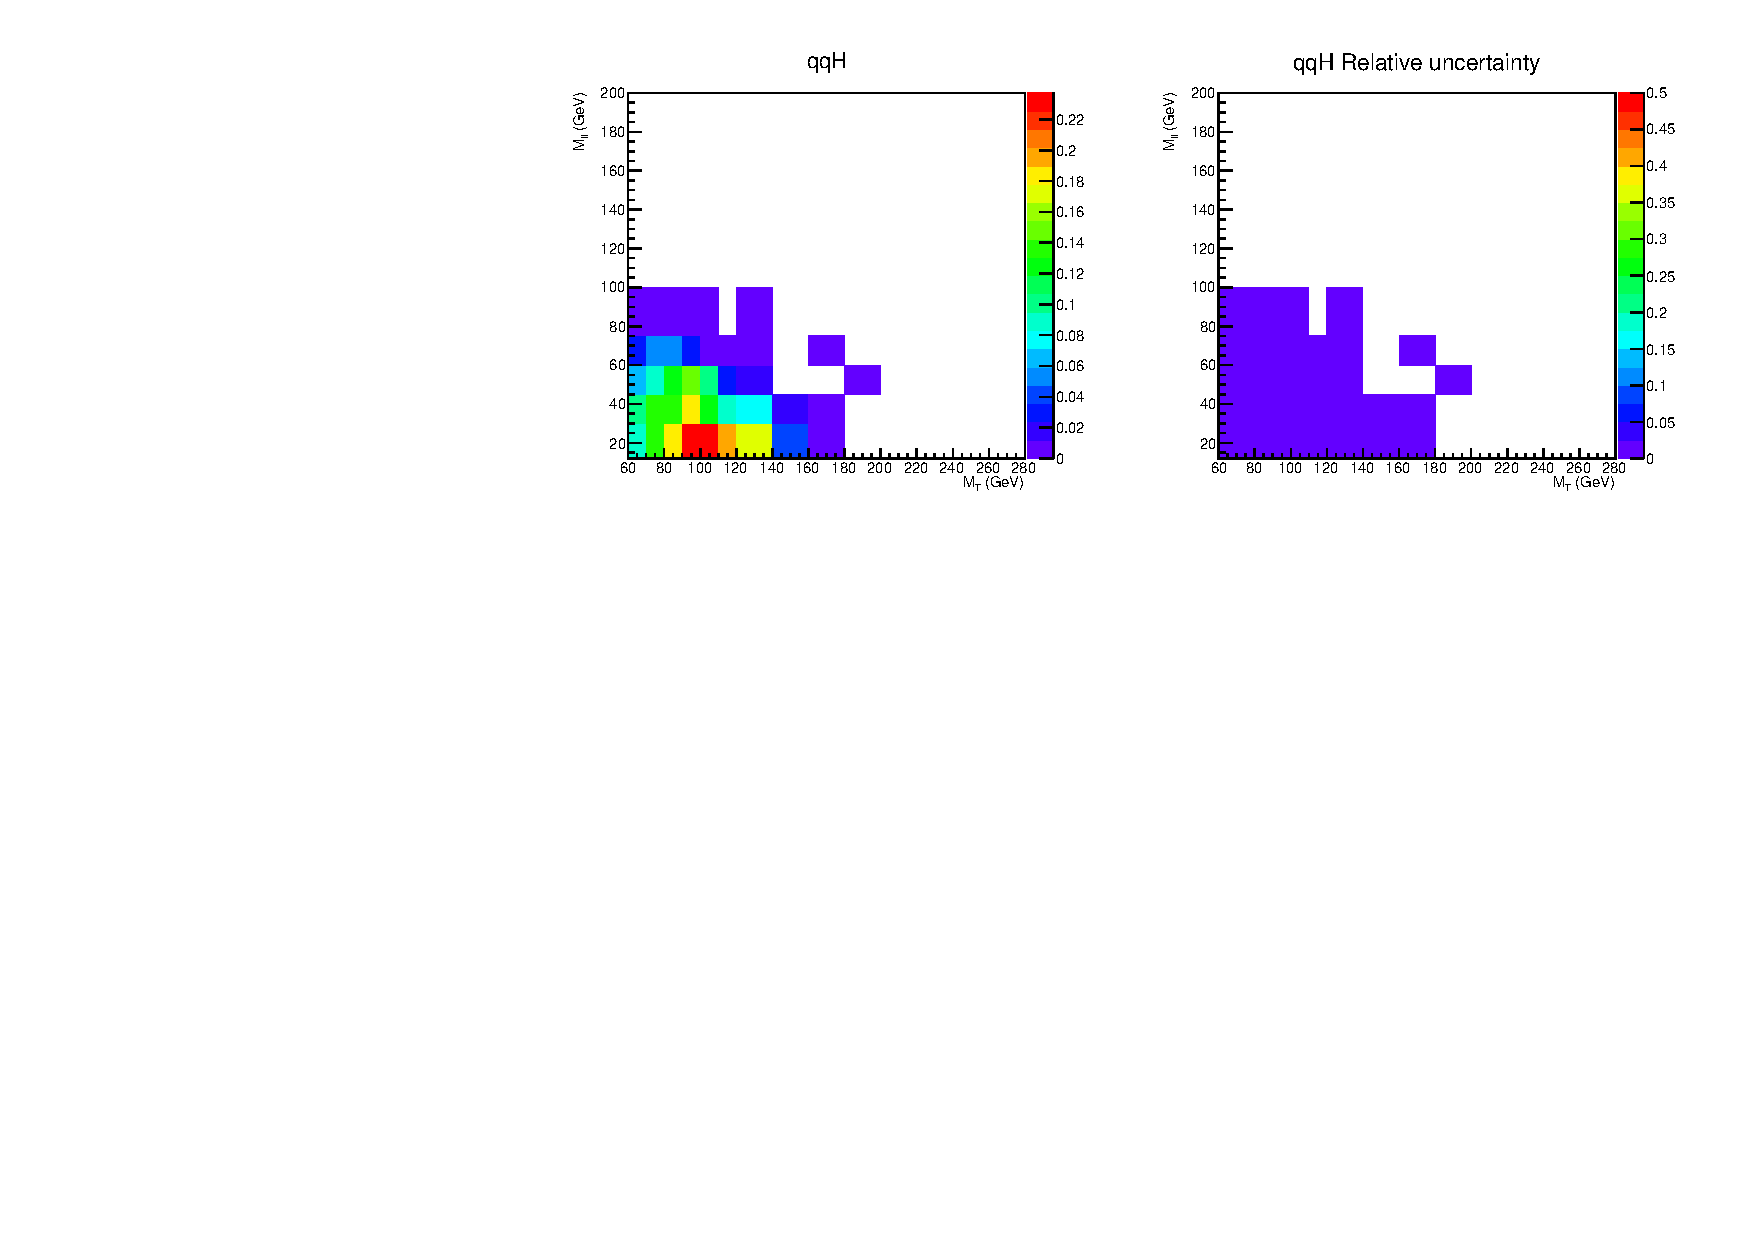
\includegraphics[width=0.8\textwidth]{figures/2dtemplate_qqH_mH125_0j.pdf}
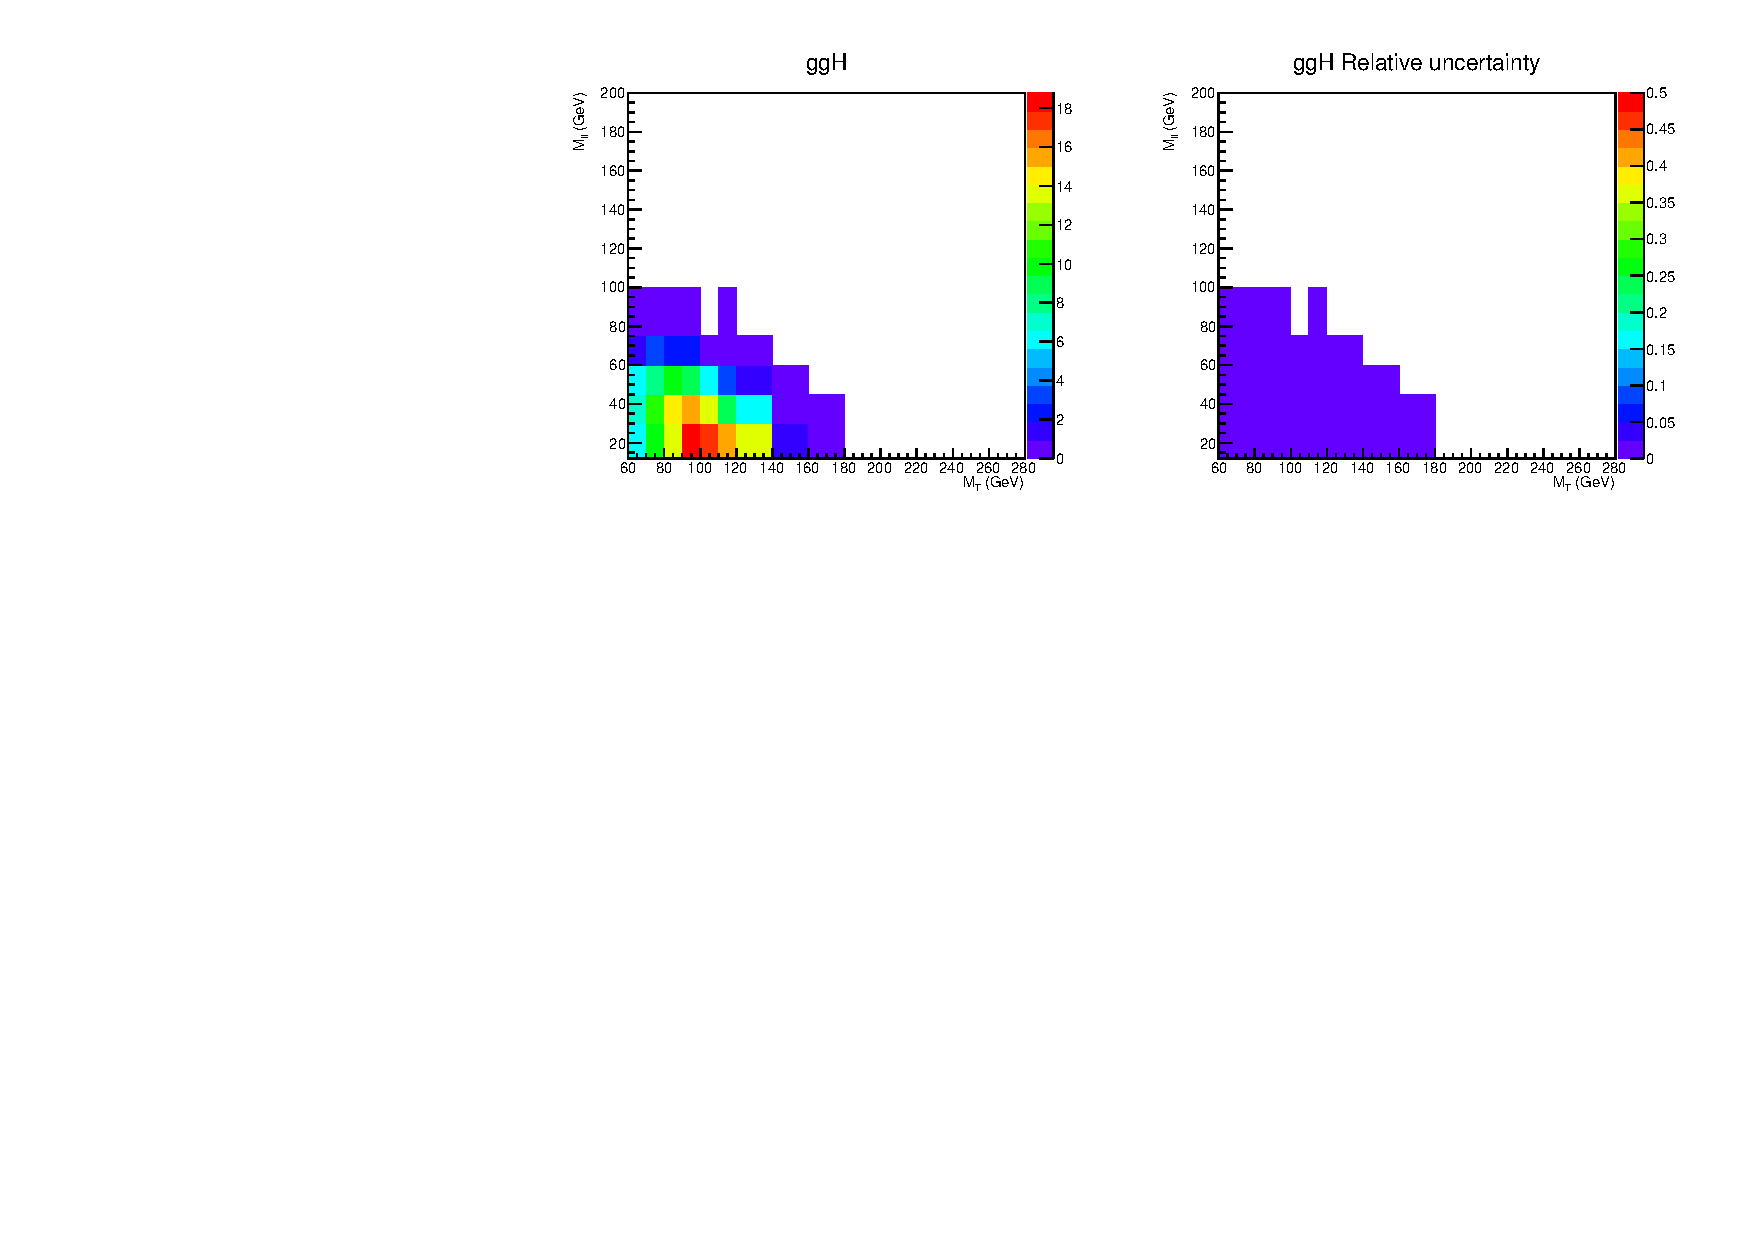
\includegraphics[width=0.8\textwidth]{figures/2dtemplate_ggH_mH125_0j.pdf}
\caption{Templates on the left and relative statistical uncertainty of the MC sample 
on the right of \qqWH, \qqZH, \qqH\ and \ggH. 
The templates are for \mHi\ = 125 \GeV\ analysis in the 0-jet category.
}
\label{fig:2dtemplate_125_0j_1}
\end{figure}

\begin{figure}[htp]
\centering
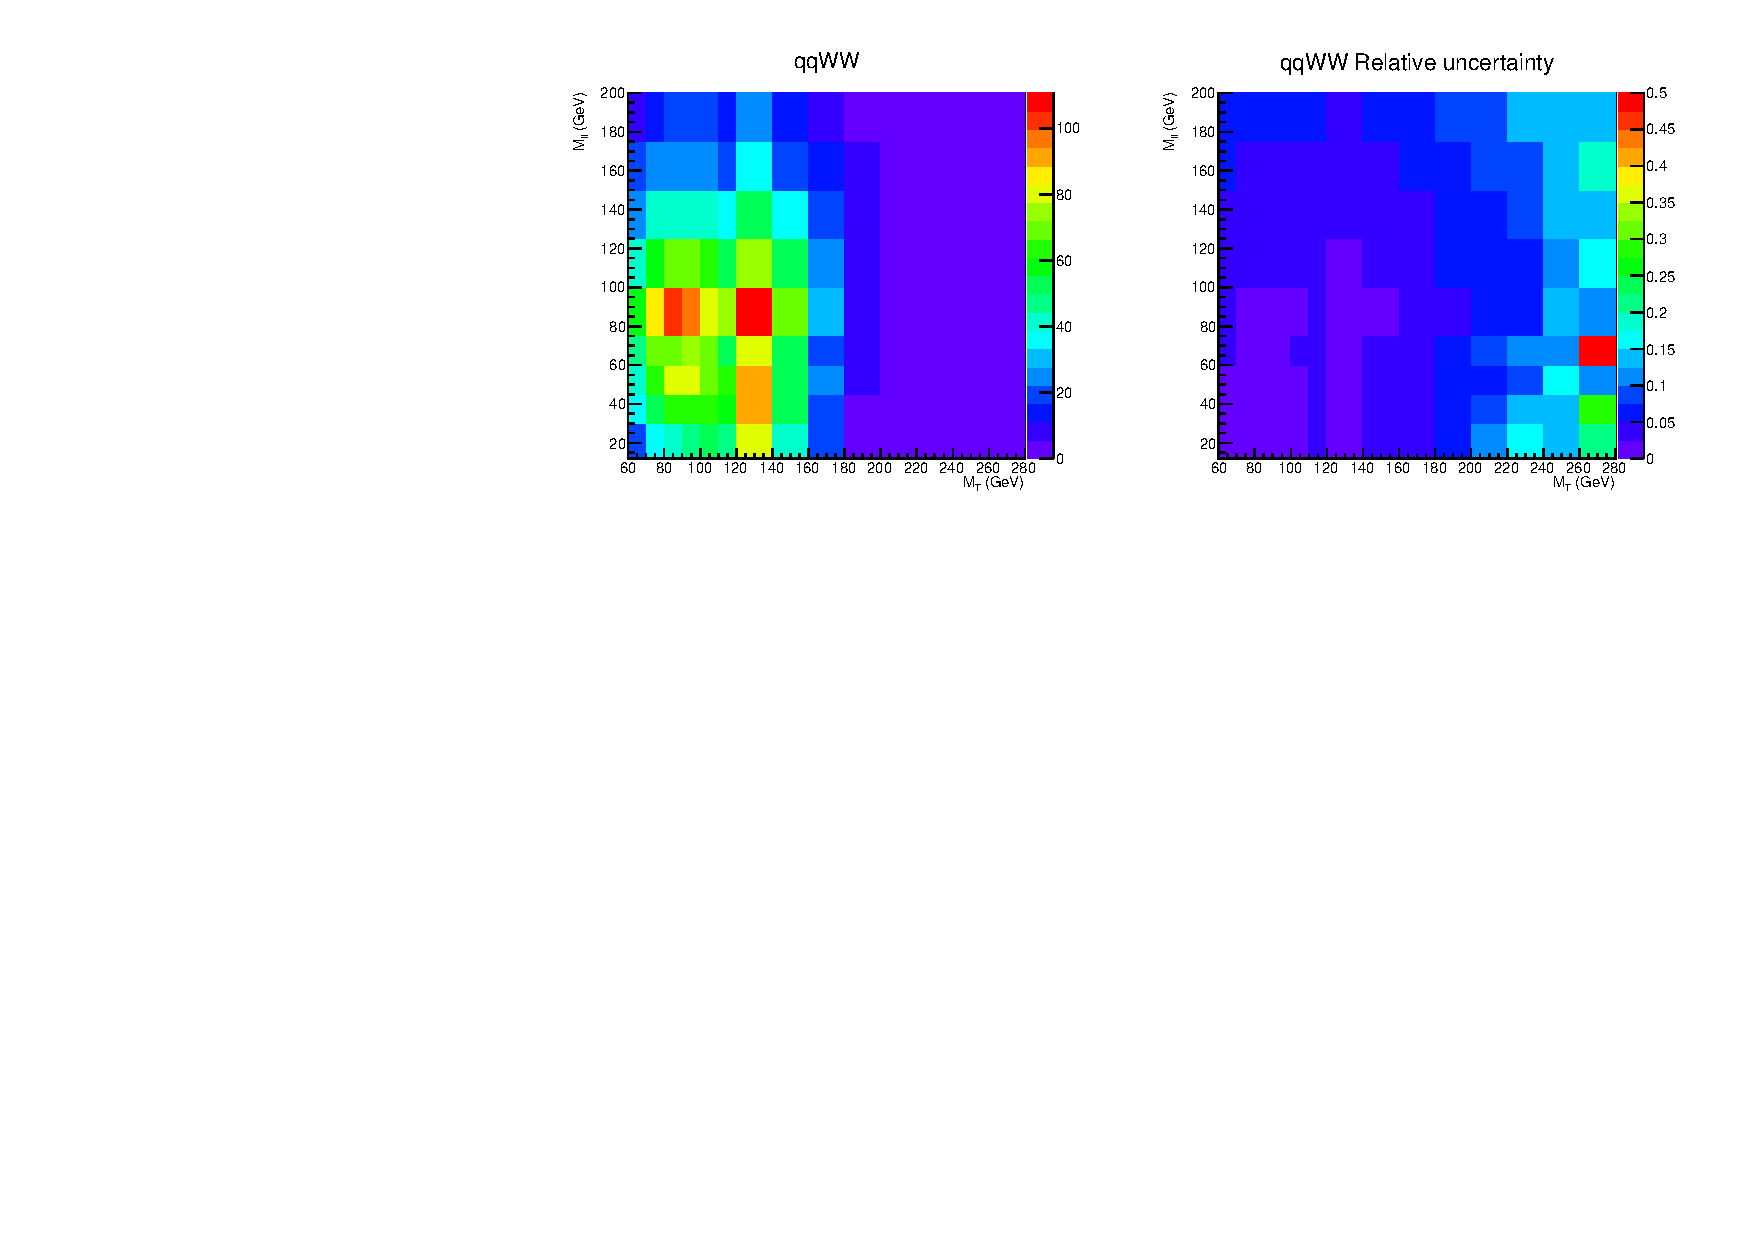
\includegraphics[width=0.8\textwidth]{figures/2dtemplate_qqWW_mH125_0j.pdf}
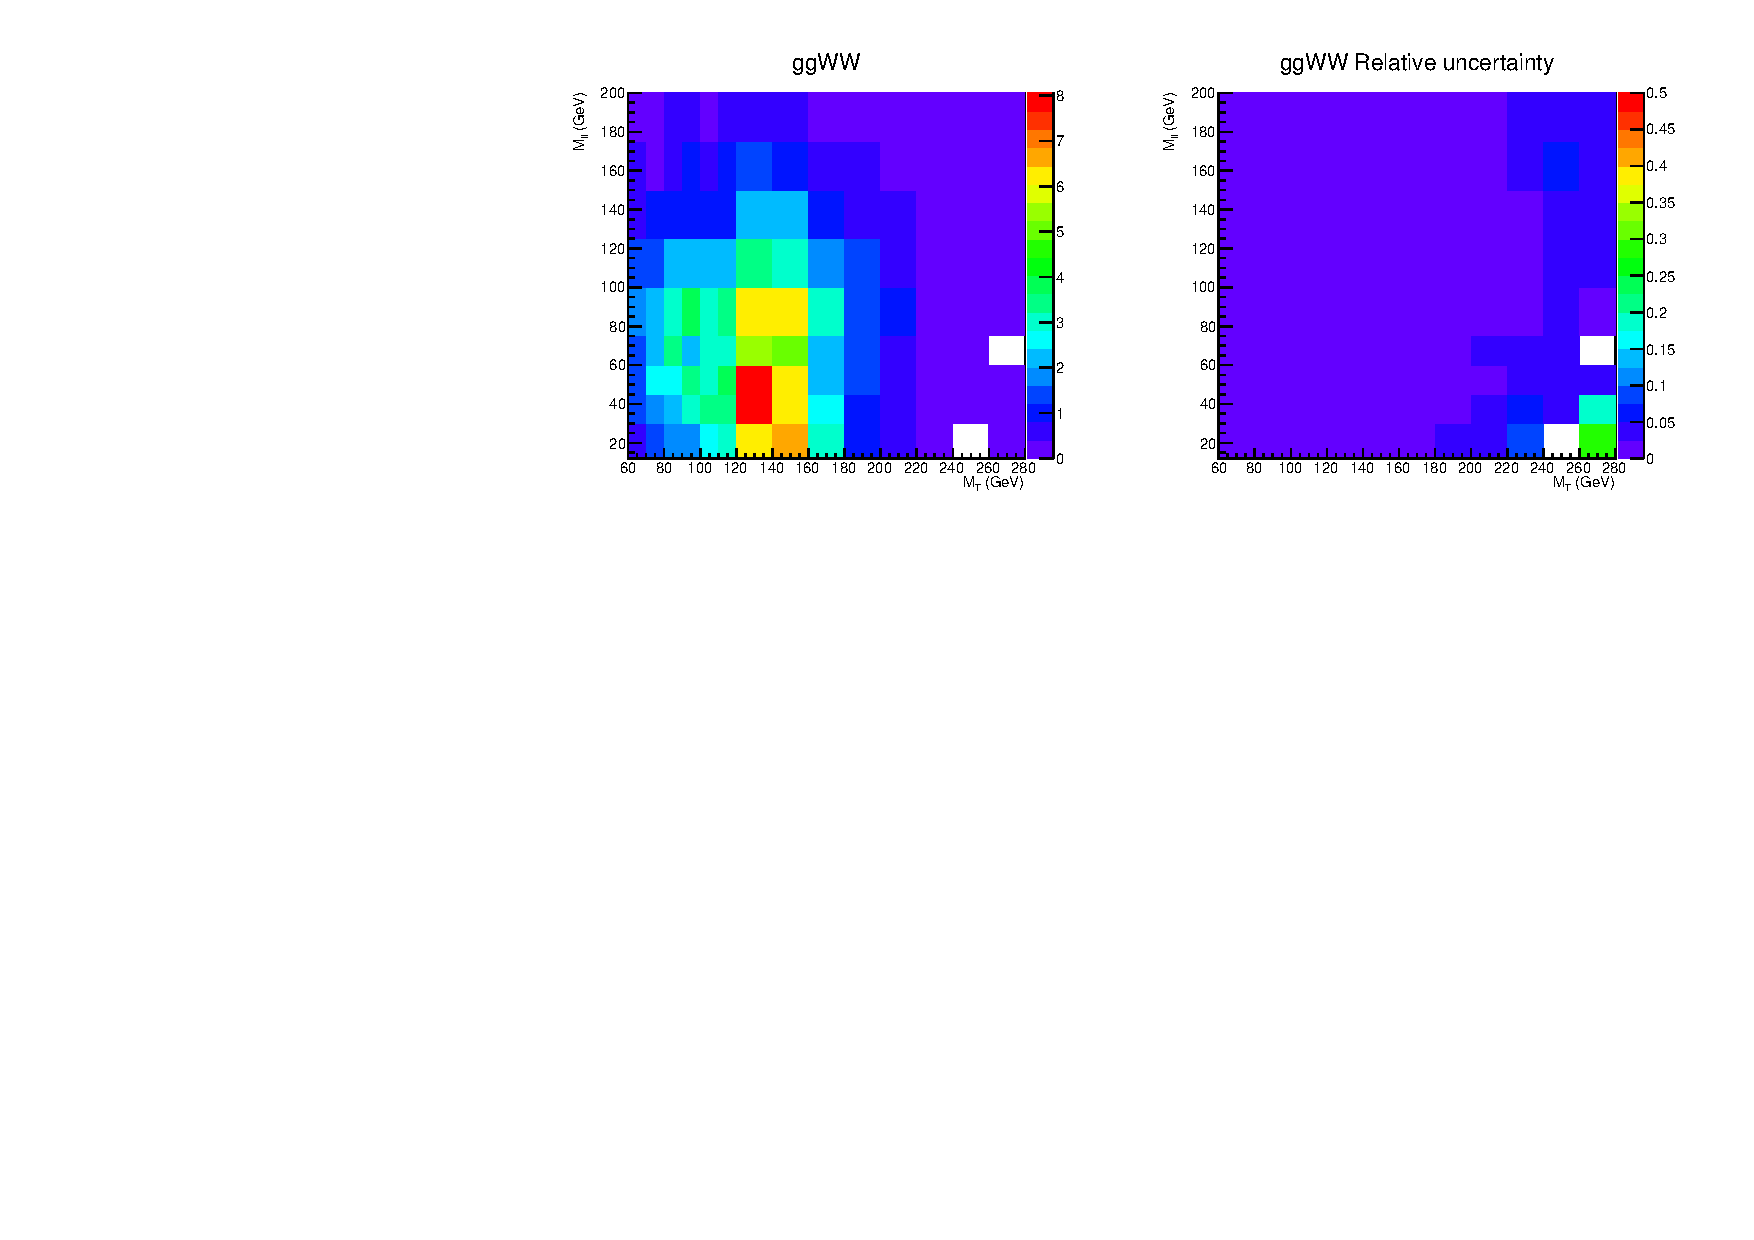
\includegraphics[width=0.8\textwidth]{figures/2dtemplate_ggWW_mH125_0j.pdf}
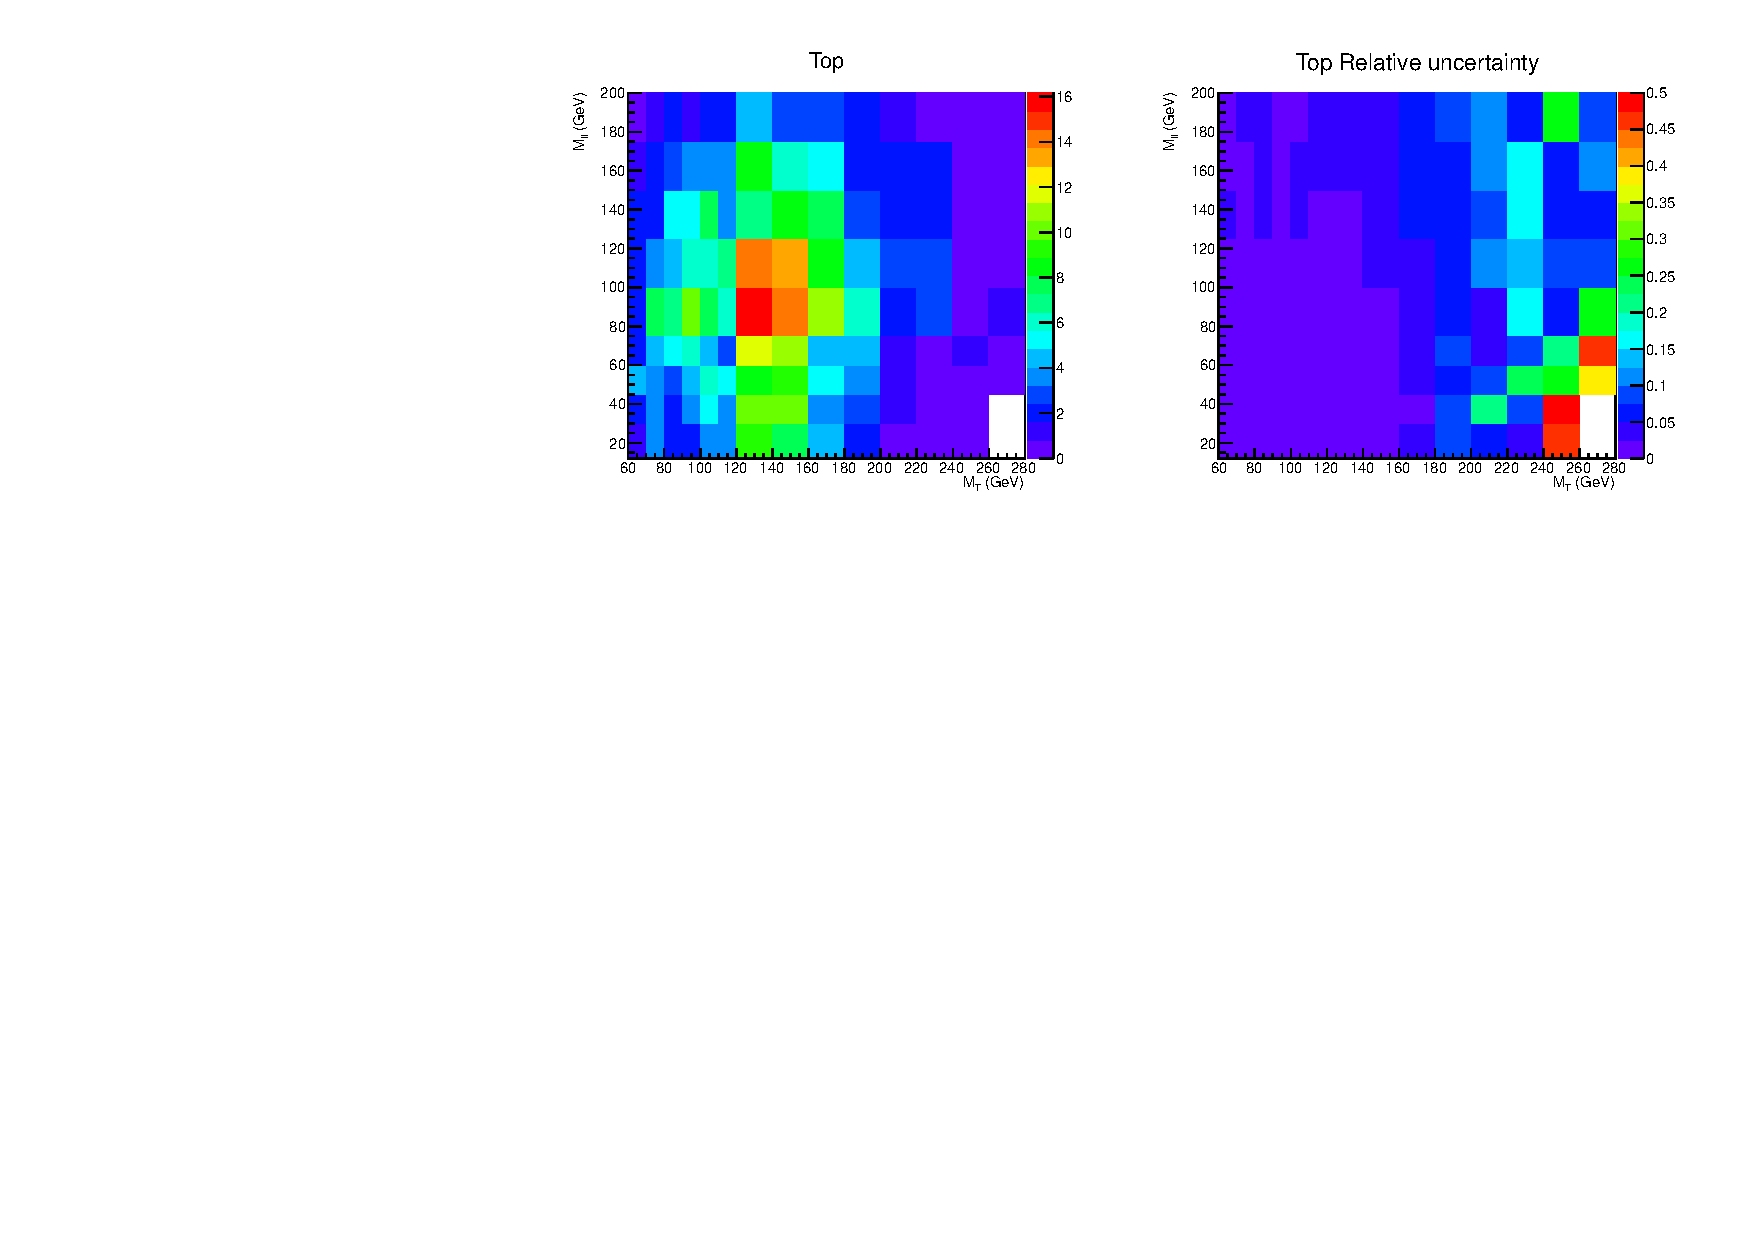
\includegraphics[width=0.8\textwidth]{figures/2dtemplate_Top_mH125_0j.pdf}
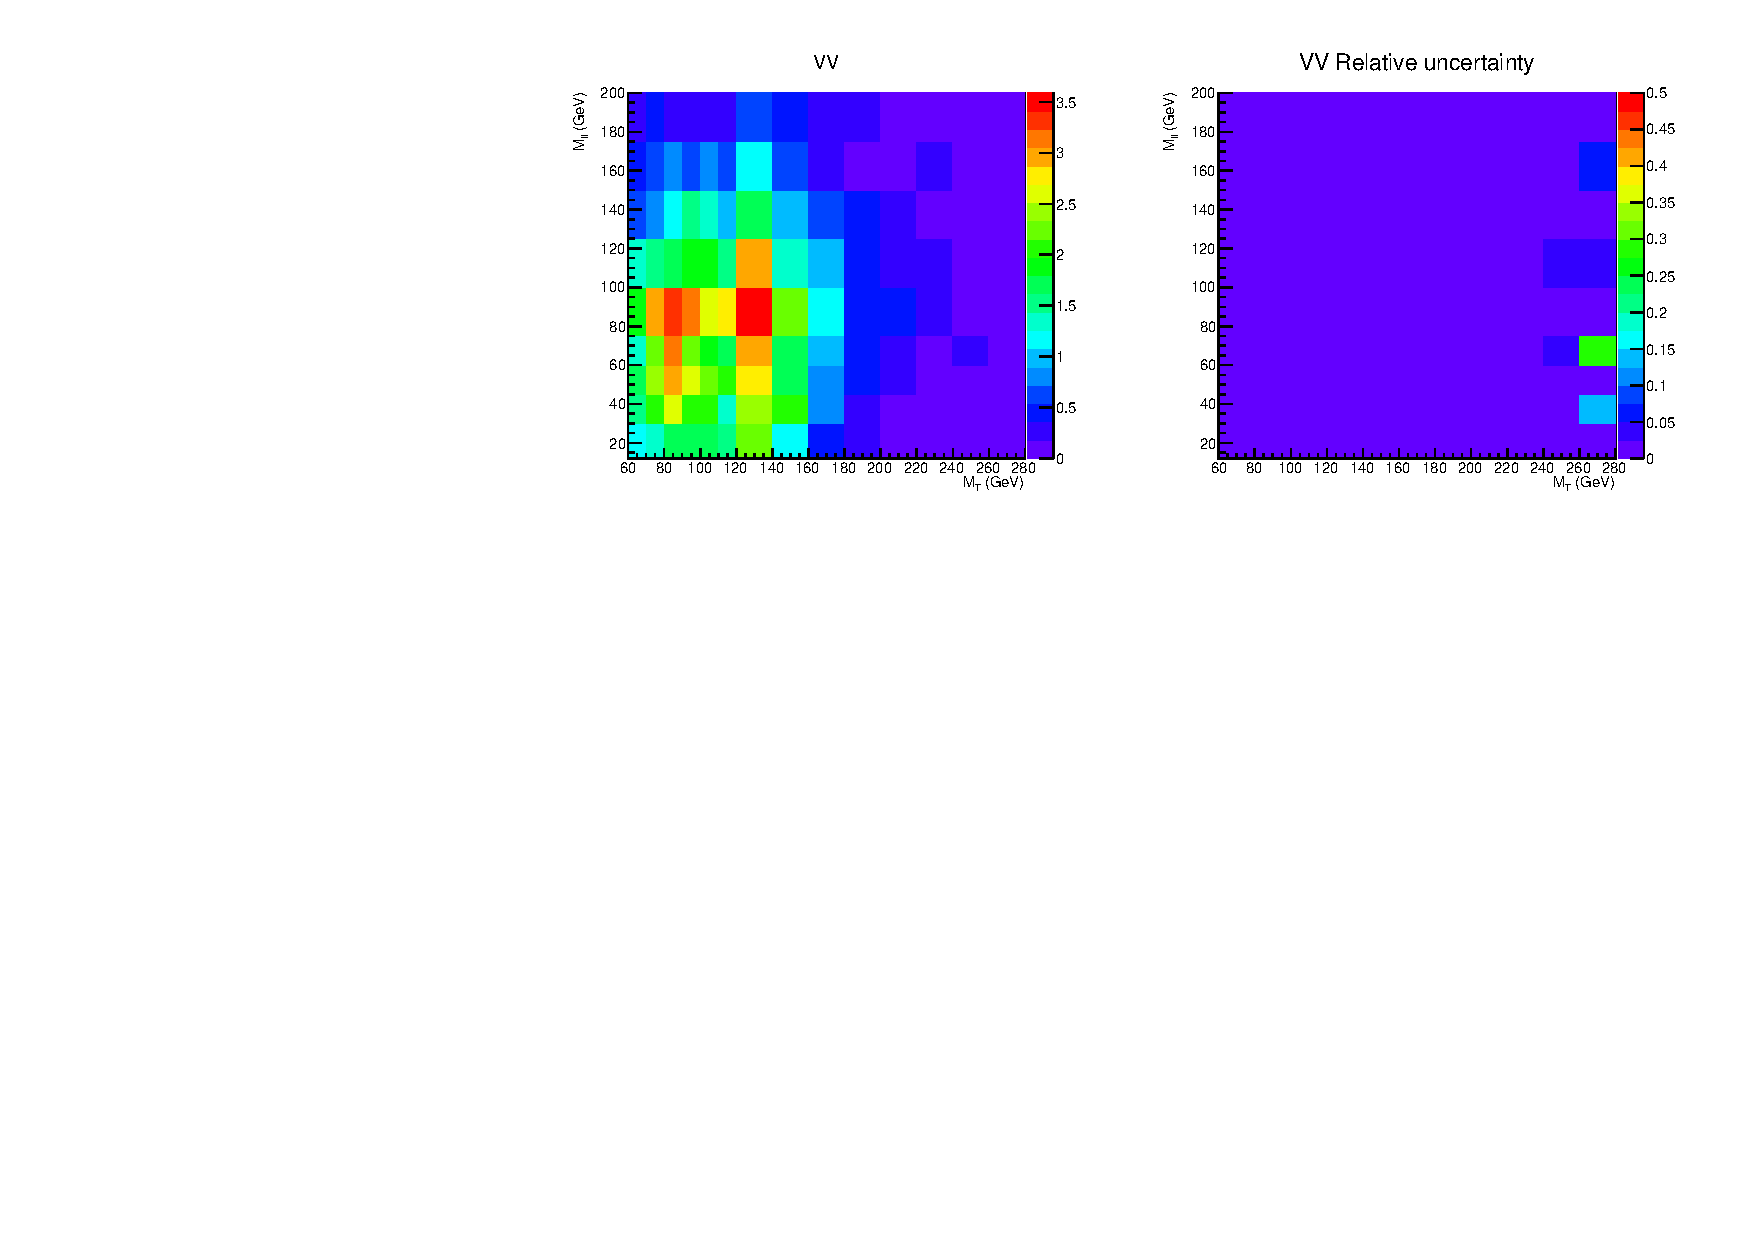
\includegraphics[width=0.8\textwidth]{figures/2dtemplate_VV_mH125_0j.pdf}
\caption{Templates on the left and relative statistical uncertainty of the MC sample
on the right of \qqww, \ggww, \topbkg\ and \vv. 
The templates are for \mHi\ = 125 \GeV\ analysis in the 0-jet category.}
\label{fig:2dtemplate_125_0j_2}
\end{figure}

\begin{figure}[htp]
\centering
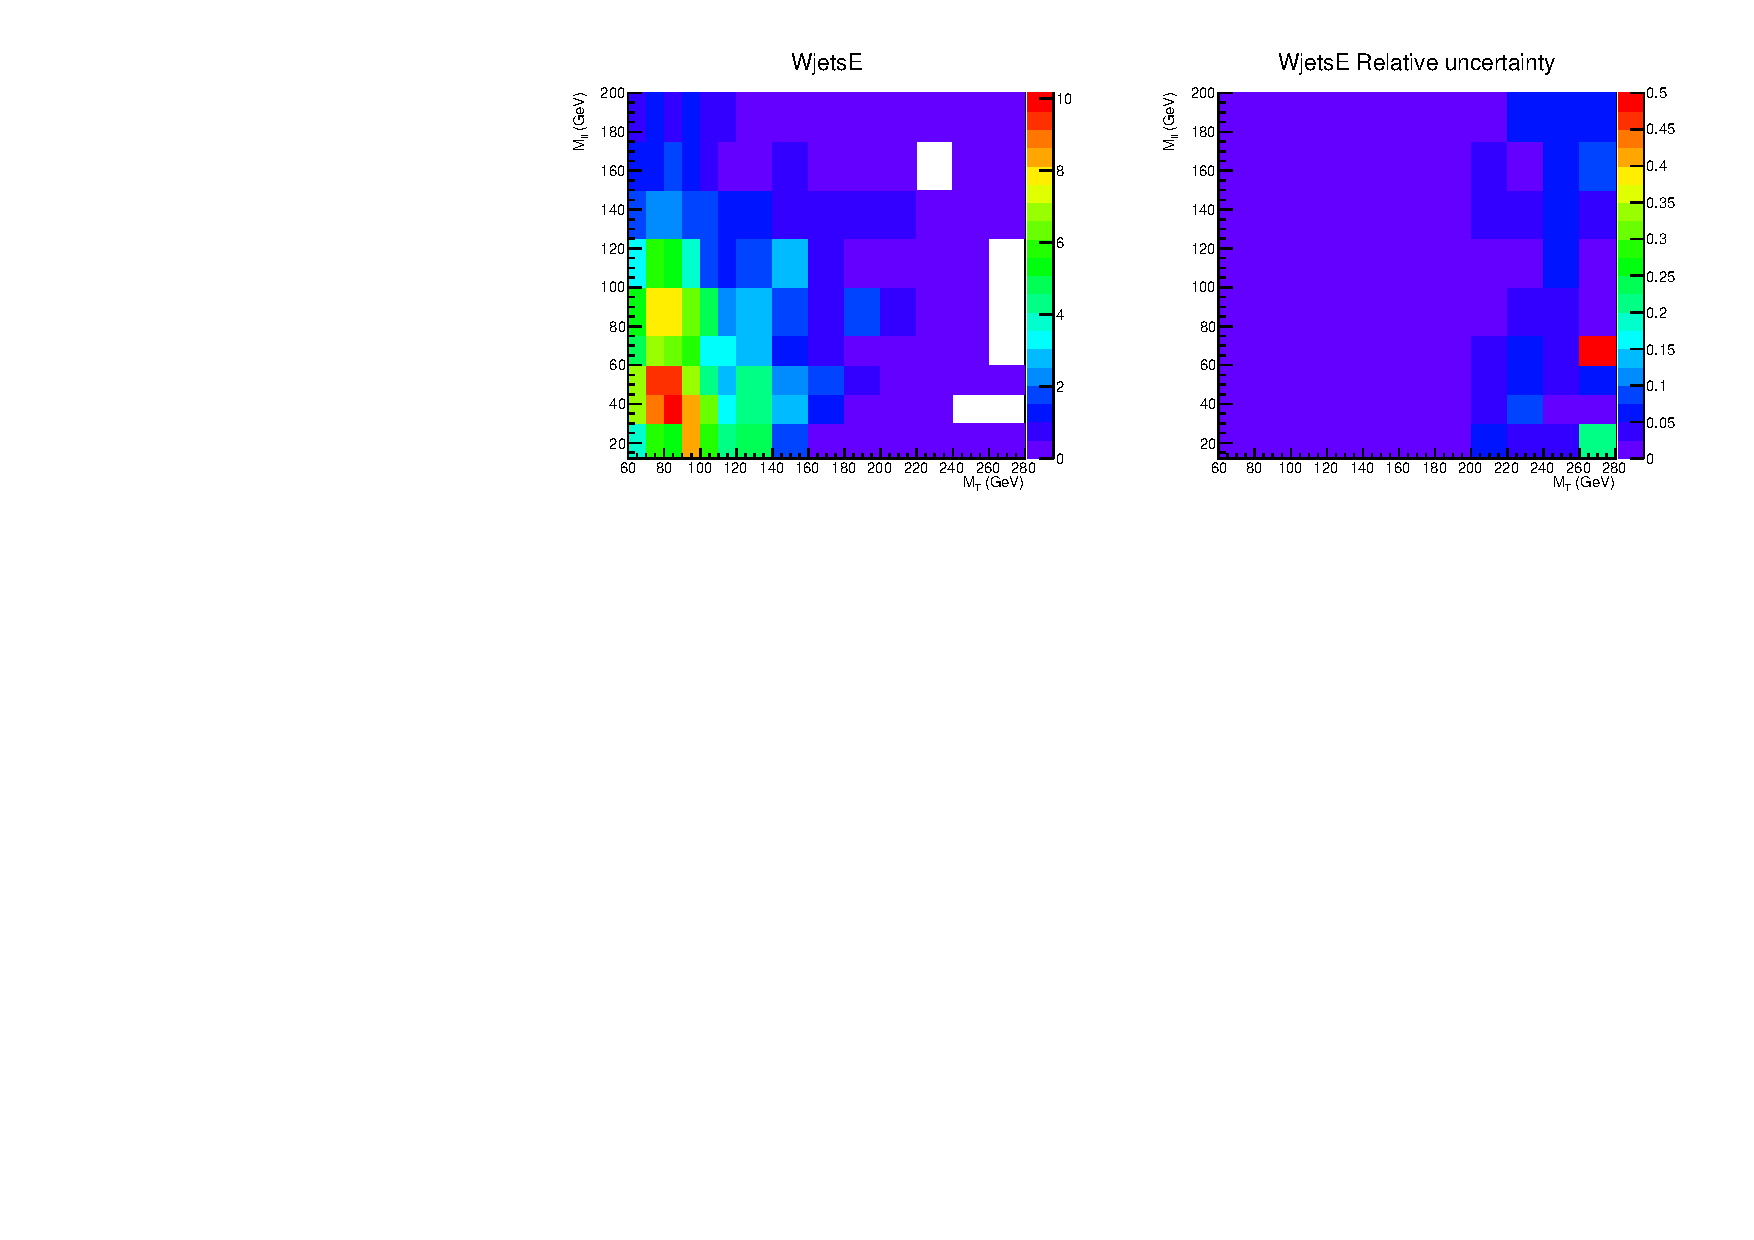
\includegraphics[width=0.8\textwidth]{figures/2dtemplate_WjetsE_mH125_0j.pdf}
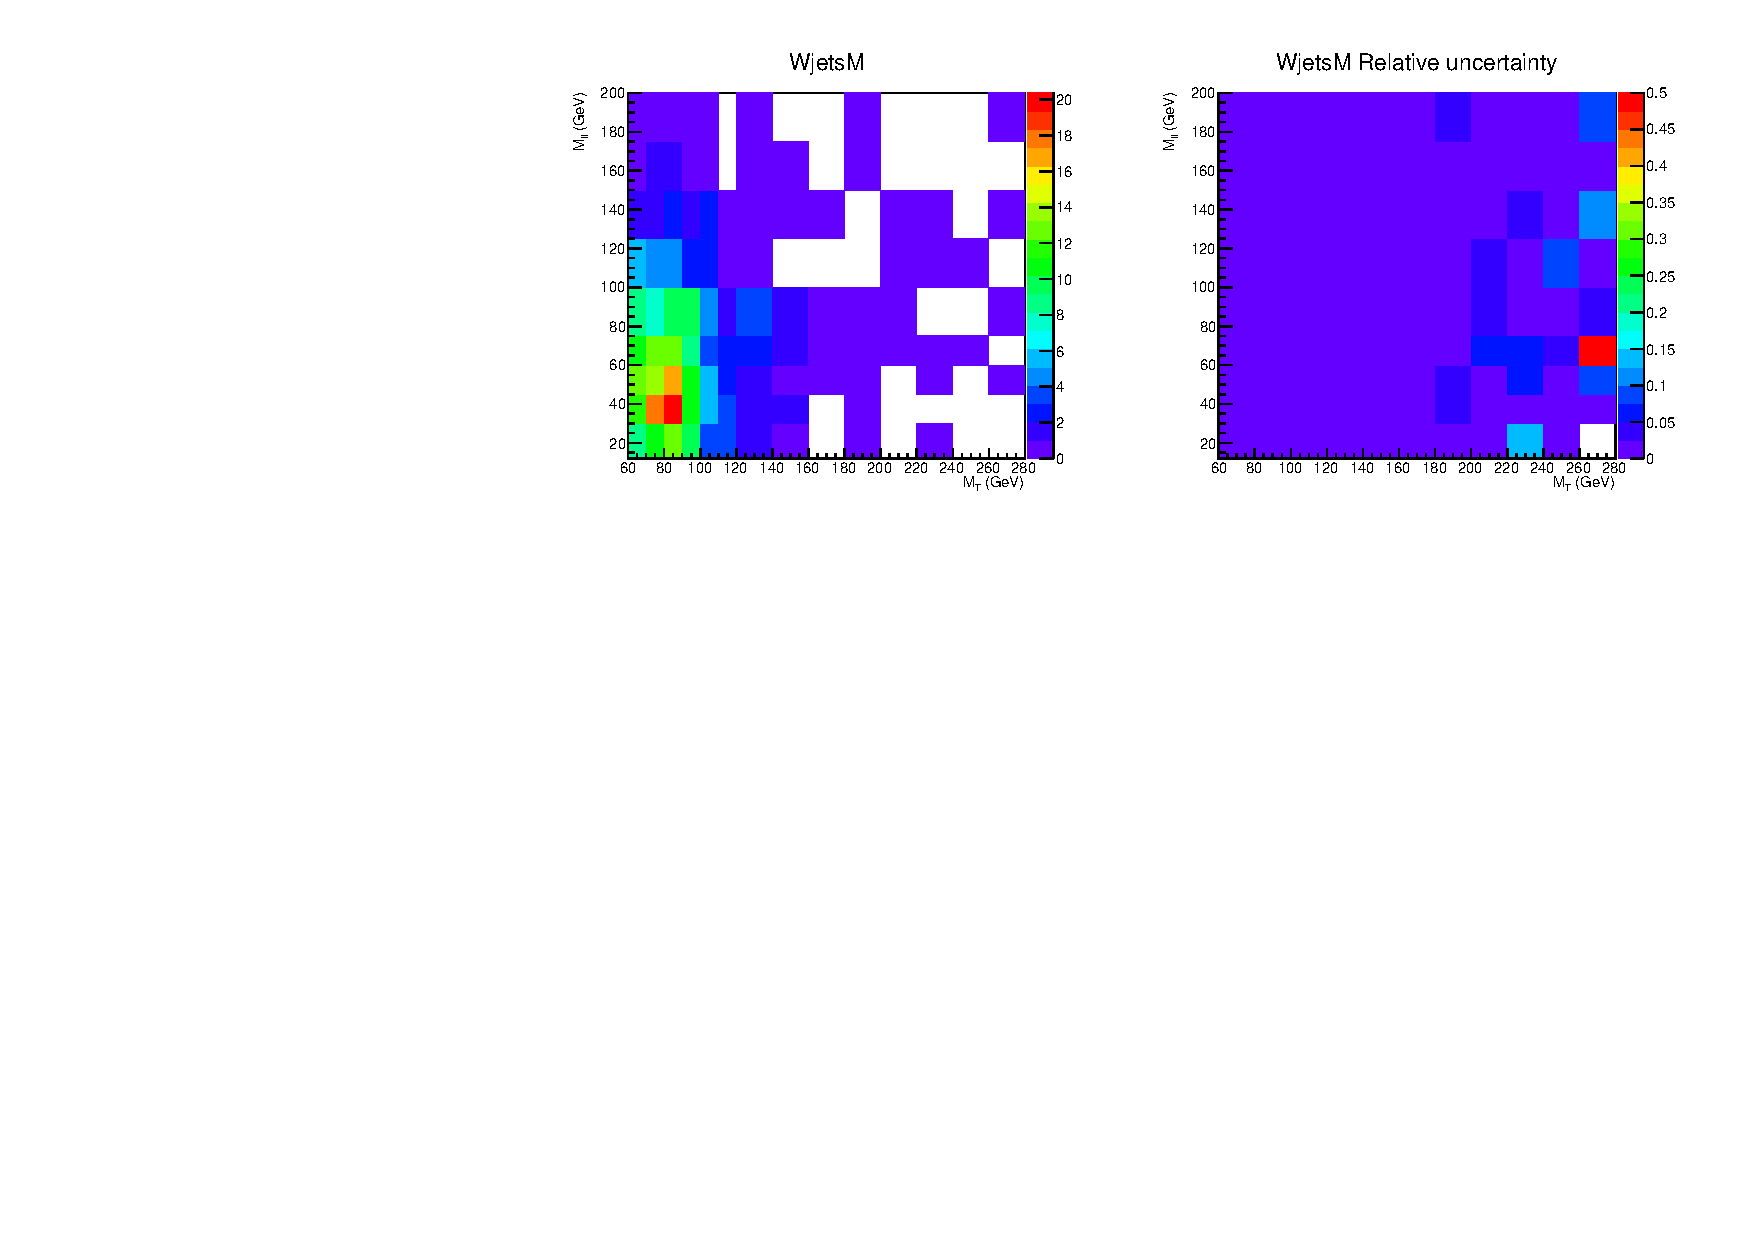
\includegraphics[width=0.8\textwidth]{figures/2dtemplate_WjetsM_mH125_0j.pdf}
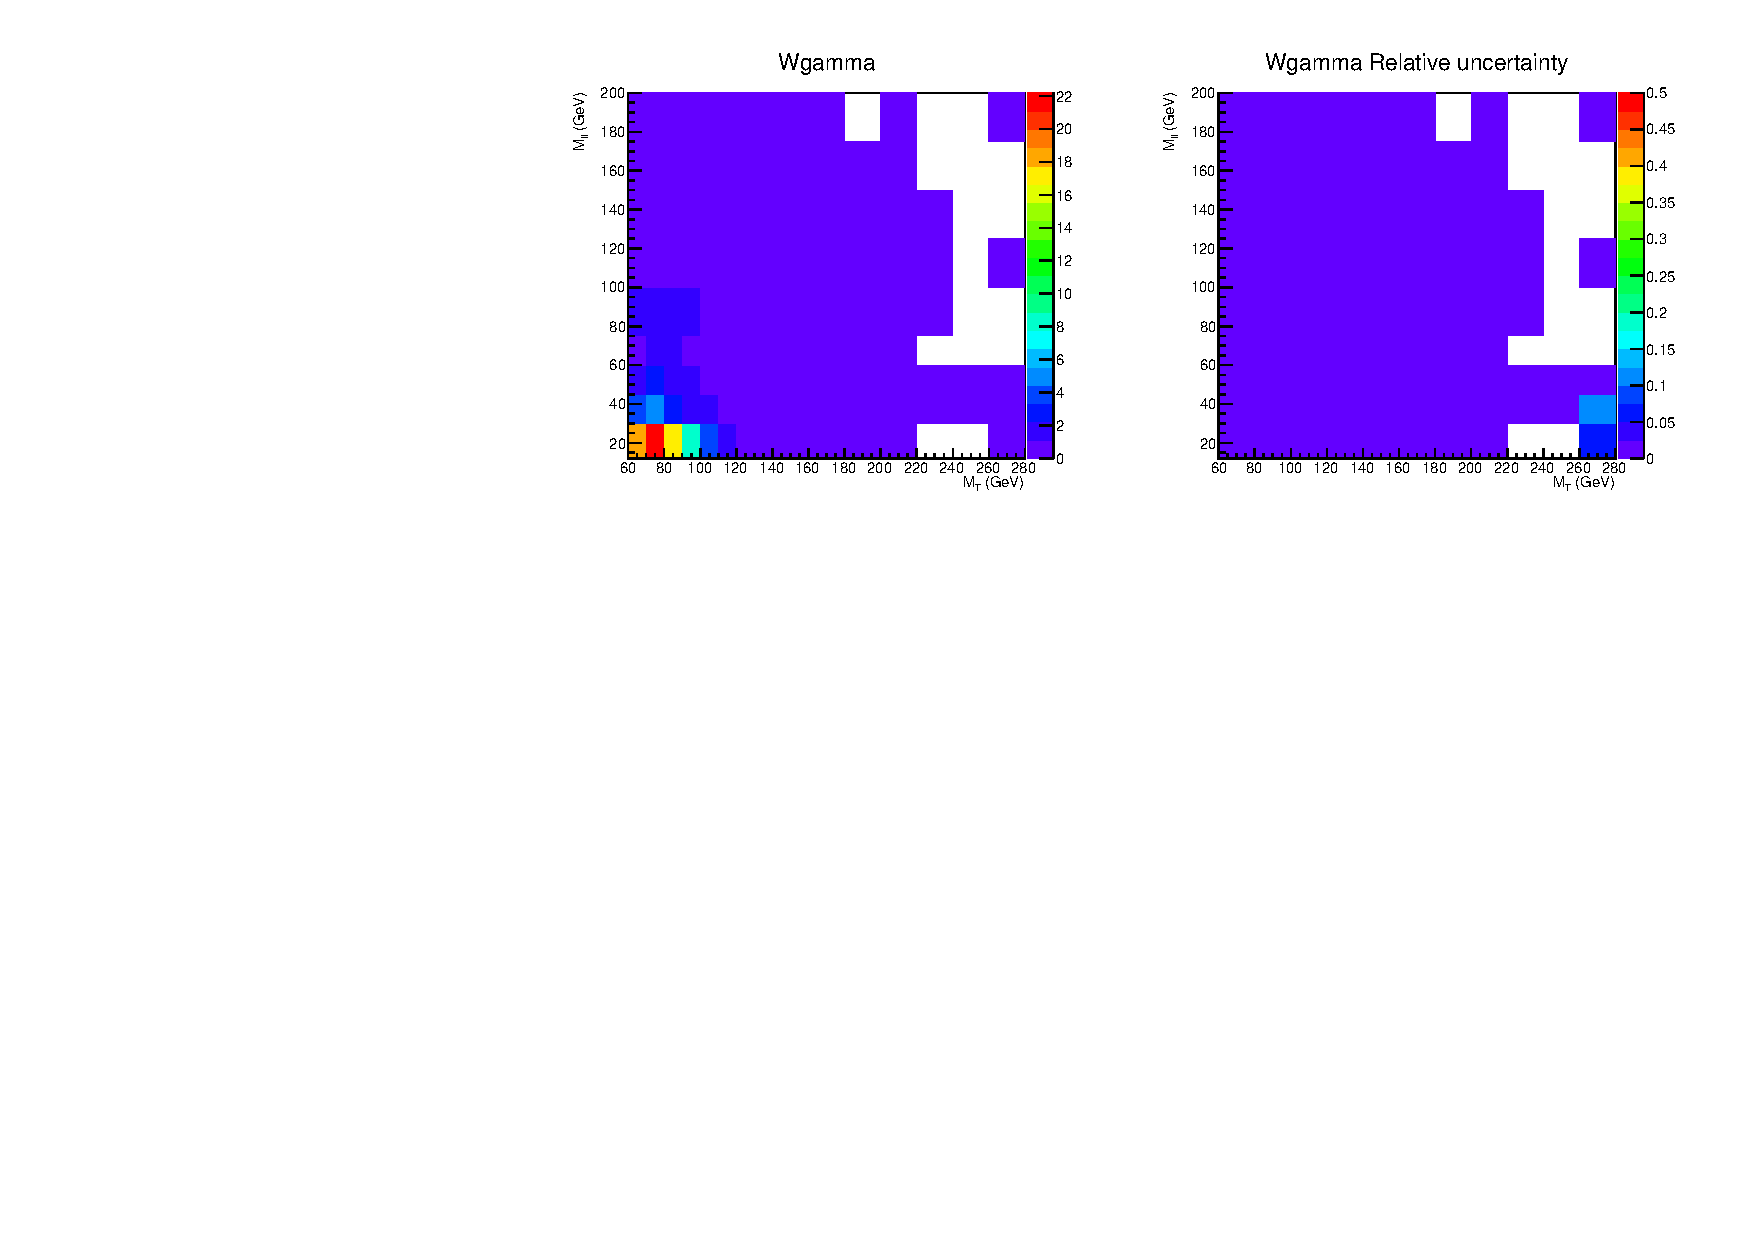
\includegraphics[width=0.8\textwidth]{figures/2dtemplate_Wgamma_mH125_0j.pdf}
\caption{Templates on the left and relative statistical uncertainty of the MC sample
on the right of \WjetsE, \WjetsM\ and \wgamma. 
The templates are for \mHi\ = 125 \GeV\ analysis in the 0-jet category.}
\label{fig:2dtemplate_125_0j_3}
\end{figure}

\begin{figure}[htp]
\centering
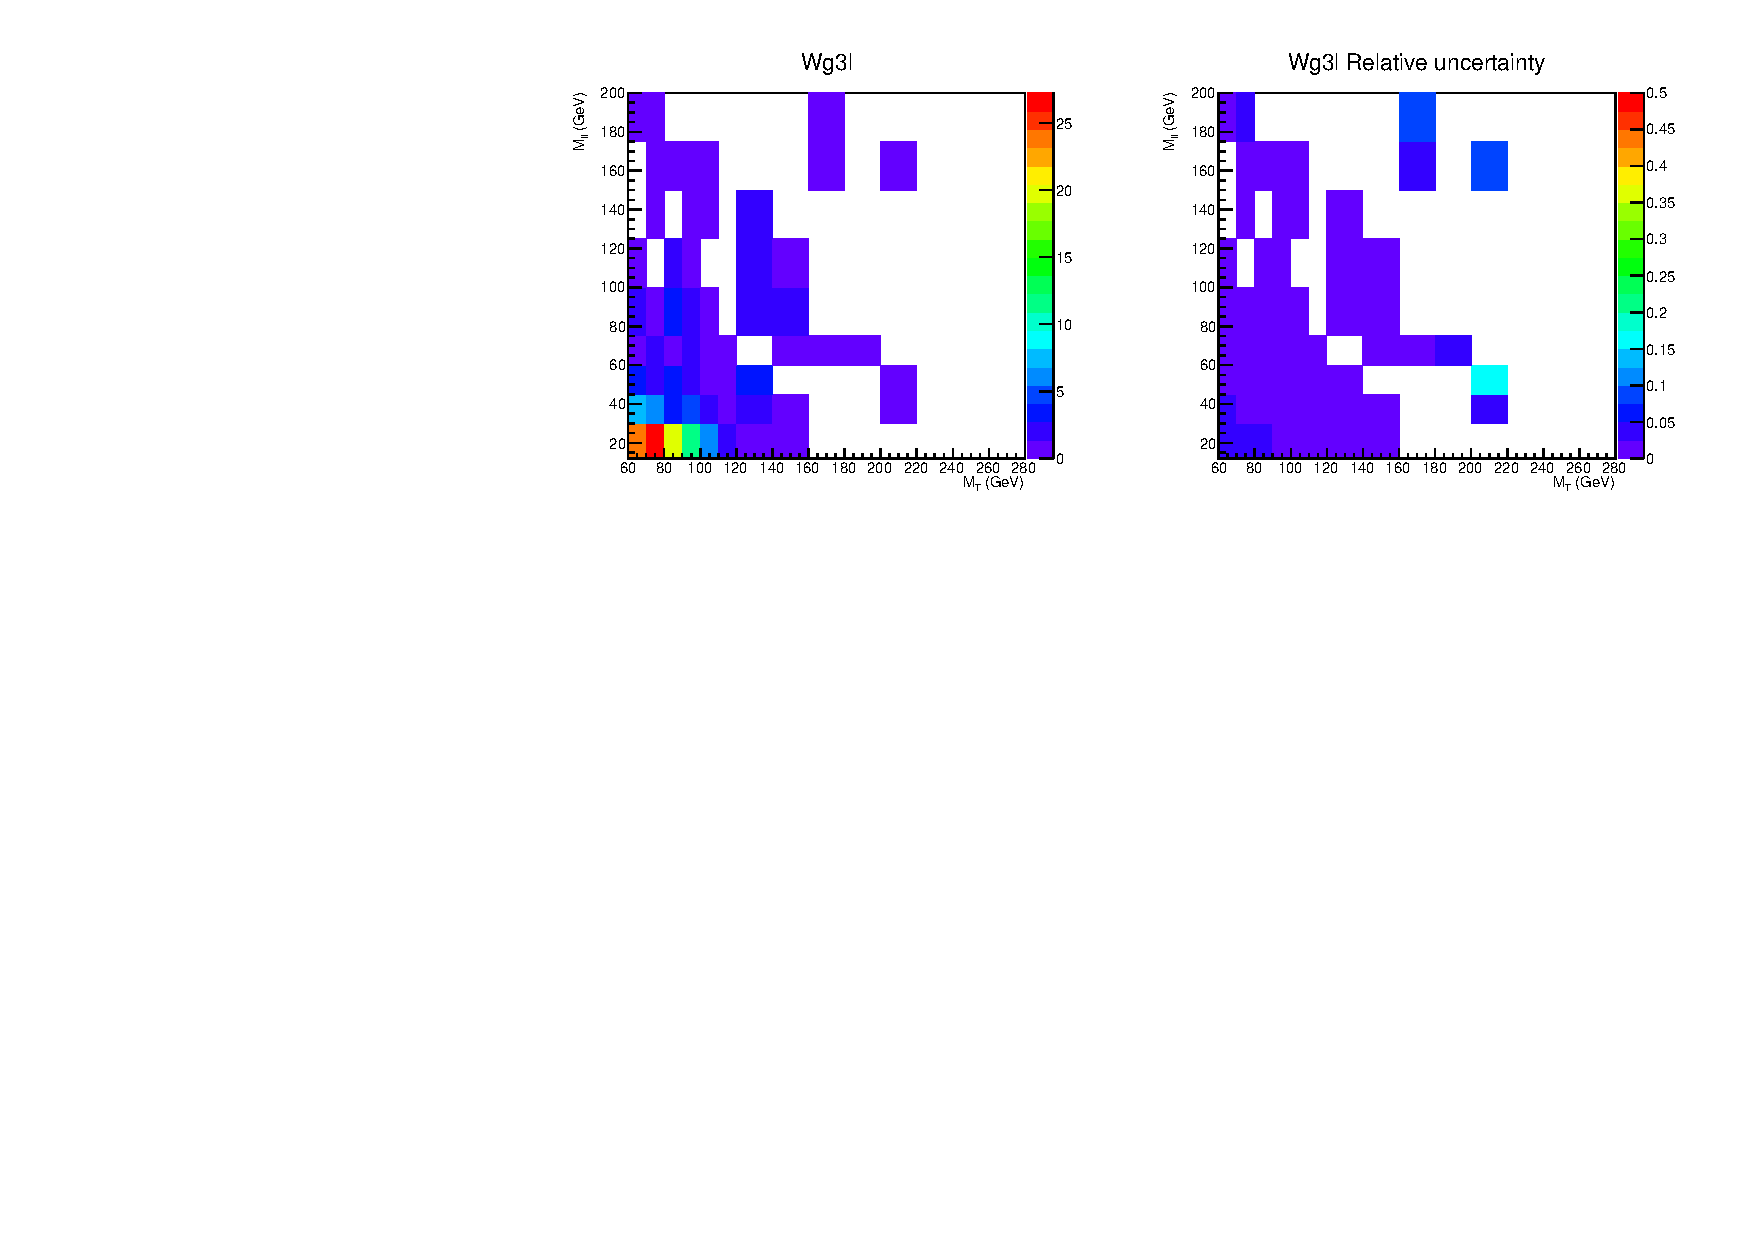
\includegraphics[width=0.8\textwidth]{figures/2dtemplate_Wg3l_mH125_0j.pdf}
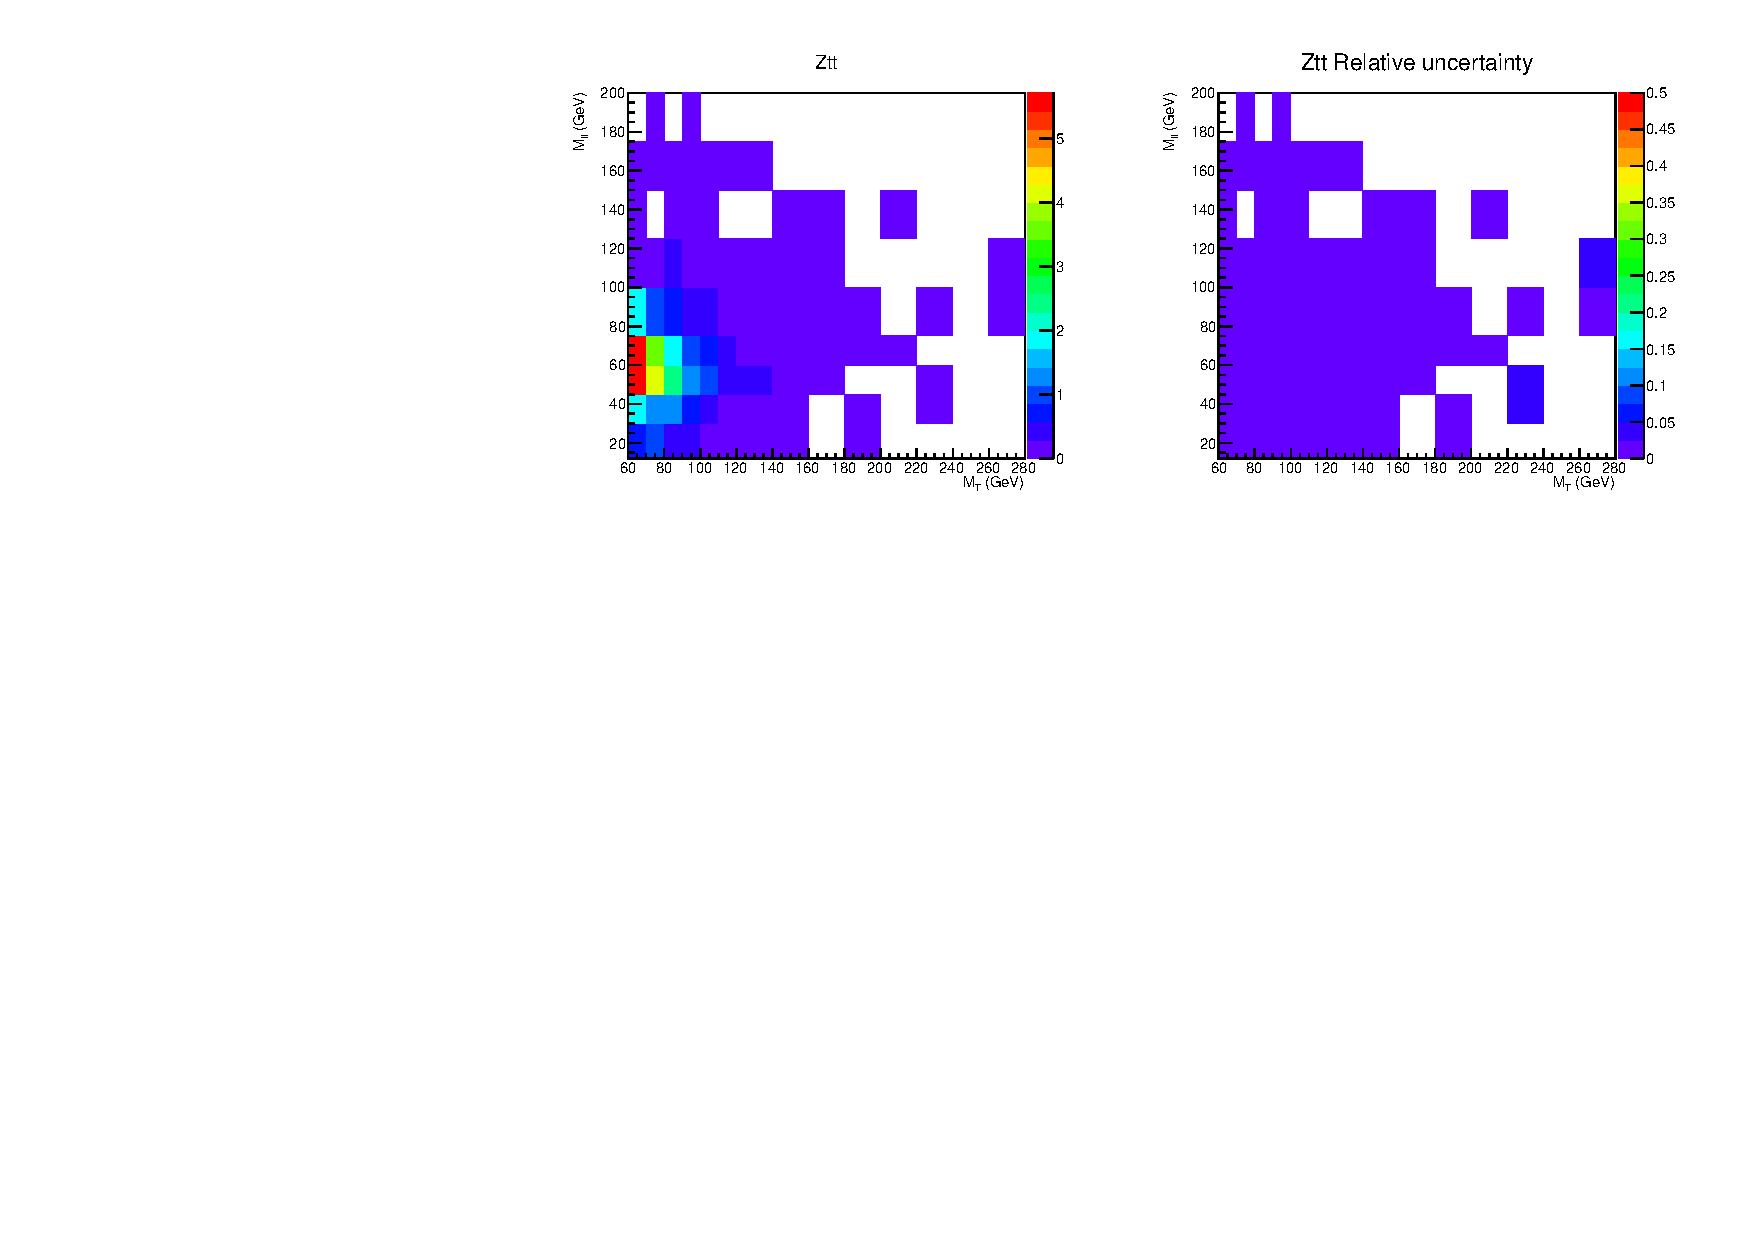
\includegraphics[width=0.8\textwidth]{figures/2dtemplate_Ztt_mH125_0j.pdf}
\caption{Templates on the left and relative statistical uncertainty of the MC sample
on the right of \wgammastar\ and \ztt. 
The templates are for \mHi\ = 125 \GeV\ analysis in the 0-jet category.}
\label{fig:2dtemplate_125_0j_4}
\end{figure}
